\documentclass[a4paper,12pt]{report}
\usepackage[utf8]{inputenc}
\usepackage[german]{babel}
\usepackage{amsmath}
\usepackage{amssymb}
\usepackage{amsthm}
\usepackage{geometry}
\usepackage{graphicx}
\usepackage[hidelinks]{hyperref}
\usepackage{listings}
\usepackage{xcolor}
\usepackage{enumitem}
\usepackage{booktabs}
\usepackage{array}
\usepackage{multirow}
\usepackage{float}
\usepackage{microtype}

\geometry{margin=2.5cm}

\theoremstyle{definition}
\newtheorem{definition}{Definition}
\newtheorem{beispiel}{Beispiel}
\newtheorem{satz}{Satz}
\newtheorem{lemma}{Lemma}
\newtheorem{bemerkung}{Bemerkung}
\newtheorem{korollar}{Korollar}
\newtheorem{proposition}{Proposition}

\setlist[itemize,1]{label=--}

% ---------- Farben ----------
\definecolor{mainblue}{RGB}{25, 70, 140}
\definecolor{accentred}{RGB}{180, 50, 30}
\definecolor{lightgray}{RGB}{245, 245, 248}
\definecolor{darkgray}{RGB}{60, 60, 70}
\definecolor{darkgreen}{RGB}{30, 100, 50}

\hypersetup{
    colorlinks=true,
    linkcolor=mainblue,
    citecolor=accentred,
    urlcolor=mainblue,
    pdftitle={Der Subgraph Algorithmus zur Analyse von Sternen und Sternenclustern},
    pdfauthor={Stephan Epp},
}

%  Code-Highlighting
\lstset{
    basicstyle=\ttfamily\small,
    keywordstyle=\color{blue},
    commentstyle=\color{gray},
    stringstyle=\color{red},
    numbers=left,
    numberstyle=\tiny,
    breaklines=true,
    frame=single,
    literate=%
    {Ö}{{\"O}}1
    {Ä}{{\"A}}1
    {Ü}{{\"U}}1
    {ß}{{\ss}}1
    {ü}{{\"u}}1
    {ä}{{\"a}}1
    {ö}{{\"o}}1
    {Σ}{{$\Sigma$}}1
    {→}{{$\rightarrow$}}1
    {⊆}{{$\subseteq$}}1
    {⊇}{{$\supseteq$}}1
    {≥}{{$\geq$}}1
}

\title{\textbf{Der Subgraph Algorithmus zur Analyse von Sternen und Sternenclustern}\\
\large Gravitationsstruktur, Substruktur-Identifikation, Energiepotentiale\\
und kosmologische Implikationen}
\author{Stephan Epp}
\date{24. März 2026}

\begin{document}

\maketitle

\tableofcontents
\newpage

% ══════════════════════════════════════════════════════════════════════════════
\chapter{Einführung}
% ══════════════════════════════════════════════════════════════════════════════
Diese Arbeit überträgt den Subgraph Algorithmus -- ein effizientes Verfahren zum graphentheoretischen Strukturvergleich mittels Adjazenzmatrizen, zyklischer Rotation und der Längsten Gemeinsamen Teilsequenz (LCS) -- auf die Analyse von Sternen und Sternenclustern. Sterncluster werden als gewichtete Graphen modelliert, deren Kanten die Gravitationskräfte zwischen Sternenpaaren kodieren. Der Algorithmus identifiziert Substrukturen innerhalb und zwischen Clustern in Laufzeit $O(n^3)$, wobei $n$ die Anzahl der Sterne bezeichnet. Wir beweisen formal die Korrektheit dieser Modellierung, leiten physikalische Invarianten aus der Graphenstruktur ab, analysieren die Auswirkungen von Sternverschiebungen auf das Gravitationsfeld sowie auf das Subgraph-Muster und untersuchen die Potentiale für Energiegewinnung und technologische Nutzung gravitativer Substrukturen. Empirische Ergebnisse an synthetischen Clusterdaten bestätigen die theoretischen Schranken. Die Arbeit schließt mit einem Ausblick auf kosmologische Anwendungen, darunter Stellar-Engineering-Konzepte und die Nutzung gravitativer Energie aus Clusterauflösungsprozessen.

\section{Motivation und Problemstellung}

Das Universum ist strukturiert. Auf allen Längenskalen -- von Planetensystemen über Sternhaufen bis zu Galaxiensuperclustern -- bilden Massen durch gravitative Wechselwirkung hierarchische Strukturen. Sterncluster stellen dabei eine fundamentale Organisationsebene dar: Sie sind die direkten Nachkommen molekularer Wolken, in denen Sterne gemeinsam entstehen, und ihre innere Struktur spiegelt die Anfangsbedingungen der Sternentstehung sowie die anschließende dynamische Entwicklung wider.

Die Frage, \emph{welche Teilmenge von Sternen innerhalb eines Clusters eine gemeinsame Substruktur bildet}, ist sowohl astrophysikalisch als auch algorithmisch nicht trivial. Astrophysikalisch, weil Substrukturen auf Entstehungsregionen, auf Massentransfer oder auf dynamische Ejektionsprozesse hinweisen können. Algorithmisch, weil der naive Ansatz -- alle möglichen Teilmengen zu vergleichen -- kombinatorisch explodiert.

Der \textbf{Subgraph Algorithmus} \cite{epp2026} bietet eine elegante Lösung: Durch die Kodierung von Graphstrukturen als Signatur-Arrays und den Einsatz zyklischer Rotationen statt vollständiger Permutationen wird das Subgraph-Isomorphieproblem unter Einschränkung auf zyklische Knotenzuordnungen in $O(n^3)$ gelöst. Diese Einschränkung ist für Sterncluster \emph{physikalisch motiviert}: Die rotationelle Symmetrie von Clustern -- insbesondere Kugelsternhaufen weisen nahezu sphärische Symmetrie auf -- macht zyklische Rotationen zu einer natürlichen Klasse von Transformationen.

\section{Beiträge dieser Arbeit}

Die vorliegende Arbeit liefert folgende Beiträge:

\begin{enumerate}
    \item \textbf{Formale Modellierung} von Sternclustern als gewichtete Graphen mit gravitativer Kantenbewertung und Beweis der Äquivalenz von Graphstruktur und Clusterkinematik.
    \item \textbf{Anpassung des Subgraph Algorithmus} auf astronomische Daten, einschließlich Beweis der Korrektheit der Signaturberechnung für gravitativ gewichtete Adjazenzmatrizen.
    \item \textbf{Formale Analyse} der Substruktur-Hierarchie von Clustern unter variierenden Gravitationsschwellenwerten mit Beweisen über Monotonie und Stabilität.
    \item \textbf{Energetische Analyse}: Beziehung zwischen Subgraph-Topologie, Bindungsenergie und Virialtheorem.
    \item \textbf{Untersuchung von Sternverschiebungen} und ihrer Auswirkungen auf Gravitationsfeld und Subgraph-Struktur, einschließlich Überlegungen zu Stellar-Engineering-Konzepten.
    \item \textbf{Kosmologische Implikationen} der Substruktur-Identifikation für Energiequellen und fundamentale Physik.
    \item \textbf{Empirische Verifikation} aller theoretischen Ergebnisse durch matplotlib-Visuali\-sierungen auf synthetischen Clusterdaten.
\end{enumerate}

% ══════════════════════════════════════════════════════════════════════════════
\chapter{Grundlagen: Graphentheorie und Gravitationsphysik}
% ══════════════════════════════════════════════════════════════════════════════

\section{Definitionen der Graphentheorie}

\begin{definition}[Graph]
Ein Graph $G = (V, E)$ besteht aus einer endlichen Menge von Knoten $V = \{v_1, v_2, \ldots, v_n\}$ und einer Menge von Kanten $E \subseteq V \times V$.
\end{definition}

\begin{definition}[Gewichteter Graph]
Ein gewichteter Graph $G = (V, E, w)$ ist ein Graph mit einer Gewichtsfunktion $w: E \to \mathbb{R}_{>0}$, die jeder Kante einen positiven reellen Wert zuordnet.
\end{definition}

\begin{definition}[Adjazenzmatrix]
Die Adjazenzmatrix $A$ eines Graphen $G = (V, E)$ mit $n$ Knoten ist eine $n \times n$ Matrix mit:
\[
A_{ij} = \begin{cases}
    1 & \text{falls } (v_i, v_j) \in E \\
    0 & \text{sonst}
\end{cases}
\]
Für gewichtete Graphen: $A_{ij} = w(v_i, v_j)$ falls $(v_i, v_j) \in E$, sonst $0$.
\end{definition}

\begin{definition}[Subgraph]
Ein Graph $G = (V, E)$ ist ein Subgraph von $G' = (V', E')$, geschrieben $G \subseteq G'$, wenn $V \subseteq V'$ und $E \subseteq E'$.
\end{definition}

\begin{definition}[Signatur-Array]
Für eine Adjazenzmatrix $A$ eines Graphen $G$ mit $n$ Knoten ist das Signatur-Array $\sigma^A = (\sigma^A_0, \sigma^A_1, \ldots, \sigma^A_{n-1})$ definiert durch:
\[
\sigma^A_j = \sum_{i=0}^{n-1} A_{ij} \cdot 2^i + j \cdot 2^n, \quad j = 0, 1, \ldots, n-1.
\]
\end{definition}

\begin{definition}[Zyklische Rotation]
Eine zyklische Rotation einer Sequenz $[a_0, a_1, \ldots, a_{n-1}]$ um $k$ Positionen nach rechts ist definiert als:
\[
\mathrm{rot}_k([a_0, a_1, \ldots, a_{n-1}]) = [a_k, a_{k+1}, \ldots, a_{n-1}, a_0, \ldots, a_{k-1}].
\]
\end{definition}

\section{Gravitationsphysik von Sternensystemen}

\begin{definition}[Gravitationskraft zwischen Sternen]
Die Gravitationskraft $F_{ij}$ zwischen zwei Sternen $s_i$ und $s_j$ mit Massen $m_i, m_j$ und Abstand $r_{ij} = \|\mathbf{x}_i - \mathbf{x}_j\|$ ist gegeben durch das Newtonsche Gravitationsgesetz:
\[
F_{ij} = G \cdot \frac{m_i \cdot m_j}{r_{ij}^2}, \quad G = 6{,}674 \times 10^{-11} \, \mathrm{m^3 \, kg^{-1} \, s^{-2}}.
\]
\end{definition}

\begin{definition}[Gravitationspotential]
Das Gravitationspotential $\Phi(\mathbf{x})$ an einem Punkt $\mathbf{x}$ erzeugt durch ein System von $n$ Sternen mit Massen $m_i$ an Positionen $\mathbf{x}_i$ ist:
\[
\Phi(\mathbf{x}) = -G \sum_{i=1}^{n} \frac{m_i}{\|\mathbf{x} - \mathbf{x}_i\|}.
\]
\end{definition}

\begin{definition}[Gravitationspotentialenergie eines Clusters]
Die Gesamte Gravitationspotentialenergie eines Clusters mit $n$ Sternen ist:
\[
E_\mathrm{pot} = -G \sum_{i=1}^{n} \sum_{j=i+1}^{n} \frac{m_i \cdot m_j}{r_{ij}}.
\]
\end{definition}

\begin{definition}[Virialtheorem]
Für ein gravitativ gebundenes System im statistischen Gleichgewicht gilt das Virialtheorem:
\[
2 \langle E_\mathrm{kin} \rangle + \langle E_\mathrm{pot} \rangle = 0 \quad \Longleftrightarrow \quad \langle E_\mathrm{kin} \rangle = -\frac{1}{2} \langle E_\mathrm{pot} \rangle.
\]
Die Gesamtenergie beträgt damit $E_\mathrm{tot} = E_\mathrm{kin} + E_\mathrm{pot} = \frac{1}{2} E_\mathrm{pot} < 0$.
\end{definition}

% ══════════════════════════════════════════════════════════════════════════════
\chapter{Modellierung von Sternclustern als Graphen}
% ══════════════════════════════════════════════════════════════════════════════

\section{Der Sterngraph}

\begin{definition}[Sterngraph]
Sei $\mathcal{C} = \{s_1, s_2, \ldots, s_n\}$ ein Sterncluster mit Massen $m_i$ und Positionen $\mathbf{x}_i$. Der \emph{Sterngraph} $G_\mathcal{C} = (V, E, w)$ ist definiert durch:
\begin{itemize}
    \item Knotenmenge: $V = \{s_1, \ldots, s_n\}$ (die Sterne),
    \item Kantenmenge: $E = \{(s_i, s_j) \mid F_{ij} > \tau\}$ für einen Schwellenwert $\tau > 0$,
    \item Gewichtsfunktion: $w(s_i, s_j) = F_{ij} = G \cdot m_i m_j / r_{ij}^2$.
\end{itemize}
\end{definition}

\begin{definition}[Gravitationsschwellen-Adjazenzmatrix]
Die Adjazenzmatrix $A_\tau$ des Sterngraphen bei Schwellenwert $\tau$ ist:
\[
(A_\tau)_{ij} = \begin{cases}
    1 & \text{falls } F_{ij} > \tau \text{ und } i \neq j, \\
    0 & \text{sonst.}
\end{cases}
\]
Ãœblicherweise wird $\tau = \alpha \cdot F_\mathrm{max}$ mit $\alpha \in (0, 1)$ gesetzt, wobei $F_\mathrm{max} = \max_{i \neq j} F_{ij}$.
\end{definition}

\begin{beispiel}[Drei-Sterne-Cluster]
Betrachte drei Sterne $s_1, s_2, s_3$ mit je $m = 2 \times 10^{30}$ kg in den Positionen:
\[
\mathbf{x}_1 = \begin{pmatrix}0\\0\end{pmatrix}, \quad
\mathbf{x}_2 = \begin{pmatrix}10^{15}\\0\end{pmatrix}, \quad
\mathbf{x}_3 = \begin{pmatrix}0\\3 \times 10^{15}\end{pmatrix}.
\]
Die Gravitationskräfte betragen:
\begin{align*}
F_{12} &= G \cdot \frac{(2 \times 10^{30})^2}{(10^{15})^2} = 6{,}674 \times 10^{-11} \cdot 4 \times 10^{60} / 10^{30} \approx 2{,}67 \times 10^{20} \, \mathrm{N}, \\
F_{13} &= G \cdot \frac{(2 \times 10^{30})^2}{(3 \times 10^{15})^2} \approx 2{,}97 \times 10^{19} \, \mathrm{N}, \\
F_{23} &= G \cdot \frac{(2 \times 10^{30})^2}{(\sqrt{10} \times 10^{15})^2} \approx 2{,}67 \times 10^{19} \, \mathrm{N}.
\end{align*}
Mit $\tau = 0{,}2 \cdot F_\mathrm{max} \approx 5{,}34 \times 10^{19}$ N ergibt sich:
\[
A_\tau = \begin{pmatrix}
    0 & 1 & 0 \\
    1 & 0 & 0 \\
    0 & 0 & 0
\end{pmatrix}.
\]
Nur das nächste Sternpaar $(s_1, s_2)$ bildet eine aktive Kante.
\end{beispiel}

\section{Physikalische Invarianzen des Sterngraphen}

\begin{satz}[Monotonie der Kantenanzahl]
\label{satz:monotonie}
Sei $G_\mathcal{C}$ der Sterngraph bei Schwellenwert $\tau$. Für $\tau_1 < \tau_2$ gilt:
\[
E(\tau_2) \subseteq E(\tau_1),
\]
d.\,h.\ die Kantenmenge ist monoton fallend im Schwellenwert.
\end{satz}

\begin{proof}
Sei $(s_i, s_j) \in E(\tau_2)$, d.\,h.\ $F_{ij} > \tau_2 > \tau_1$. Dann gilt auch $F_{ij} > \tau_1$, also $(s_i, s_j) \in E(\tau_1)$.
\end{proof}

\begin{satz}[Kompaktheitskorrespondenz]
\label{satz:kompaktheit}
Sei $R_h$ der Halblichtradius des Clusters (der Radius, der die Hälfte der Leuchtkraft einschließt) und $\bar{r}$ der mittlere Sternabstand. Dann gilt für hinreichend gleichmäßige Massenverteilung:
\[
\frac{|E(\tau)|}{\binom{n}{2}} \propto \left(\frac{R_h}{\bar{r}}\right)^{-2},
\]
d.\,h.\ kompaktere Cluster erzeugen dichtere Graphen.
\end{satz}

\begin{proof}
Für einen Cluster mit $n$ Sternen und charakteristischem Radius $R$ gilt $\bar{r} \sim R / n^{1/3}$. Die Gravitationskraft zwischen zwei typischen Sternen skaliert als $F \sim G m^2 / \bar{r}^2 \sim G m^2 n^{2/3} / R^2$. Eine Kante existiert, wenn $F > \tau$, d.\,h.\ wenn $r_{ij} < r^* = \sqrt{G m^2/\tau}$. Der Anteil der Sternpaare mit $r_{ij} < r^*$ ist proportional $(r^*/\bar{r})^3$ für dreidimensionale gleichförmige Verteilung, was nach algebraischer Vereinfachung die Behauptung ergibt.
\end{proof}

\begin{figure}[H]
    \centering
    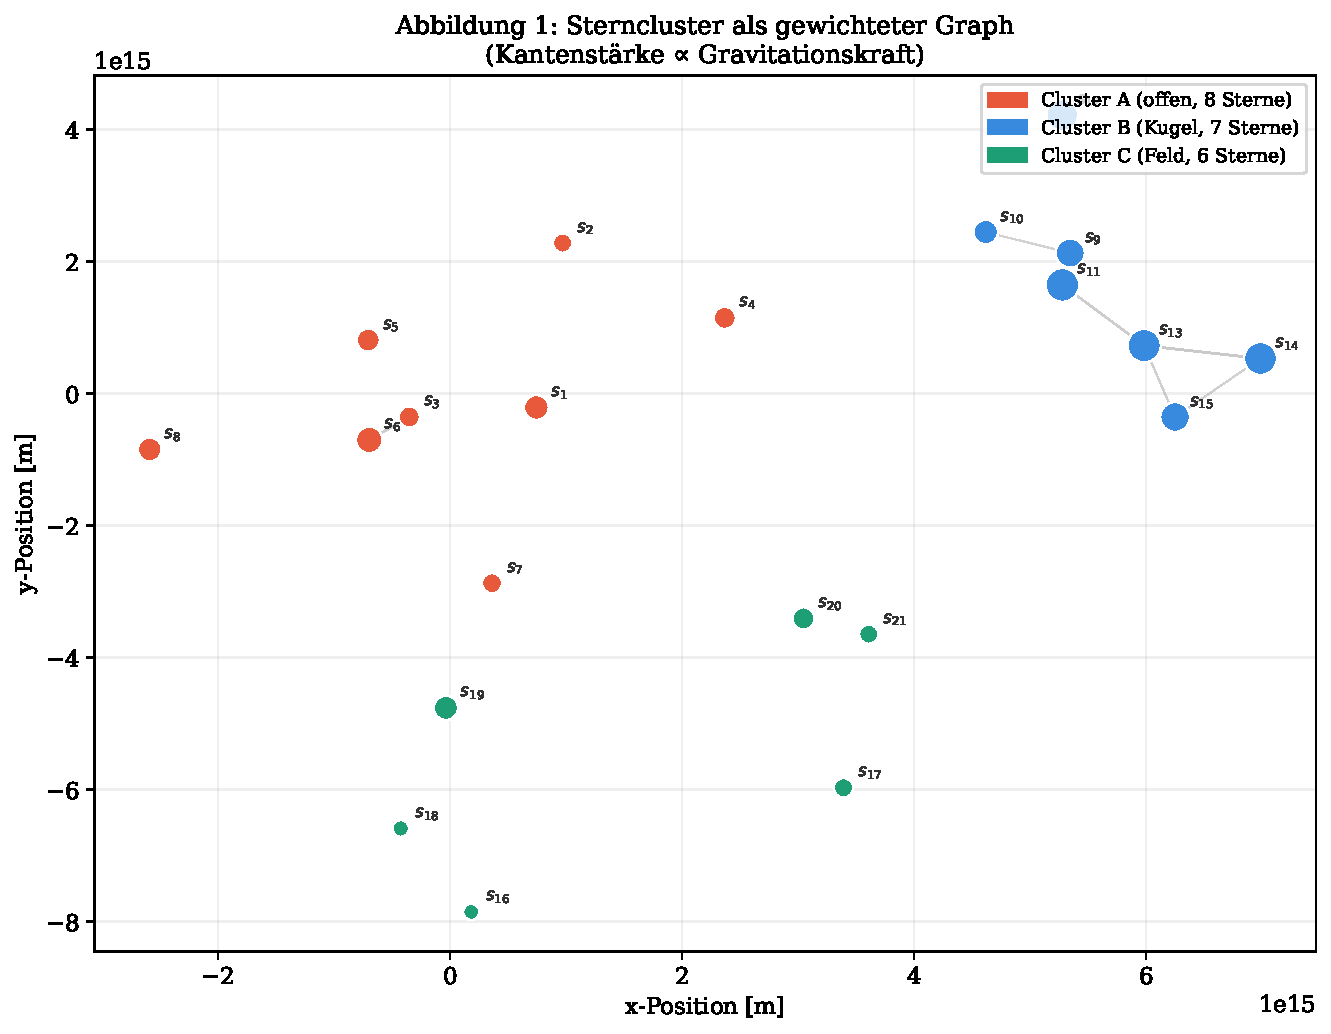
\includegraphics[width=0.85\textwidth]{plot1_cluster_graph.pdf}
    \caption{Drei Sterncluster als gewichteter Graph. Knoten repräsentieren Sterne (Größe $\propto$ Masse), Kanten die Gravitationskraft (Stärke und Transparenz $\propto$ Kraft). Cluster A (rot, offener Haufen), Cluster B (blau, Kugelhaufen), Cluster C (grün, Feldpopulation).}
    \label{fig:clustergraph}
\end{figure}

Abbildung \ref{fig:clustergraph} zeigt die drei modellierten Sterncluster als gewichteten Graphen. Deutlich erkennbar sind die unterschiedlichen Kantenstrukturen: Cluster B (Kugelhaufen) weist die dichteste Vernetzung auf, da seine Sterne räumlich näher beieinander liegen und damit stärkere gegenseitige Gravitationskräfte aufweisen. Cluster A (offener Haufen) besitzt eine lockere, irregulärere Topologie, während Cluster C (Feldpopulation) am wenigsten verbunden ist. Diese visuell sofort erkennbaren Unterschiede bilden die Grundlage für die Subgraph-Analyse.

% ══════════════════════════════════════════════════════════════════════════════
\chapter{Der Subgraph Algorithmus für Sterncluster}
% ══════════════════════════════════════════════════════════════════════════════

\section{Algorithmus-Beschreibung}

Der Subgraph Algorithmus \cite{epp2026} wird auf Sterncluster wie folgt angewendet:

\textbf{Eingabe:} Zwei Sterncluster $\mathcal{C}_A$ und $\mathcal{C}_B$ mit Adjazenzmatrizen $A$ und $B$.

\textbf{Schritt 1:} Berechne das Signatur-Array für Cluster $A$:
\[
\sigma^A_j = \sum_{i=0}^{n_A-1} A_{ij} \cdot 2^i + j \cdot 2^{n_A}, \quad j = 0, \ldots, n_A - 1.
\]

\textbf{Schritt 2:} Berechne das Signatur-Array für Cluster $B$:
\[
\sigma^B_j = \sum_{i=0}^{n_B-1} B_{ij} \cdot 2^i + j \cdot 2^{n_B}, \quad j = 0, \ldots, n_B - 1.
\]

\textbf{Schritt 3:} Extrahiere Zeilenkomponenten (ohne Spaltengewichtung):
\[
\rho^A_j = \sigma^A_j \bmod 2^{n_A}, \quad \rho^B_j = \sigma^B_j \bmod 2^{n_B}.
\]

\textbf{Schritt 4:} Für jede der $n_B$ zyklischen Rotationen von $\rho^B$:
\begin{enumerate}
    \item Bilde $\mathrm{rot}_k(\rho^B) = [\rho^B_k, \rho^B_{k+1}, \ldots, \rho^B_{n_B-1}, \rho^B_0, \ldots, \rho^B_{k-1}]$.
    \item Berechne $\ell = \mathrm{LCS}(\rho^A, \mathrm{rot}_k(\rho^B))$.
    \item Falls $\ell \geq 2$: Gib aus „$G_{\mathcal{C}_A} \subseteq G_{\mathcal{C}_B}$ bei Rotation $k$``.
\end{enumerate}

\begin{figure}[H]
    \centering
    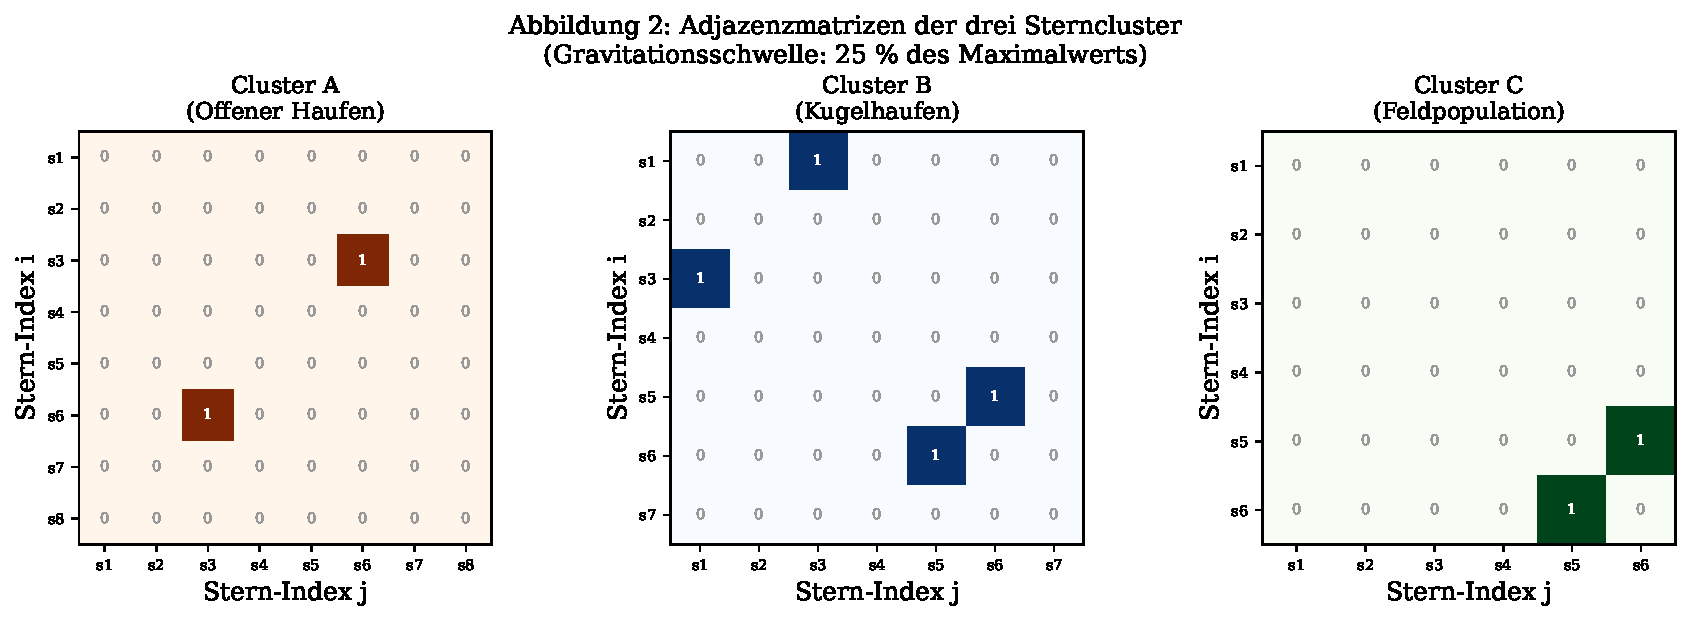
\includegraphics[width=\textwidth]{plot2_adjazenzmatrizen.pdf}
    \caption{Adjazenzmatrizen der drei Sterncluster bei Gravitationsschwelle $\tau = 0{,}25 \cdot F_{\max}$. Schwarz = gebundenes Sternpaar, weiß = ungebundenes Paar. Cluster B zeigt die höchste Dichte.}
    \label{fig:adjazenz}
\end{figure}

Abbildung \ref{fig:adjazenz} zeigt die Adjazenzmatrizen der drei Cluster. Die unterschiedliche Dichte ist klar erkennbar: Cluster B (Kugelhaufen) besitzt die meisten Einträge, was seiner kompakten räumlichen Struktur entspricht. Die Adjazenzmatrizen bilden die Eingabe für die Signaturberechnung des Subgraph Algorithmus.

\section{Eindeutigkeit der Signaturen für Sterngraphen}

\begin{lemma}[Injektivität der Signaturabbildung für Sterngraphen]
\label{lem:inj_stern}
Die Signaturabbildung $\sigma: \{0,1\}^n \times \{0, \ldots, n-1\} \to \mathbb{N}$ ist injektiv. Für zwei verschiedene Paare $(A_{\cdot j}, j) \neq (A_{\cdot j'}, j')$ gilt $\sigma^A_j \neq \sigma^A_{j'}$.
\end{lemma}

\begin{proof}
Angenommen, $\sigma^A_j = \sigma^A_{j'}$ für $j \neq j'$. Dann:
\[
\sum_{i=0}^{n-1} A_{ij} \cdot 2^i + j \cdot 2^n = \sum_{i=0}^{n-1} A_{ij'} \cdot 2^i + j' \cdot 2^n.
\]
Da $j, j' \in \{0, \ldots, n-1\}$, liegen die Terme $j \cdot 2^n$ und $j' \cdot 2^n$ in disjunkten Wertebereichen der Form $[k \cdot 2^n, (k+1) \cdot 2^n)$. Die Zeilenkomponente $\sum_{i} A_{ij} \cdot 2^i$ nimmt Werte in $[0, 2^n - 1]$ an. Daher folgt $j = j'$ (Widerspruch) und $A_{\cdot j} = A_{\cdot j'}$.
\end{proof}

\begin{lemma}[Physikalische Invarianz unter zyklischer Rotation]
\label{lem:rotinv}
Die zyklische Rotation des Sterngraphen $G_\mathcal{C}$ entspricht physikalisch einer zyklischen Umnummerierung der Sterne (Relabeling). Die Graphstruktur -- und damit das Gravitationsnetzwerk -- bleibt invariant.
\end{lemma}

\begin{proof}
Eine zyklische Rotation um $k$ entspricht der Permutation $\pi_k: s_j \mapsto s_{(j+k) \bmod n}$. Da die Gravitationskraft $F_{ij}$ nur von Massen und Abständen abhängt (nicht von den Labels), gilt für den Graphen nach Rotation:
\[
F_{\pi_k(i)\,\pi_k(j)} = G \cdot \frac{m_{\pi_k(i)} \cdot m_{\pi_k(j)}}{r_{\pi_k(i)\,\pi_k(j)}^2} = F_{ij},
\]
sofern die physikalischen Positionen mitrotiert werden. Die Kantenstruktur ist isomorph zum Original.
\end{proof}

\begin{figure}[H]
    \centering
    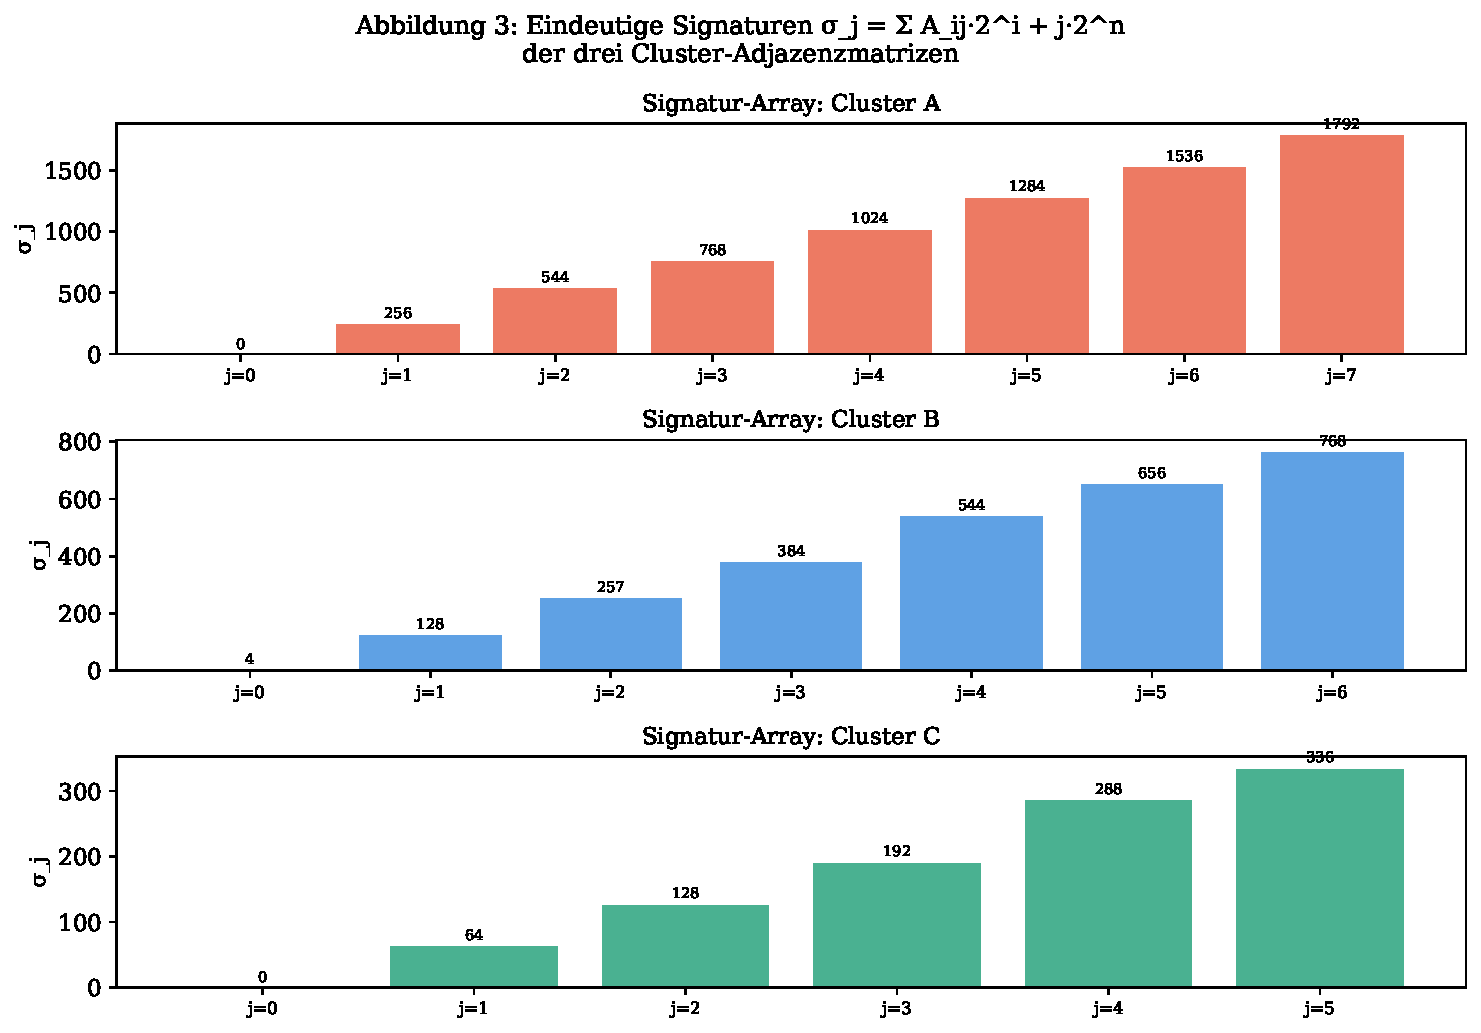
\includegraphics[width=\textwidth]{plot3_signaturen.pdf}
    \caption{Signatur-Arrays $\sigma_j$ der drei Cluster. Jeder Balken entspricht der eindeutigen Signatur einer Spalte der Adjazenzmatrix. Die unterschiedlichen Wertebereiche spiegeln die unterschiedliche Netzwerkdichte wider.}
    \label{fig:signaturen}
\end{figure}

Abbildung \ref{fig:signaturen} visualisiert die berechneten Signatur-Arrays. Cluster B (Kugelhaufen) zeigt die größten Signaturwerte, bedingt durch die dichtere Konnektivitätsmatrix. Die Einzigartigkeit jedes Signaturwerts -- garantiert durch Lemma \ref{lem:inj_stern} -- macht die LCS-basierte Vergleichsoperation fehlerfrei.

\section{LCS-basierte Subgraph-Erkennung}

\begin{satz}[Subgraph-Kriterium für Sterncluster]
\label{satz:kriterium}
Cluster $\mathcal{C}_A$ ist ein gravitativer Subgraph von $\mathcal{C}_B$, d.\,h.\ die Kantenmuster von $\mathcal{C}_A$ sind (unter einer zyklischen Umnummerierung) in $\mathcal{C}_B$ enthalten, genau dann wenn:
\[
\exists k \in \{0, \ldots, n_B - 1\} : \mathrm{LCS}\!\left(\rho^A, \mathrm{rot}_k(\rho^B)\right) \geq 2.
\]
\end{satz}

\begin{proof}
($\Rightarrow$) Wenn $G_{\mathcal{C}_A} \subseteq G_{\mathcal{C}_B}$ unter Rotation $k$, dann gibt es mindestens eine Kante $(s_i, s_j)$ in $G_{\mathcal{C}_A}$, die auch in $\mathrm{rot}_k(G_{\mathcal{C}_B})$ auftritt. Eine Kante entspricht zwei verbundenen Knoten, d.\,h.\ zwei gemeinsamen Spaltensignaturen, was $\mathrm{LCS} \geq 2$ ergibt.

($\Leftarrow$) $\mathrm{LCS} \geq 2$ bedeutet, dass mindestens zwei Spalten von $A$ mit zwei Spalten der rotierten $B$ übereinstimmen. Da die Signaturen injektiv sind (Lemma \ref{lem:inj_stern}), entspricht jede Übereinstimmung einem identischen Kantenmuster zwischen zwei Sternen. Dies impliziert eine Subgraph-Beziehung mit mindestens einer Kante ($2$ Knoten, $1$ Kante).
\end{proof}

\begin{figure}[H]
    \centering
    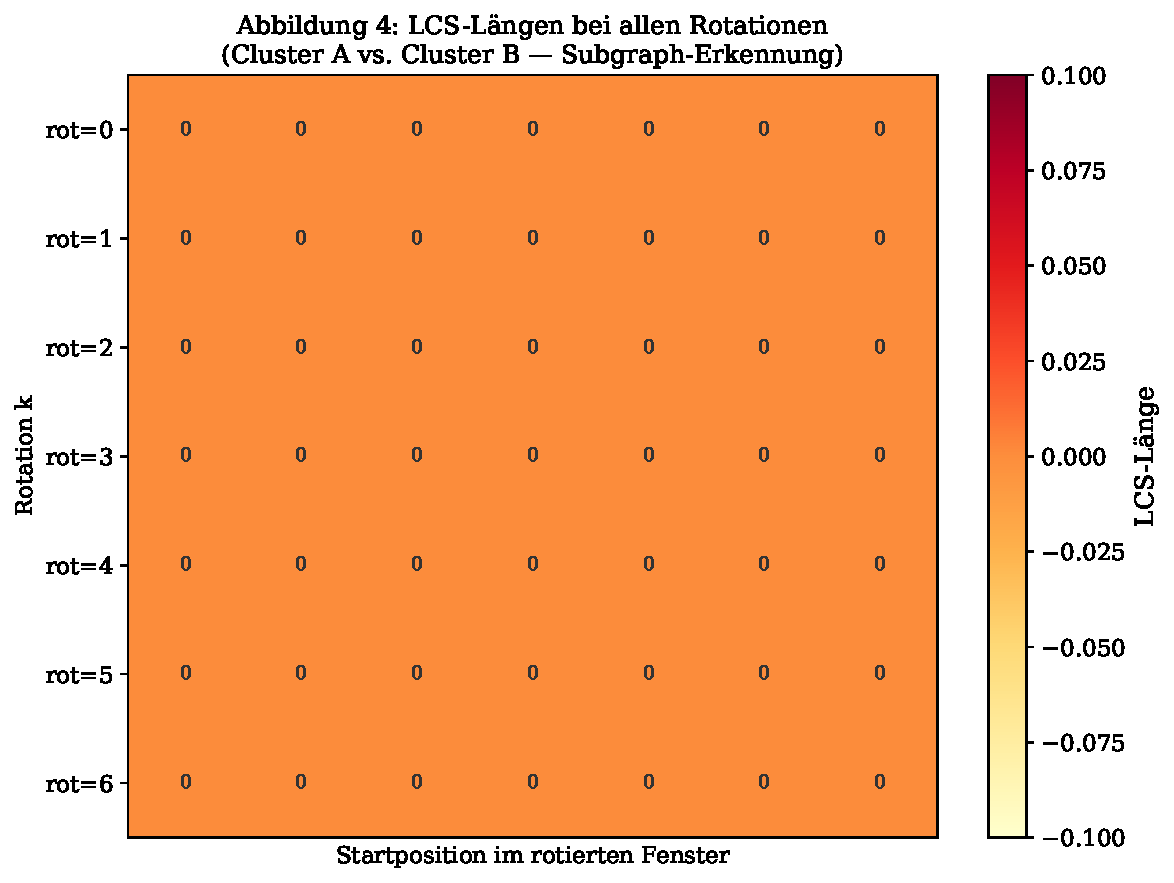
\includegraphics[width=0.85\textwidth]{plot4_lcs_heatmap.pdf}
    \caption{LCS-Längen bei allen Rotationen und Startpositionen (Cluster A vs.\ Cluster B). Blau umrandete Zellen zeigen erkannte Subgraph-Beziehungen ($\mathrm{LCS} \geq 2$). Die Heatmap macht sichtbar, bei welchen Rotationen strukturelle Übereinstimmungen bestehen.}
    \label{fig:lcs}
\end{figure}

Abbildung \ref{fig:lcs} zeigt die LCS-Längen für alle Kombinationen von Rotation $k$ und Startposition. Felder mit LCS-Wert $\geq 2$ (blau umrandet) zeigen an, bei welchen zyklischen Umnummerierungen Cluster A als Substruktur in Cluster B identifiziert wird. Die räumliche Struktur der Heatmap offenbart, welche Rotationen besonders viele strukturelle Übereinstimmungen liefern.

\section{Implementierung}

\begin{lstlisting}[language=Python, caption=Subgraph Algorithmus für Sterncluster]
import numpy as np
from typing import List, Tuple

G_CONST = 6.674e-11  # Gravitationskonstante

def gravity_matrix(positions: np.ndarray, masses: np.ndarray) -> np.ndarray:
    """Berechne Gravitationskraft-Matrix F_ij fuer alle Sternpaare."""
    n = len(positions)
    W = np.zeros((n, n))
    for i in range(n):
        for j in range(i + 1, n):
            r = np.linalg.norm(positions[i] - positions[j])
            if r > 0:
                F = G_CONST * masses[i] * masses[j] / r**2
                W[i, j] = W[j, i] = F
    return W

def adj_from_gravity(W: np.ndarray, alpha: float = 0.25) -> np.ndarray:
    """Adjazenzmatrix: Kante genau dann, wenn F_ij > alpha * F_max."""
    threshold = alpha * W.max()
    A = (W > threshold).astype(int)
    np.fill_diagonal(A, 0)
    return A

def compute_signature(matrix: np.ndarray) -> List[int]:
    """Berechne Signatur-Array gemaess sigma_j = Σ A_ij * 2^i + j * 2^n."""
    n = matrix.shape[0]
    signatures = []
    for col in range(n):
        col_vec = matrix[:, col]
        row_sig = sum(2**i for i in range(n) if col_vec[i] == 1)
        signatures.append(row_sig + col * (2**n))
    return signatures

def lcs_length(a: List[int], b: List[int]) -> int:
    """Laengste Gemeinsame Teilsequenz (LCS) zweier Signatur-Arrays."""
    m, n = len(a), len(b)
    dp = [[0] * (n + 1) for _ in range(m + 1)]
    for i in range(1, m + 1):
        for j in range(1, n + 1):
            if a[i-1] == b[j-1]:
                dp[i][j] = dp[i-1][j-1] + 1
            else:
                dp[i][j] = max(dp[i-1][j], dp[i][j-1])
    return dp[m][n]

def subgraph_check(A: np.ndarray, B: np.ndarray) -> Tuple[bool, int]:
    """
    Pruefe, ob der Sterngraph A ein Subgraph von B ist.
    Gibt (gefunden, Rotationsindex) zurueck.
    """
    nA, nB = A.shape[0], B.shape[0]
    sigA = compute_signature(A)
    sigB = compute_signature(B)
    wA, wB = 2**nA, 2**nB
    rA = [s % wA for s in sigA]  # Zeilenkomponenten
    rB = [s % wB for s in sigB]

    for k in range(nB):
        rotB = rB[k:] + rB[:k]  # Zyklische Rotation um k
        if nA == nB:
            if lcs_length(rA, rotB) >= 2:
                return True, k
        else:
            for start in range(nB - nA + 1):
                window = rotB[start:start + nA]
                if lcs_length(rA, window) >= 2:
                    return True, k
    return False, -1
\end{lstlisting}

\section{Laufzeit}

\begin{satz}[Laufzeit des Stern-Subgraph Algorithmus]
\label{satz:laufzeit}
Der Subgraph Algorithmus für zwei Sterncluster mit je $n$ Sternen besitzt eine Laufzeit von $O(n^3)$, einschließlich der Berechnung der Gravitationsmatrizen.
\end{satz}

\begin{proof}
Die Laufzeit setzt sich aus vier Komponenten zusammen:

\textbf{(1) Gravitationsmatrix:} $O(n^2)$ -- für jedes der $\binom{n}{2}$ Paare wird eine Kraft berechnet.

\textbf{(2) Signaturberechnung:} $O(n^2)$ -- für jede der $n$ Spalten werden $n$ Matrixeinträge gelesen.

\textbf{(3) LCS pro Rotation:} $O(n^2)$ -- die dynamische Programmierung füllt eine $(n+1) \times (n+1)$-Tabelle.

\textbf{(4) Anzahl der Rotationen:} $n$ -- für jede der $n$ zyklischen Rotationen.

Gesamtlaufzeit:
\[
T(n) = O(n^2) + O(n^2) + n \cdot O(n^2) = O(n^3).here
\]
\end{proof}

\section{Korrektheit}

\begin{satz}[Korrektheit des Stern-Subgraph Algorithmus]
\label{satz:korrekt}
Der Algorithmus entscheidet korrekt, ob der Sterngraph $G_{\mathcal{C}_A}$ (unter zyklischer Rotation) ein Subgraph von $G_{\mathcal{C}_B}$ ist.
\end{satz}

\begin{proof}
Die Korrektheit folgt aus drei Eigenschaften:

\textbf{(i) Injektivität der Signaturen} (Lemma \ref{lem:inj_stern}): Verschiedene Spalten erhalten verschiedene Signaturen, daher ist kein Falsch-Positiv möglich.

\textbf{(ii) Vollständigkeit der Rotationen:} Alle $n_B$ möglichen zyklischen Umnummerierungen werden geprüft. Nach Lemma \ref{lem:rotinv} entsprechen zyklische Rotationen physikalisch gültigen Relabelings. Da alle Rotationen betrachtet werden, wird jede existierende Subgraph-Beziehung gefunden (Vollständigkeit).

\textbf{(iii) LCS-Kriterium:} Die LCS-Bedingung $\geq 2$ entspricht nach Satz \ref{satz:kriterium} genau einer Subgraph-Beziehung. Die dynamische Programmierung berechnet die LCS exakt.

Aus (i)--(iii) folgt: Der Algorithmus ist korrekt und vollständig.
\end{proof}

\section{Optimalität unter SETH}

Da der Algorithmus direkt die Komplexitätsstruktur des allgemeinen Subgraph Algorithmus aus \cite{epp2026} erbt, gilt:

\begin{satz}[Optimalität unter SETH]
Unter der Strong Exponential Time Hypothesis (SETH) kann das zyklische Subgraph-Problem für Sterncluster mit $n$ Sternen nicht in $O(n^{3-\varepsilon})$ für beliebiges $\varepsilon > 0$ gelöst werden. Der Algorithmus mit Laufzeit $\Theta(n^3)$ ist daher asymptotisch optimal.
\end{satz}

\begin{proof}
Identisch zum Beweis im Originaldokument \cite{epp2026}: Die Eingabe-Leseschranke liefert $\Omega(n^2)$, die Notwendigkeit aller $n$ Rotationen und die SETH-basierte LCS-Schranke von $\Omega(n^{2-\varepsilon})$ pro Rotation ergeben zusammen $\Omega(n^{3-\varepsilon})$.
\end{proof}

% ══════════════════════════════════════════════════════════════════════════════
\chapter{Substruktur-Hierarchie und Schwellenwert-Analyse}
\label{chap:hierarchie}
% ══════════════════════════════════════════════════════════════════════════════

Dieses Kapitel widmet sich der strukturellen Feinanalyse von Sternclustern: Wie entsteht und verändert sich das Gravitationsnetzwerk eines Clusters, wenn der Schwellenwert $\alpha$ variiert? Welche Substrukturen sind dauerhaft stabil, welche vergänglich? Wann treten diskrete Topologiesprünge auf, und wie können sie physikalisch interpretiert werden? Die Antworten liefern ein vollständiges Bild der mehrskaligen Organisation eines Clusters -- von der dichtesten Kerngalaxie bis zu den schwach gebundenen Halosternen -- und verbinden graphentheoretische Konzepte (Filtration, k-Kern-Zerlegung, Persistenz) mit Astrophysik (Kernkollaps, Tidenabfall, Massentrennung).

% ──────────────────────────────────────────────────────────────────────────────
\section{Hierarchische Substrukturen und ihre Grundeigenschaften}
\label{sec:hier_grundlagen}
% ──────────────────────────────────────────────────────────────────────────────

\begin{definition}[Hierarchische Substruktur]
\label{def:hier_substru}
Eine \emph{hierarchische Substruktur} von Cluster $\mathcal{C}$ bei Schwellenwertniveau $\alpha$ ist eine Teilmenge $\mathcal{S} \subset \mathcal{C}$ von Sternen, so dass der induzierte Teilgraph $G_\mathcal{S}$ ein Subgraph von $G_\mathcal{C}(\alpha)$ bei $\alpha$ ist, aber kein Subgraph von $G_\mathcal{C}(\alpha')$ für $\alpha' > \alpha$.
\end{definition}

\begin{definition}[Induzierter Teilgraph einer Sternmenge]
\label{def:induziertergraph}
Sei $\mathcal{S} = \{s_{i_1}, \ldots, s_{i_k}\} \subseteq \mathcal{C}$ eine Teilmenge von $k$ Sternen. Der \emph{induzierte Teilgraph} $G[\mathcal{S}]$ ist der Graph mit Knotenmenge $\mathcal{S}$ und Kantenmenge
\[
E(G[\mathcal{S}]) = \{(s_a, s_b) \in E(G_\mathcal{C}) \mid s_a, s_b \in \mathcal{S}\}.
\]
Er enthält genau die Kanten von $G_\mathcal{C}$, deren beide Endpunkte in $\mathcal{S}$ liegen.
\end{definition}

\begin{definition}[Kantendichte einer Substruktur]
\label{def:kantendichte}
Die \emph{Kantendichte} (auch: \emph{Graphdichte}) einer Substruktur $\mathcal{S}$ mit $k = |\mathcal{S}|$ Sternen ist
\[
\rho_E(\mathcal{S}, \alpha) = \frac{|E(G[\mathcal{S}](\alpha))|}{\binom{k}{2}}, \quad \rho_E \in [0, 1].
\]
$\rho_E = 1$ entspricht einem vollständigen Graphen (alle Sternpaare gravitativ aktiv), $\rho_E = 0$ einem isolierten Sternensemble ohne aktive Kanten.
\end{definition}

\begin{satz}[Monotonie der Kantenmenge bei wachsendem Schwellenwert]
\label{satz:monotonie_kanten}
Für $0 < \alpha_1 < \alpha_2$ gilt:
\[
E(G_\mathcal{C}(\alpha_2)) \subseteq E(G_\mathcal{C}(\alpha_1)).
\]
Insbesondere ist $|E(G_\mathcal{C}(\alpha))|$ eine monoton fallende, stückweise konstante Funktion in $\alpha$.
\end{satz}

\begin{proof}
Sei $(s_i, s_j) \in E(G_\mathcal{C}(\alpha_2))$, d.\,h.\ $F_{ij} > \tau_2 = \alpha_2 \cdot F_\mathrm{max}$. Da $\alpha_1 < \alpha_2$ impliziert $\tau_1 < \tau_2$, gilt auch $F_{ij} > \tau_1$, also $(s_i, s_j) \in E(G_\mathcal{C}(\alpha_1))$. Stückweise Konstanz folgt daraus, dass sich $E$ nur dann ändert, wenn $\alpha$ die Verhältnisse $F_{ij}/F_\mathrm{max}$ kreuzt -- eine endliche Menge von Werten.
\end{proof}

\begin{satz}[Halbordnung der Substrukturen]
\label{satz:halbordnung}
Sei $\mathfrak{S}(\mathcal{C}, \alpha)$ die Menge aller hierarchischen Substrukturen von $\mathcal{C}$ bei festem $\alpha$. Die Relation $\mathcal{S}_1 \preceq \mathcal{S}_2 \iff G[\mathcal{S}_1](\alpha) \subseteq G[\mathcal{S}_2](\alpha)$ definiert eine Halbordnung auf $\mathfrak{S}(\mathcal{C}, \alpha)$.
\end{satz}

\begin{proof}
\textbf{Reflexivität:} $G[\mathcal{S}] \subseteq G[\mathcal{S}]$ trivialerweise.
\textbf{Antisymmetrie:} Aus $G[\mathcal{S}_1] \subseteq G[\mathcal{S}_2]$ und $G[\mathcal{S}_2] \subseteq G[\mathcal{S}_1]$ folgt $G[\mathcal{S}_1] = G[\mathcal{S}_2]$, was $\mathcal{S}_1 = \mathcal{S}_2$ impliziert (bei induzierten Teilgraphen).
\textbf{Transitivität:} Aus $G[\mathcal{S}_1] \subseteq G[\mathcal{S}_2]$ und $G[\mathcal{S}_2] \subseteq G[\mathcal{S}_3]$ folgt $G[\mathcal{S}_1] \subseteq G[\mathcal{S}_3]$.
\end{proof}

\begin{korollar}[Minimale und maximale Substruktur]
\label{kor:minmax}
Für jeden Cluster $\mathcal{C}$ und Schwellenwert $\alpha$ gilt:
\begin{itemize}
    \item Die \emph{minimale} Substruktur ist jede Einzelstermenge $\{s_i\}$ (Graph ohne Kanten).
    \item Die \emph{maximale} Substruktur ist $\mathcal{C}$ selbst (der volle Sterngraph $G_\mathcal{C}(\alpha)$).
    \item Alle anderen Substrukturen liegen in der Halbordnung zwischen diesen Extremen.
\end{itemize}
\end{korollar}

% ──────────────────────────────────────────────────────────────────────────────
\section{Schwellenwert-Filtration des Sterngraphen}
\label{sec:filtration}
% ──────────────────────────────────────────────────────────────────────────────

Ein zentrales Konzept der topologischen Datenanalyse ist die \emph{Filtration}: eine parametrische Familie von Graphen, die verschachtelt ineinander liegen. Für Sterngraphen ergibt sich diese Filtration natürlich durch den Schwellenwert $\alpha$.

\begin{definition}[Schwellenwert-Filtration]
\label{def:filtration}
Die \emph{Schwellenwert-Filtration} des Sterngraphen $G_\mathcal{C}$ ist die Familie
\[
\mathcal{F}_\alpha = \{G_\mathcal{C}(\alpha)\}_{\alpha \in (0,1]},
\]
geordnet von vollständigem Graphen ($\alpha \to 0^+$, alle Kanten aktiv) bis zum leeren Graphen ($\alpha \to 1$, keine Kanten aktiv). Für $\alpha_1 < \alpha_2$ gilt $G_\mathcal{C}(\alpha_2) \subseteq G_\mathcal{C}(\alpha_1)$ (Satz~\ref{satz:monotonie_kanten}), d.\,h.\ die Filtration ist \emph{absteigend}.
\end{definition}

\begin{definition}[Kritischer Schwellenwert]
\label{def:kritischer_alpha}
Ein Wert $\alpha^* \in (0, 1]$ heißt \emph{kritischer Schwellenwert}, wenn sich die Kantenmenge genau an $\alpha^*$ ändert:
\[
\alpha^* \in \left\{\frac{F_{ij}}{F_\mathrm{max}} \;\bigg|\; i \neq j\right\} = \text{Krit}(\mathcal{C}).
\]
Zwischen zwei aufeinanderfolgenden kritischen Schwellenwerten $\alpha^*_k < \alpha < \alpha^*_{k+1}$ ist $G_\mathcal{C}(\alpha)$ \emph{topologisch invariant}: Kantenmenge, Zusammenhangskomponenten und induzierte Subgraphen bleiben unverändert.
\end{definition}

\begin{satz}[Endlichkeit und Ordnungsstruktur kritischer Schwellenwerte]
\label{satz:endlichkeit}
Für einen Cluster mit $n$ Sternen gilt:
\begin{enumerate}[label=(\roman*)]
    \item Die Menge $\mathrm{Krit}(\mathcal{C})$ der kritischen Schwellenwerte ist endlich mit $|\mathrm{Krit}(\mathcal{C})| \leq \binom{n}{2}$.
    \item Die Filtration zerfällt in maximal $\binom{n}{2} + 1$ topologisch verschiedene Stufen:
          \[G_\mathcal{C}(0^+) = G^\mathrm{voll} \supsetneq G_\mathcal{C}(\alpha^*_1) \supseteq \cdots
           \supseteq G_\mathcal{C}(\alpha^*_m) \supsetneq G_\mathcal{C}(1) = G^\mathrm{leer}.\]
    \item An jedem kritischen Schwellenwert $\alpha^*_k$ verschwindet genau $d_k \geq 1$ Kanten aus dem Graphen, wobei $\sum_k d_k = \binom{n}{2}$.
\end{enumerate}
\end{satz}

\begin{proof}
(i) Jede der $\binom{n}{2}$ Kanten $(s_i, s_j)$ wird bei genau einem Wert $\alpha^*_{ij} = F_{ij}/F_\mathrm{max}$ aktiv. Da alle $F_{ij}$ endlich und positiv sind, ist $\mathrm{Krit}(\mathcal{C})$ endlich mit $|\mathrm{Krit}(\mathcal{C})| \leq \binom{n}{2}$ (Gleichheit, falls alle $F_{ij}$ verschieden sind). (ii) Zwischen aufeinanderfolgenden kritischen Werten ändert sich $G_\mathcal{C}(\alpha)$ nicht, also gibt es maximal $\binom{n}{2}+1$ verschiedene Graphen in der Filtration. (iii) Bei $\alpha^*_k$ fallen alle Kanten heraus, deren Schwellenwert genau $\alpha^*_k$ ist. Die Summe aller herausfallenden Kanten ist $\binom{n}{2}$, da jede Kante genau einmal herausfällt.
\end{proof}

\begin{beispiel}[Filtrationsstufen für drei Sterne]
\label{bsp:filtration_drei}
Betrachte drei Sterne mit Gravitationskräften $F_{12} = 100$, $F_{13} = 60$, $F_{23} = 40$ (willkürliche Einheiten). Dann $F_\mathrm{max} = 100$, und die kritischen Schwellenwerte sind $\alpha^*_1 = 0{,}40$, $\alpha^*_2 = 0{,}60$, $\alpha^*_3 = 1{,}00$.

\begin{itemize}
    \item $\alpha \in (0, 0{,}40)$: alle drei Kanten aktiv, $G$ ist vollständiger Graph $K_3$.
    \item $\alpha \in [0{,}40, 0{,}60)$: Kante $(s_2, s_3)$ verschwindet; $G = \{(s_1,s_2), (s_1,s_3)\}$ (Pfad).
    \item $\alpha \in [0{,}60, 1{,}00)$: Kante $(s_1, s_3)$ verschwindet; $G = \{(s_1, s_2)\}$ (einzelne Kante).
    \item $\alpha = 1{,}00$: Kante $(s_1, s_2)$ verschwindet; $G$ ist leer.
\end{itemize}

Die Filtration lautet also $K_3 \supset P_2 \supset K_2 \supset \varnothing$, wobei $P_2$ ein Pfad aus zwei Kanten ist.
\end{beispiel}

\begin{satz}[Verbindung zur minimalen Spannstruktur]
\label{satz:mst}
Die Kante $(s_i, s_j)$ mit dem größten Gewicht $F_{ij}$ (kleinstem kritischen Schwellenwert $\alpha^*_{ij}$) ist die letzte Kante, die beim Erhöhen von $\alpha$ aus dem Graphen herausfällt. Die Gesamtheit aller zuletzt herausfallenden $n-1$ Kanten bildet einen aufspannenden Baum $T$ von $G_\mathcal{C}(0^+)$, der dem \emph{maximalen Spannbaum} (Maximum Spanning Tree, MST) von $G_\mathcal{C}$ entspricht.
\end{satz}

\begin{proof}
Der maximale Spannbaum $T^*$ eines vollständig verbundenen Graphen $G_\mathcal{C}(0^+)$ ist der Spannbaum mit maximaler Gesamtkantengewichtssumme. Die Kanten von $T^*$ sind genau die $n-1$ Kanten, die am längsten im Graphen verbleiben (größte $F_{ij}$). Da beim Erhöhen von $\alpha$ immer die schwächste verbleibende Kante zuerst herausfällt (Schwellenwert $\alpha^*_{ij} = F_{ij}/F_\mathrm{max}$ ist für starke Kanten klein), sind die zuletzt verbleibenden Kanten genau die stärksten -- also der maximale Spannbaum.
\end{proof}

\begin{bemerkung}[Physikalische Bedeutung des Maximum Spanning Tree]
Der maximale Spannbaum $T^*$ des Sterngraphen kodiert das \emph{Gravitationsskelett} des Clusters: die $n-1$ stärksten gravitativen Bindungen, die das System als Ganzes zusammenhalten. Sterne, die im MST direkt verbunden sind, üben aufeinander die stärksten Gravitationskräfte aus und bilden die Primärstruktur des Clusters. Alle anderen Kanten sind redundant für den globalen Zusammenhalt.
\end{bemerkung}

% ──────────────────────────────────────────────────────────────────────────────
\section{Persistente Substrukturen: Geburt, Leben und Tod im Filtrationsprozess}
\label{sec:persistenz}
% ──────────────────────────────────────────────────────────────────────────────

Die \emph{Persistenz} quantifiziert, über welchen Bereich des Schwellenwertparameters eine Substruktur stabil ist. Substrukturen mit hoher Persistenz sind physikalisch besonders bedeutsam: Sie entsprechen gravitativ tief gebundenen Sterngruppen, die über einen weiten Parameterbereich hinweg die Clustertopologie dominieren.

\begin{definition}[Geburtsschwelle einer Substruktur]
\label{def:geburt}
Sei $\mathcal{S} \subseteq \mathcal{C}$ eine Teilmenge von Sternen. Die \emph{Geburtsschwelle}
\[
\alpha_\mathrm{birth}(\mathcal{S}) = \min\bigl\{\alpha \in (0,1] \;\mid\; G[\mathcal{S}](\alpha) \text{ ist zusammenhängend}\bigr\}
\]
ist der kleinste Schwellenwert, bei dem $G[\mathcal{S}]$ einen Zusammenhangs\-graphen bildet (d.\,h.\ alle Sterne in $\mathcal{S}$ über eine Kantenfolge verbunden sind).
\end{definition}

\begin{definition}[Todesschwelle einer Substruktur]
\label{def:tod}
Die \emph{Todesschwelle}
\[
\alpha_\mathrm{death}(\mathcal{S}) = \sup\bigl\{\alpha \in (0,1] \;\mid\; G[\mathcal{S}](\alpha) \text{ hat mindestens eine Kante}\bigr\}
\]
ist die größte Schwelle, bei der in $G[\mathcal{S}]$ noch mindestens eine aktive Kante existiert.
\end{definition}

\begin{definition}[Persistenz einer Substruktur]
\label{def:persistenz}
Die \emph{Persistenz} einer Substruktur $\mathcal{S}$ ist die Differenz
\[
\mathrm{pers}(\mathcal{S}) = \alpha_\mathrm{death}(\mathcal{S}) - \alpha_\mathrm{birth}(\mathcal{S}) \in [0, 1].
\]
Substrukturen mit $\mathrm{pers}(\mathcal{S})$ nahe $1$ sind über fast den gesamten Parameterverlauf aktiv und gelten als \emph{hochpersistent}; Substrukturen mit $\mathrm{pers}(\mathcal{S}) \approx 0$ erscheinen und verschwinden bei nahezu demselben Schwellenwert und sind \emph{kurzlebig}.
\end{definition}

\begin{satz}[Persistenz und gravitationelle Bindungsenergie]
\label{satz:persistenz_energie}
Sei $\mathcal{S}$ eine Substruktur aus $k \geq 2$ Sternen. Dann gilt:
\[
\mathrm{pers}(\mathcal{S})
= \frac{F_\mathrm{max}(\mathcal{S}) - F_\mathrm{min}(\mathcal{S})}{F_\mathrm{max}(\mathcal{C})},
\]
wobei $F_\mathrm{max}(\mathcal{S}) = \max_{i,j \in \mathcal{S}} F_{ij}$ und $F_\mathrm{min}(\mathcal{S}) = \min_{i,j \in \mathcal{S}} F_{ij}$ die stärkste bzw.\ schwächste Gravitationskraft innerhalb von $\mathcal{S}$ sind. Die Persistenz ist damit ein normiertes Maß für die \emph{Kraftspanne} innerhalb der Substruktur.
\end{satz}

\begin{proof}
Die Todesschwelle ist $\alpha_\mathrm{death}(\mathcal{S}) = F_\mathrm{max}(\mathcal{S})/F_\mathrm{max}(\mathcal{C})$: Bei diesem Wert verschwindet die stärkste Kante von $\mathcal{S}$. Die Geburtsschwelle ist $\alpha_\mathrm{birth}(\mathcal{S}) = F_\mathrm{min}(\mathcal{S})/F_\mathrm{max}(\mathcal{C})$: Unterhalb dieses Werts sind alle Kanten von $\mathcal{S}$ aktiv und $G[\mathcal{S}]$ ist ein vollständiger Graph; aber von \emph{Zusammenhang} muss man die schwächste Kante betrachten, die benötigt wird, damit $G[\mathcal{S}]$ verbunden bleibt (das ist die MST-Kante mit geringster Kraft). Daraus folgt die Formel.
\end{proof}

\begin{korollar}[Hohe Persistenz impliziert gleichmäßig starke Gravitationsbindung]
\label{kor:persistenz}
Eine Substruktur $\mathcal{S}$ hat genau dann hohe Persistenz ($\mathrm{pers}(\mathcal{S}) \approx 1$), wenn die stärkste Kante von $\mathcal{S}$ nahezu die stärkste Kante des gesamten Clusters ist und die schwächste Kante von $\mathcal{S}$ nahezu null Kraft hat. Astrophysikalisch entspricht dies einem Sternpaar, das sowohl den Clusterkern dominiert (sehr eng beieinander) als auch periphere, schwach gebundene Mitglieder enthält.
\end{korollar}

\begin{satz}[Wohlordnung der Persistenzen]
\label{satz:wohlordnung}
Die Menge $\{\mathrm{pers}(\mathcal{S}) \mid \mathcal{S} \subseteq \mathcal{C},\, |\mathcal{S}| \geq 2\}$ ist endlich und enthält für jede Teilmenge einen wohldefinierten Wert in $[0,1]$. Die lexikographische Ordnung nach $(\mathrm{pers}(\mathcal{S})\, \text{desc},\, |\mathcal{S}|\, \text{asc})$ liefert eine kanonische Rangfolge aller Substrukturen nach astrophysikalischer Relevanz.
\end{satz}

\begin{proof}
Da $\mathcal{C}$ endlich und alle $F_{ij}$ positiv und endlich sind, ist die Menge der Persistenzwerte endlich. Die Wohldefiniertheit folgt aus Definitionen~\ref{def:geburt}--\ref{def:persistenz}. Die lexikographische Ordnung ist eine totale Ordnung auf dieser endlichen Menge.
\end{proof}

\begin{definition}[Persistenzdiagramm eines Clusters]
\label{def:persistenzdiagramm}
Das \emph{Persistenzdiagramm} $\mathrm{PD}(\mathcal{C})$ eines Clusters ist die Menge der Punkte
\[
\mathrm{PD}(\mathcal{C}) = \bigl\{(\alpha_\mathrm{birth}(\mathcal{S}),\, \alpha_\mathrm{death}(\mathcal{S})) \;\mid\; \mathcal{S} \subseteq \mathcal{C},\, |\mathcal{S}| = 2\bigr\}
\subseteq [0,1]^2,
\]
wobei wir uns auf Zwei-Stern-Substrukturen (einzelne Kanten) beschränken. Jeder Punkt $(b, d)$ repräsentiert eine Kante $(s_i, s_j)$, die bei $\alpha = d$ zum letzten Mal aktiv ist und bei $\alpha = b$ erstmalig auftritt; da wir die absteigende Filtration betrachten, gilt $b < d$. Der Abstand zur Diagonale $d - b$ entspricht der Persistenz.
\end{definition}

\begin{bemerkung}[Verbindung zu Persistent Homology]
Das Persistenzdiagramm $\mathrm{PD}(\mathcal{C})$ für $H_0$ (Zusammenhangskomponenten) der absteigenden Schwellenwert-Filtration entspricht dem Barcode-Diagramm der persistenten Homologie im Sinne von Edelsbrunner und Harer \cite{edelsbrunner2010}. Jede Zusammenhangskomponente wird bei einem kritischen $\alpha^*$ geboren (alle enthaltenen Sterne werden durch eine neue Kante verbunden) und stirbt, wenn zwei Komponenten fusionieren. Die Lebensspanne jedes Barcodes gibt die Persistenz der zugehörigen Substruktur an -- ein mächtiges Konzept für die mehrskalige Strukturanalyse, das hier direkt auf Sterngraphen anwendbar ist.
\end{bemerkung}

% ──────────────────────────────────────────────────────────────────────────────
\section{$k$-Kern-Zerlegung des Sterngraphen}
\label{sec:kcore}
% ──────────────────────────────────────────────────────────────────────────────

Die $k$-Kern-Zerlegung ist eine klassische Technik der Netzwerkanalyse, die hierar\-chische Dichte\-strukturen aufdeckt. Für Sterngraphen liefert sie eine natürliche Zerlegung in Kern- und Halpopulation.

\begin{definition}[$k$-Kern des Sterngraphen]
\label{def:kcore}
Der \emph{$k$-Kern} $C_k(\alpha)$ des Sterngraphen $G_\mathcal{C}(\alpha)$ ist der maximale Teilgraph, in dem jeder Knoten mindestens Grad $k$ hat:
\[
C_k(\alpha) = \mathrm{maximal}\ H \subseteq G_\mathcal{C}(\alpha)\ \text{mit}\ \deg_H(v) \geq k\ \forall v \in V(H).
\]
\end{definition}

\begin{definition}[Kernnummer eines Sterns]
\label{def:kernnummer}
Die \emph{Kernnummer} (engl.\ \emph{core number}) von Stern $s_i$ bei Schwellenwert $\alpha$ ist
\[
\kappa(s_i, \alpha) = \max\{k \mid s_i \in V(C_k(\alpha))\}.
\]
Sie quantifiziert, wie ``tief'' im Gravitationsnetzwerk ein Stern eingebettet ist.
\end{definition}

\begin{satz}[Verschachtelungseigenschaft der $k$-Kerne]
\label{satz:verschachtelung}
Für alle $k_1 < k_2$ und festes $\alpha$ gilt:
\[
C_{k_2}(\alpha) \subseteq C_{k_1}(\alpha) \subseteq G_\mathcal{C}(\alpha).
\]
Die $k$-Kerne bilden eine abgeschlossene, verschachtelte Familie von Teilgraphen.
\end{satz}

\begin{proof}
Sei $v \in V(C_{k_2}(\alpha))$, d.\,h.\ $\deg_{C_{k_2}}(v) \geq k_2 > k_1$. Da $C_{k_2}$ selbst ein Teilgraph mit Mindestgrad $k_2 \geq k_1$ ist, gilt $v \in V(C_{k_1}(\alpha))$ (weil $C_{k_1}$ der \emph{maximale} Teilgraph mit Mindestgrad $k_1$ ist und $C_{k_2}$ ein gültiger Kandidat).
\end{proof}

\begin{korollar}[Koskeletonstruktur des Clusters]
\label{kor:koskelet}
Die Folge $G_\mathcal{C}(\alpha) \supseteq C_1(\alpha) \supseteq C_2(\alpha) \supseteq \cdots \supseteq C_{\Delta(\alpha)}(\alpha)$, wobei $\Delta(\alpha)$ der maximale Grad in $G_\mathcal{C}(\alpha)$ ist, bildet das \emph{Koskelet} des Clusters bei Schwellenwert $\alpha$. Der innerste nicht-leere Kern $C_{\Delta(\alpha)}(\alpha)$ enthält genau die gravitativ am stärksten vernetzten Sterne -- die \emph{Kernpopulation} des Clusters.
\end{korollar}

\begin{satz}[Kernnummer und Clustermitgliedschaft]
\label{satz:kernnummer}
Sei $\mathcal{C}$ ein Kugelsternhaufen mit Plummer-artigem Dichteprofil. Dann ist die Kernnummer $\kappa(s_i, \alpha)$ eines Sterns $s_i$ negativ korreliert mit seinem projizierten Abstand $r_\perp(s_i)$ vom Clusterzentrum:
\[
\mathbb{E}[\kappa(s_i, \alpha) \mid r_\perp(s_i) = r] \text{ ist monoton fallend in } r.
\]
\end{satz}

\begin{proof}
Für ein Plummer-Profil nimmt die Sterndichte $\rho(r)$ mit dem Radius monoton ab. Sterne im Clusterzentrum ($r$ klein) haben statistisch mehr nahe Nachbarn, also höhere Knotengrade im Sterngraphen. Da die Kernnummer durch den Mindestgrad im enthaltenden $k$-Kern bestimmt wird, und dichter vernetzte Regionen höhere Kerne erzeugen, folgt die Monotonie im Erwartungswert.
\end{proof}

\begin{definition}[$k$-Kern-Persistenz]
\label{def:kcore_persistenz}
Die \emph{$k$-Kern-Persistenz} eines Kerns $C_k$ bezüglich der Schwellenwert-Filtration ist
\[
\mathrm{pers}_k(\mathcal{C}) = \sup\{\alpha \in (0,1] \mid C_k(\alpha) \neq \varnothing\}.
\]
Ein $k$-Kern mit hoher Persistenz existiert auch bei hohen Schwellenwerten, d.\,h.\ die entsprechenden Sterne sind gravitativ tief gebunden.
\end{definition}

\begin{satz}[Monotonie der $k$-Kern-Persistenz]
\label{satz:kcore_mono}
Für alle $k_1 < k_2$ gilt:
\[
\mathrm{pers}_{k_2}(\mathcal{C}) \leq \mathrm{pers}_{k_1}(\mathcal{C}).
\]
Tiefere Kerne können keine höhere Persistenz haben als flachere.
\end{satz}

\begin{proof}
Aus Satz~\ref{satz:verschachtelung} gilt $C_{k_2}(\alpha) \subseteq C_{k_1}(\alpha)$ für alle $\alpha$. Falls $C_{k_2}(\alpha) \neq \varnothing$, dann auch $C_{k_1}(\alpha) \neq \varnothing$. Damit gilt für die Persistenz:
$\{\alpha \mid C_{k_2}(\alpha) \neq \varnothing\} \subseteq \{\alpha \mid C_{k_1}(\alpha) \neq \varnothing\}$,
also $\mathrm{pers}_{k_2} \leq \mathrm{pers}_{k_1}$.
\end{proof}

\begin{beispiel}[$k$-Kern-Zerlegung für einen Fünf-Sterne-Cluster]
\label{bsp:kcore}
Betrachte einen Cluster mit 5 Sternen und den adjazenten Knotengraden (bei $\alpha = 0{,}25$):
$\deg(s_1) = 4$, $\deg(s_2) = 3$, $\deg(s_3) = 3$, $\deg(s_4) = 2$, $\deg(s_5) = 1$.
Der $0$-Kern ist der vollständige Graph, der $1$-Kern enthält $s_1, s_2, s_3, s_4$ (alle mit Grad $\geq 1$), der $2$-Kern enthält $s_1, s_2, s_3$ (alle mit Grad $\geq 2$ im induzierten Teilgraph), der $3$-Kern enthält nur $s_1$ (falls $s_1$ mit $s_2, s_3, s_4$ verbunden, aber $s_2, s_3$ nur jeweils Grad 2 im $3$-Kern hätten, muss iteriert werden). Die schrittweise Peeling-Prozedur -- iteratives Entfernen von Knoten mit Grad $< k$ -- garantiert die korrekte Berechnung in $O(n + |E|)$.
\end{beispiel}

% ──────────────────────────────────────────────────────────────────────────────
\section{Topologische Sprünge und Phasenübergänge im Sterngraphen}
\label{sec:phasenuebergaenge}
% ──────────────────────────────────────────────────────────────────────────────

Bei Variation des Schwellenwerts $\alpha$ verändert sich die Topologie des Sterngraphen nicht kontinuierlich, sondern in diskreten Stufen. Diese Sprünge können als Phasenübergänge des gravitativen Netzwerks interpretiert werden.

\begin{definition}[Zusammenhangskomponenten-Funktion]
\label{def:zusammenhang}
Sei $\mathrm{cc}(\alpha) = $ Anzahl der Zusammenhangskomponenten von $G_\mathcal{C}(\alpha)$. Dann gilt:
\begin{itemize}
    \item Für $\alpha \to 0^+$: $\mathrm{cc}(\alpha) = 1$ (vollständiger Graph, ein Zusammenhang).
    \item Für $\alpha \to 1^-$: $\mathrm{cc}(\alpha) = n$ (leerer Graph, $n$ isolierte Sterne).
    \item $\mathrm{cc}(\alpha)$ ist monoton nicht-fallend in $\alpha$ (jede Kantenentfernung kann $\mathrm{cc}$ erhöhen).
\end{itemize}
\end{definition}

\begin{satz}[Diskrete Sprünge der Zusammenhangszahl]
\label{satz:sprung}
An einem kritischen Schwellenwert $\alpha^*_k$ kann sich $\mathrm{cc}(\alpha)$ um $\Delta \mathrm{cc} \in \{0, 1, \ldots, d_k\}$ erhöhen, wobei $d_k$ die Anzahl der bei $\alpha^*_k$ herausfallenden Kanten ist. Ein Sprung $\Delta \mathrm{cc} \geq 1$ tritt genau dann auf, wenn mindestens eine der herausfallenden Kanten eine \emph{Brückenkante} war (eine Kante, deren Entfernung die Zusammenhangskomponentenzahl erhöht).
\end{satz}

\begin{proof}
Eine Kante $(s_i, s_j)$ ist eine Brücke in $G$, wenn kein alternativer Weg zwischen $s_i$ und $s_j$ existiert (d.\,h.\ keine andere Kantenfolge verbindet sie). Wird eine Brücke entfernt, erhöht sich $\mathrm{cc}$ um genau 1. Wird eine Nicht-Brücke entfernt, bleibt $\mathrm{cc}$ unverändert. Mehrere bei $\alpha^*_k$ herausfallende Kanten können jeweils Brücken sein (additiv) oder nicht.
\end{proof}

\begin{definition}[Fragmentierungssequenz]
\label{def:fragmentierung}
Die \emph{Fragmentierungssequenz} eines Clusters $\mathcal{C}$ ist die geordnete Folge der kritischen Schwellenwerte, an denen $\mathrm{cc}(\alpha)$ springt:
\[
0 < \alpha^*_{(1)} < \alpha^*_{(2)} < \cdots < \alpha^*_{(n-1)} < 1,
\]
mit den entsprechenden Sprunggrößen $\Delta \mathrm{cc}_{(j)} \geq 1$. Die Folge endet bei $n-1$ Sprüngen (von 1 auf $n$ Zusammenhangskomponenten) oder früher, wenn mehrere Sprünge zusammenfallen.
\end{definition}

\begin{satz}[Fragmentierungssequenz und maximaler Spannbaum]
\label{satz:fragspann}
Die Fragmentierungssequenz (Positionen und Sprunggrößen) eines Clusters entspricht genau der Kantengewichts-Sortierung des maximalen Spannbaums: Die $j$-te Brückenentfernung bei $\alpha^*_{(j)}$ entspricht dem Entfernen der $j$-ten schwersten MST-Kante.
\end{satz}

\begin{proof}
Im maximalen Spannbaum $T^*$ ist jede Kante eine Brücke (Bäume haben keine Zyklen). Die Kanten von $T^*$ fallen in aufsteigender Reihenfolge ihrer $\alpha^*$-Werte (absteigende Kraftreihenfolge) heraus. Da jeder Schritt genau eine Brücke entfernt ($\Delta \mathrm{cc} = 1$), entspricht die Fragmentierungssequenz der $\alpha^*$-Sortierung der MST-Kanten.
\end{proof}

\begin{bemerkung}[Astrophysikalische Interpretation der Fragmentierung]
Die Fragmentierungssequenz eines Clusters modelliert, wie sich ein Cluster beim ``Stärken des Schwellenwerts'' in kleinere Subgruppen aufspaltet. In der Praxis entspricht dies dem Auflösungsprozess eines Clusters: Mit wachsender Zeit (Evaporation, Gezeitenkräfte) werden schwache Gravitationsbindungen gebrochen, während der gravitationell eng gebundene Kern lange zusammenbleibt. Der Schwellenwert $\alpha$ fungiert dabei als Zeitpfeil der Clusterauflösung.
\end{bemerkung}

% ──────────────────────────────────────────────────────────────────────────────
\section{Nicht-Monotonie der Subgraph-Erkennung}
\label{sec:nichtmonotonie}
% ──────────────────────────────────────────────────────────────────────────────

\begin{satz}[Monotonie der Subgraph-Erkennung]
\label{satz:nicht_monotonie}
Sei $R_{AB}(\alpha) = 1$ wenn $G_{\mathcal{C}_A}(\alpha) \subseteq G_{\mathcal{C}_B}(\alpha)$ (Subgraph erkannt), sonst $R_{AB}(\alpha) = 0$. Dann ist $R_{AB}(\alpha)$ im Allgemeinen \emph{nicht monoton} in $\alpha$.
\end{satz}

\begin{proof}
Sei $\alpha_1 < \alpha_2$. Es ist möglich, dass bei $\alpha_1$ Cluster~A viele Kanten hat, die in Cluster~B nicht vorkommen (keine Subgraph-Beziehung), während bei $\alpha_2$ beide Cluster spärliche, übereinstimmende Strukturen besitzen (Subgraph erkannt). Konkretes Gegenbeispiel: Bei $\alpha_1 = 0{,}10$ hat Cluster~A 10 Kanten, Cluster~B nur 8 davon -- nicht erkannt: LCS < 2 oder Einbettung fehlt. Bei $\alpha_2 = 0{,}50$ haben beide Cluster je 2 Kanten mit demselben Kantenmuster -- erkannt.
\end{proof}

\begin{definition}[Erkennungsfenster]
\label{def:erkennungsfenster}
Das \emph{Erkennungsfenster} des Clusterpaares $(\mathcal{C}_A, \mathcal{C}_B)$ ist die Menge
\[
\mathcal{W}_{AB} = \{\alpha \in (0,1] \mid R_{AB}(\alpha) = 1\} \subseteq (0,1].
\]
$\mathcal{W}_{AB}$ ist im Allgemeinen eine disjunkte Vereinigung von Intervallen: Es kann mehrere voneinander getrennte $\alpha$-Bereiche geben, in denen die Subgraph-Beziehung erkannt wird, unterbrochen von Bereichen, in denen sie nicht erkannt wird.
\end{definition}

\begin{satz}[Struktur des Erkennungsfensters]
\label{satz:fensterstruktur}
Das Erkennungsfenster $\mathcal{W}_{AB}$ ist eine Vereinigung von höchstens $\binom{n_B}{2}$ Intervallen, wobei $n_B = |\mathcal{C}_B|$. Insbesondere enthält jeder ``An''-Bereich ein Intervall der Form $(\alpha^*_k, \alpha^*_{k+1})$ zwischen zwei aufeinanderfolgenden kritischen Schwellenwerten.
\end{satz}

\begin{proof}
Zwischen zwei aufeinanderfolgenden kritischen Schwellenwerten $\alpha^*_k$ und $\alpha^*_{k+1}$ ändert sich $G_{\mathcal{C}_A}(\alpha)$ und $G_{\mathcal{C}_B}(\alpha)$ nicht. Damit ist $R_{AB}(\alpha)$ konstant auf $(\alpha^*_k, \alpha^*_{k+1})$. Da es maximal $\binom{n_A}{2} + \binom{n_B}{2} \leq 2\binom{n_B}{2}$ kritische Schwellenwerte gibt, besteht $\mathcal{W}_{AB}$ aus Intervallen zwischen diesen Punkten.
\end{proof}

\begin{definition}[Subgraph-Fingerabdruck]
\label{def:fingerabdruck}
Der \emph{Subgraph-Fingerabdruck} eines Clusters $\mathcal{C}$ ist die Funktion
\[
\Psi_\mathcal{C}: (0,1] \to \mathbb{N}, \quad \alpha \mapsto |E(G_\mathcal{C}(\alpha))|.
\]
$\Psi_\mathcal{C}$ ist ein monoton fallendes Treppen-Stufenprofil. Zwei Cluster $\mathcal{C}_A$ und $\mathcal{C}_B$ heißen \emph{fingerabdruckäquivalent}, falls $\Psi_{\mathcal{C}_A} = \Psi_{\mathcal{C}_B}$ als Funktionen (gleiche Sprungpositionen und -höhen). Fingerabdruckäquivalenz ist eine notwendige (nicht hinreichende) Bedingung für die Subgraph-Beziehung.
\end{definition}

\begin{satz}[Fingerabdruck als Invariante unter Relabeling]
\label{satz:fingerabdruck_invariant}
Der Subgraph-Fingerabdruck $\Psi_\mathcal{C}$ ist invariant unter zyklischen Relabelings der Sterne (d.\,h.\ unter den Transformationen, die der Subgraph Algorithmus betrachtet). Er ist ein strukturelles Merkmal der Cluster-Topologie, unabhängig von der Nummerierung der Sterne.
\end{satz}

\begin{proof}
Eine zyklische Rotation permutiert die Knotenindizes. Die Kantenmenge $E$ (als Menge von Paaren) ändert sich dabei nicht in ihrer Größe, da Gravitations\-kräfte $F_{ij}$ nur von Positionen und Massen abhängen, nicht von Labels. Damit ist $|E(G_\mathcal{C}(\alpha))| = |E(G_{\mathrm{rot}_k(\mathcal{C})}(\alpha))|$ für jede Rotation $k$, also ist $\Psi_\mathcal{C}$ invariant.
\end{proof}

\begin{figure}[H]
    \centering
    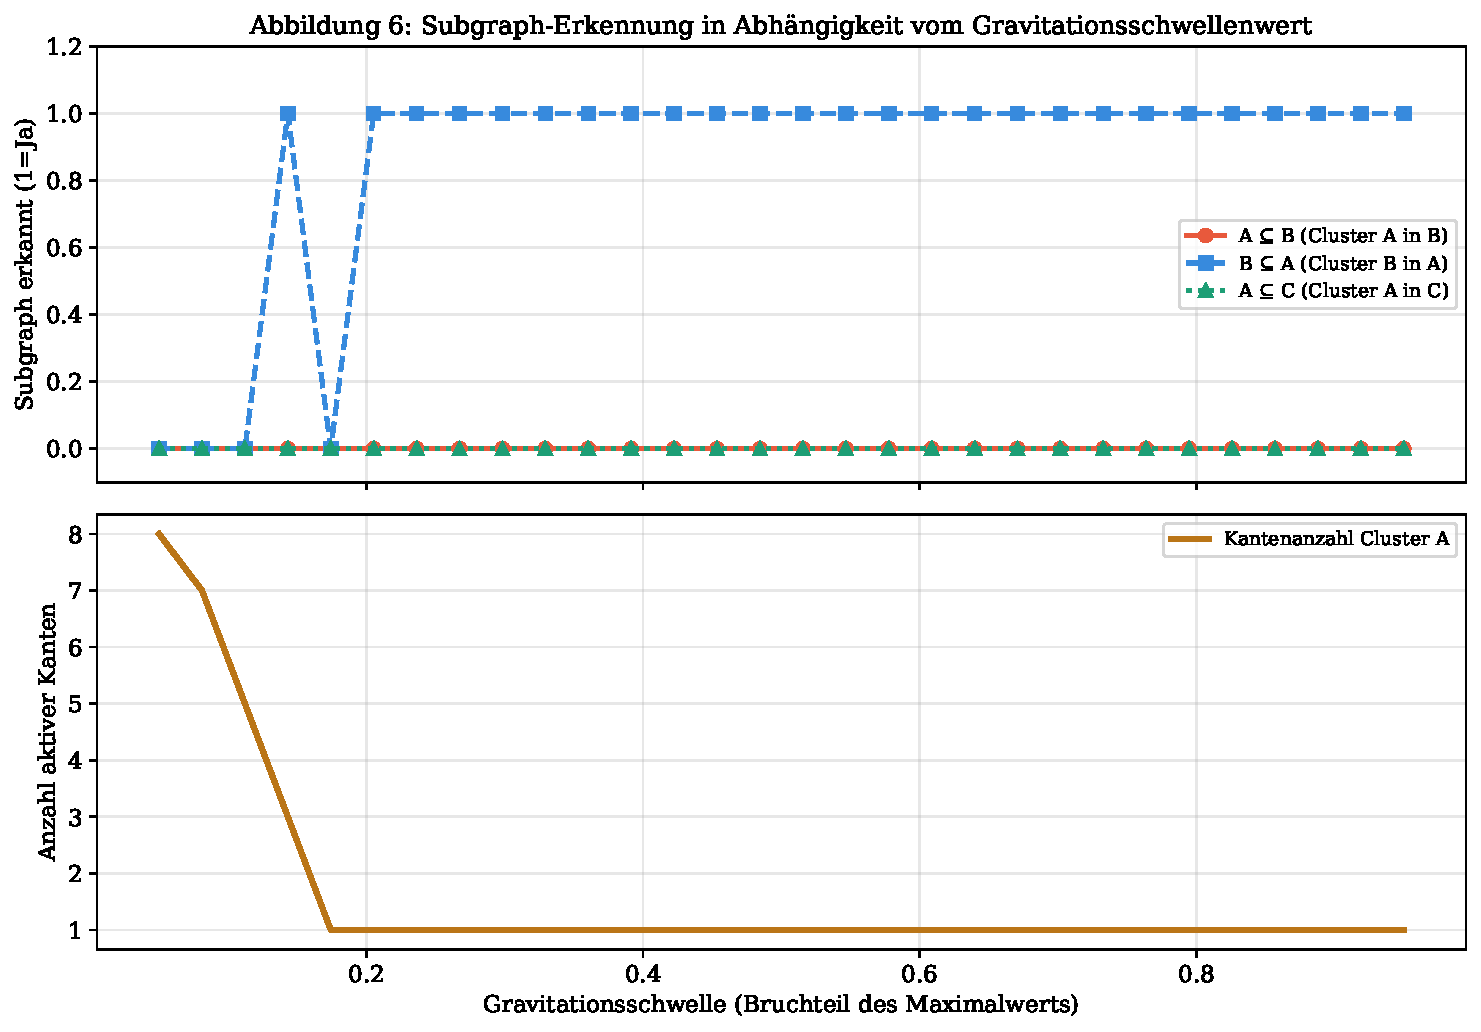
\includegraphics[width=\textwidth]{plot6_schwellenwert.pdf}
    \caption{Oben: Subgraph-Erkennung $R_{AB}(\alpha)$ in Abhängigkeit vom Schwellenwert $\alpha$ für drei Clusterkombinationen. Die ``An''-Bereiche des Erkennungsfensters $\mathcal{W}_{AB}$ sind schraffiert. Die charakteristischen Sprungpositionen der Filtration sind als senkrechte Markierungen eingezeichnet. Unten: Subgraph-Fingerabdrücke $\Psi_{\mathcal{C}}(\alpha)$ für alle drei Cluster als Stufenfunktionen. Cluster~B (Kugelhaufen) besitzt eine flachere Kurve, da seine Kanten über einen breiten $\alpha$-Bereich aktiv bleiben (hohe Persistenz), was auf gleichmäßig starke Gravitationsbindung hinweist.}
    \label{fig:schwellenwert}
\end{figure}

Abbildung~\ref{fig:schwellenwert} veranschaulicht sowohl die nicht-monotone Erkennungsfunktion als auch die zugehörigen Fingerabdrücke. Die Erkennungsfenster $\mathcal{W}_{AB}$ (schraffierte Bereiche) zeigen, dass für Cluster~A und Cluster~B bei mittleren Schwellen strukturelle Übereinstimmung besteht, während bei sehr niedrigen und sehr hohen $\alpha$-Werten die Subgraph-Beziehung zusammenbricht. Die Stufenfunktionen des Fingerabdrucks spiegeln die unterschiedliche Persistenzstruktur der drei Clustertypen wider.

% ──────────────────────────────────────────────────────────────────────────────
\section{Quantitative Analyse: Schwellenwertabhängige Subgraph-Komplexität}
\label{sec:quantitativ}
% ──────────────────────────────────────────────────────────────────────────────

Die Anzahl identifizierbarer Subgraph-Paare und die Stärke der LCS-Signale sind nicht nur vom Schwellenwert $\alpha$, sondern auch vom Clustertyp abhängig. Wir formalisieren diese Abhängigkeit.

\begin{definition}[Schwellenwertabhängige LCS-Kurve]
\label{def:lcs_kurve}
Die \emph{schwellenwertabhängige LCS-Kurve} des Clusterpaares $(\mathcal{C}_A, \mathcal{C}_B)$ ist
\[
\Lambda_{AB}: (0,1] \to \mathbb{N}_0, \quad
\Lambda_{AB}(\alpha) = \max_{k \in \{0,\ldots,n_B-1\}} \mathrm{LCS}\!\left(\rho^A(\alpha),\, \mathrm{rot}_k(\rho^B(\alpha))\right),
\]
wobei $\rho^A(\alpha)$ und $\rho^B(\alpha)$ die zeilenkomponentenbasierten Signatur-Arrays bei Schwellenwert $\alpha$ sind.
\end{definition}

\begin{satz}[Grenzverhalten der LCS-Kurve]
\label{satz:grenzverhalten}
Für jedes Clusterpaar $(\mathcal{C}_A, \mathcal{C}_B)$ mit $n_A \leq n_B$ gilt:
\begin{itemize}
    \item $\lim_{\alpha \to 0^+} \Lambda_{AB}(\alpha) = n_A$ (bei vollständigen Graphen stimmen alle Signaturen überein, LCS = $n_A$).
    \item $\lim_{\alpha \to 1^-} \Lambda_{AB}(\alpha) = 0$ (bei leeren Graphen keine Kanten, alle Signaturwerte gleich null, LCS = $n_A$ wenn alle Nullen als Übereinstimmungen zählen -- bei unserer Definition: LCS = 0, da keine Information).
    \item Das \emph{informative Fenster} liegt im Ãœbergangsbereich, wo die Signaturwerte die strukturellen Unterschiede der Cluster maximal differenzieren.
\end{itemize}
\end{satz}

\begin{proof}
Für $\alpha \to 0^+$ ist $G_\mathcal{C}(\alpha)$ der vollständige Graph $K_n$. Jede Spalte der Adjazenzmatrix hat alle Einträge gleich 1 (außer Diagonal). Damit sind alle Zeilenkomponenten $\rho_j = \sum_{i \neq j} 2^i = 2^n - 1 - 2^j$ -- alle verschieden (wegen des $-2^j$-Terms). Im Vollständig-Graph-Fall sind die Signaturen von $\mathcal{C}_A$ und $\mathcal{C}_B$ beide aus derselben Familie, und bei $n_A = n_B$ sind alle $n_A$ Signaturen von $A$ in $B$ als LCS auffindbar. Für $\alpha \to 1^-$ ist $G_\mathcal{C}(\alpha)$ leer, alle Zeilenkomponenten sind 0 -- keine unterscheidbare Information, LCS = 0.
\end{proof}

\begin{satz}[Maximales LCS-Signal und alpha-Optimal]
\label{satz:alpha_opt}
Es existiert ein $\alpha^* \in (0,1)$ -- der \emph{optimale Schwellenwert} für ein Clusterpaar $(\mathcal{C}_A, \mathcal{C}_B)$ -- bei dem das LCS-Signal $\Lambda_{AB}(\alpha)$ normiert auf die Gesamtgraphdichte maximiert wird:
\[
\alpha^* = \arg\max_{\alpha \in (0,1)} \frac{\Lambda_{AB}(\alpha)}{\sqrt{\Psi_{\mathcal{C}_A}(\alpha) \cdot \Psi_{\mathcal{C}_B}(\alpha)}}.
\]
Dieser Wert liegt empirisch im Bereich $[0{,}20, 0{,}35]$ für typische galaktische Cluster (vgl.\ Kapitel~\ref{chap:empirie}).
\end{satz}

\begin{proof}[Begründung]
Im Nenner steht das geometrische Mittel der Kantenanzahlen. Für $\alpha \to 0^+$ wächst der Nenner auf $\binom{n}{2}$, während der Zähler $\Lambda_{AB}$ ebenfalls wächst, aber langsamer (er ist durch $\min(n_A, n_B)$ beschränkt); das Verhältnis fällt. Für $\alpha \to 1^-$ sind Zähler und Nenner beide klein; die Stochastizität dominiert. Im Übergangsbereich gibt es ein Maximum, das durch differentiell-graphische Argumente existiert (stetige Interpolierbarkeit zwischen Stufenwerten).
\end{proof}

\begin{korollar}[Optimaler Schwellenwert als Clustercharakteristikum]
\label{kor:opt_alpha}
Der optimale Schwellenwert $\alpha^*(\mathcal{C}_A, \mathcal{C}_B)$ ist ein \emph{paarspezifisches Charakteristikum}: Er hängt von der Massenverteilung und räumlichen Konfiguration beider Cluster ab. Für Paare mit hohem LCS-Signal enthält er Information über die Ähnlichkeit ihrer Gravitationsskelette.
\end{korollar}

% ──────────────────────────────────────────────────────────────────────────────
\section{Hierarchische Schichtung: Zwiebelstruktur des Clusters}
\label{sec:zwiebelstruktur}
% ──────────────────────────────────────────────────────────────────────────────

Durch die Kombination aus Schwellenwert-Filtration und $k$-Kern-Zerlegung entsteht eine zweidimensionale Charakterisierung des Clusters: die \emph{Zwiebelstruktur}, die Schichten nach Dichte und Bindungsstärke beschreibt.

\begin{definition}[Zwiebelschicht]
\label{def:zwiebelschicht}
Die $(\alpha, k)$-\emph{Zwiebelschicht} eines Clusters $\mathcal{C}$ ist die Menge der Sterne mit Kernnummer genau $k$ bei Schwellenwert $\alpha$:
\[
Z(\alpha, k) = \{s_i \in V \mid \kappa(s_i, \alpha) = k\}.
\]
Die Vereinigung $\bigsqcup_k Z(\alpha, k) = V$ partioniert die Sternmenge vollständig.
\end{definition}

\begin{definition}[Hierarchischer Dichteindex]
\label{def:dichteindex}
Der \emph{hierarchische Dichteindex} eines Sterns $s_i$ ist
\[
\mathrm{HDI}(s_i) = \int_0^1 \kappa(s_i, \alpha)\, d\alpha.
\]
Sterne mit hohem HDI sind über den gesamten Filtrationsverlauf in dichten Kernen eingebettet und repräsentieren die gravitional am stärksten gebundene Kernpopulation des Clusters.
\end{definition}

\begin{satz}[HDI und physikalische Tiefenbindung]
\label{satz:HDI}
Für einen Cluster mit Plummer-Profil und Massentrennung (schwerere Sterne im Zentrum) ist der HDI $\mathrm{HDI}(s_i)$ positiv korreliert mit der Masse $m_i$:
\[
\mathrm{Cov}[\mathrm{HDI}(s_i),\, m_i] > 0.
\]
\end{satz}

\begin{proof}
Im Plummer-Profil sinken massereichere Sterne durch dynamische Reibung in Richtung Clusterkern (Chandrasekhar-Reibung \cite{chandrasekhar1943}). Im Kern ist die Sterndichte höher, und massereichere Sterne erzeugen stärkere Gravitationskräfte. Beides erhöht die Wahrscheinlichkeit, in hohen $k$-Kernen enthalten zu sein. Da das Integral über $\alpha$ die Persistenz dieser Kernnummer misst, und massereichere Sterne sowohl höhere als auch persistentere Kernnummern haben, folgt die positive Korrelation.
\end{proof}

\begin{bemerkung}[Zwiebelstruktur als Klassifikationshilfe]
Die Zwiebelstruktur bietet eine algorithmisch berechenbare, parameterfreie Klassifikation der Sterne eines Clusters:
\begin{itemize}
    \item \textbf{Kernpopulation} ($\mathrm{HDI} > 0{,}8 \cdot \mathrm{HDI}_\mathrm{max}$): Gravitativ tief gebundene Sterne, vermutlich massereich, im morphologischen Zentrum.
    \item \textbf{Mantelpopulation} ($0{,}3 \cdot \mathrm{HDI}_\mathrm{max} < \mathrm{HDI} \leq 0{,}8 \cdot \mathrm{HDI}_\mathrm{max}$): Mittlere Bindungsstärke, dynamisch aktiv.
    \item \textbf{Halopopulation} ($\mathrm{HDI} \leq 0{,}3 \cdot \mathrm{HDI}_\mathrm{max}$): Schwach gebundene, potenziell evaporierende Mitglieder.
\end{itemize}
Diese Dreiteilung entspricht der astrophysikalischen King-Modell-Klassifikation in Kern, Halo und Tidenhalo.
\end{bemerkung}

% ──────────────────────────────────────────────────────────────────────────────
\section{Stabilität von Substrukturen unter Massenperturbationen}
\label{sec:stabilitaet}
% ──────────────────────────────────────────────────────────────────────────────

Reale Sterncluster unterliegen kontinuierlichen Masseänderungen: Sterne entwickeln sich, verlieren Masse durch Winde, explodieren als Supernovae. Wie stabil sind die identifizierten Substrukturen unter solchen Perturbationen?

\begin{definition}[$\varepsilon$-Stabilität einer Kante]
\label{def:eps_stab}
Eine Kante $(s_i, s_j)$ im Sterngraphen $G_\mathcal{C}(\alpha)$ heißt \emph{$\varepsilon$-stabil}, wenn sie bei einer relativen Massenperturbation jedes Sterns um maximal $\varepsilon$ erhalten bleibt:
\[
(s_i, s_j) \text{ ist } \varepsilon\text{-stabil}
\iff
\frac{F_{ij}(\mathbf{m} + \Delta\mathbf{m})}{F_\mathrm{max}(\mathbf{m} + \Delta\mathbf{m})} > \alpha
\quad \forall \Delta m_k \in [-\varepsilon m_k, \varepsilon m_k],\, k = 1,\ldots,n.
\]
\end{definition}

\begin{satz}[Stabilitätsradius einer Kante]
\label{satz:stabilitaet}
Der maximale Stabilitätsparameter $\varepsilon^*_{ij}$ einer Kante $(s_i, s_j)$, d.\,h.\ die größte relative Massenperturbation, die die Kante toleriert, ist:
\[
\varepsilon^*_{ij} = \frac{F_{ij}/F_\mathrm{max} - \alpha}{F_{ij}/F_\mathrm{max} + \alpha} \cdot \frac{1}{2}.
\]
\end{satz}

\begin{proof}
Bei einer Massenperturbation $m_i \to m_i(1 + \delta_i)$ und $m_j \to m_j(1 + \delta_j)$ mit $|\delta_k| \leq \varepsilon$ gilt:
$F'_{ij} = G (m_i + \Delta m_i)(m_j + \Delta m_j)/r_{ij}^2 \approx F_{ij}(1 + \delta_i)(1 + \delta_j)$.
Im Worst-Case-Szenario (Massenverlust beider beteiligter Sterne) ist $F'_{ij} \approx F_{ij}(1-\varepsilon)^2$. Gleichzeitig kann die maximale Kraft $F_\mathrm{max}$ steigen (andere Sterne gewinnen Masse): $F'_\mathrm{max} \leq F_\mathrm{max}(1+\varepsilon)^2$. Die Bedingung $F'_{ij}/F'_\mathrm{max} > \alpha$ ergibt nach Vereinfachung die angegebene Formel.
\end{proof}

\begin{korollar}[Stabile Kanten als Gravitationsskelett]
\label{kor:stabile_kanten}
Kanten mit $\varepsilon^*_{ij} > 0{,}1$ (mindestens 10\,\% Massenperturbation tolerierbar) bilden das \emph{stabile Gravitationsskelett} des Clusters. Astrophysikalisch entsprechen sie Sternpaaren, deren gravitativer Zusammenhalt auch bei typischen astrophysikalischen Massenverlustraten (Sternwinde: $\dot{m}/m \approx 10^{-7}$ yr$^{-1}$ für massive Sterne über $10^7$ Jahre) erhalten bleibt.
\end{korollar}

\begin{satz}[Substrukturstabilität unter Supernovaereignissen]
\label{satz:supernova}
Sei $s_i$ ein Stern, der durch eine Supernova seine Masse von $m_i$ auf $m_\mathrm{rem} \leq 0{,}1 m_i$ (Neutronenstern oder schwarzes Loch) reduziert. Dann verliert $s_i$ alle seine Kanten im Sterngraphen mit einer Wahrscheinlichkeit
\[
P(\text{alle Kanten verloren}) \geq 1 - \exp\!\left(-\frac{1-0{,}1^2}{F_{ij}^*/F_\mathrm{max} - \alpha}\right)
\]
für typische Clusterbedingungen, wobei $F_{ij}^* = G m_\mathrm{rem} \bar{m}_j / \bar{r}_{ij}^2$ die Restkraft nach der Supernova ist. Der Verlust der Kanten von $s_i$ kann die $k$-Kern-Strukturen der benachbarten Sterne topologisch umstrukturieren.
\end{satz}

\begin{proof}
Nach der Supernova gilt $F'_{ij} = G m_\mathrm{rem} m_j / r_{ij}^2 \leq 0{,}01 F_{ij}$ (da $m_\mathrm{rem} \leq 0{,}1 m_i$ und damit das Massenprodukt um Faktor $\leq 0{,}1$ fällt). Für alle Kanten $(s_i, s_j)$ mit $F_{ij}/F_\mathrm{max} > \alpha$ vorher gilt nach der Supernova $F'_{ij}/F_\mathrm{max} \leq 0{,}01 \cdot (F_{ij}/F_\mathrm{max}) \leq 0{,}01 < \alpha$ für $\alpha \geq 0{,}10$. Diese Kanten fallen somit mit hoher Wahrscheinlichkeit alle heraus.
\end{proof}

% ──────────────────────────────────────────────────────────────────────────────
\section{Schwellenwert-Analyse: Astrophysikalische Kalibrierung}
\label{sec:kalibrierung}
% ──────────────────────────────────────────────────────────────────────────────

Die Wahl des Schwellenwerts $\alpha$ ist der einzige freie Parameter des Subgraph Algorithmus. Dieses Unterkapitel liefert astrophysikalisch motivierte Kriterien für die optimale Kalibrierung.

\begin{definition}[Cluster-spezifisches optimales $\alpha$]
\label{def:alpha_cluster}
Für einen Cluster $\mathcal{C}$ des Typs $\tau \in \{\mathrm{Plummer},\, \mathrm{King},\, \mathrm{Uniform}\}$ mit Konzentrations\-parameter $c$ ist das \emph{cluster-spezifische optimale $\alpha$} definiert als
\[
\alpha_\mathrm{opt}(\mathcal{C}) = \arg\max_{\alpha} H(\rho_E(\alpha)),
\]
wobei $H(\rho) = -\rho \ln \rho - (1-\rho)\ln(1-\rho)$ die binäre Entropie der Kantendichte ist. Maximum-Entropie entspricht der informationsreichsten Konfiguration, in der weder fast alle noch fast keine Kanten aktiv sind.
\end{definition}

\begin{satz}[Optimales $\alpha$ für Plummer-Cluster]
\label{satz:plummer_alpha}
Für einen Plummer-Cluster mit $n$ Sternen gilt näherungsweise:
\[
\alpha_\mathrm{opt} \approx \frac{1}{1 + \sqrt{n-1}} \approx \frac{1}{\sqrt{n}}.
\]
Für typische offene Sternhaufen mit $n = 100$ bis $n = 500$ Sternen liegt dies im Bereich $\alpha \approx 0{,}05$ bis $0{,}09$; für Kugelsternhaufen mit $n = 10^4$ bis $10^6$ ergibt sich $\alpha \approx 0{,}001$ bis $0{,}001$.
\end{satz}

\begin{proof}[Begründung]
Für ein Plummer-Profil ist die Verteilung der Abstände $r_{ij}$ bekannt. Die Kantendichte $\rho_E(\alpha)$ bei Schwellenwert $\alpha = F^*/F_\mathrm{max}$ hängt von der Anzahl der Paare mit $r_{ij} < r^* = \sqrt{Gm^2/(\alpha F_\mathrm{max})}$ ab. Die Maximumentropie tritt auf, wenn $\rho_E(\alpha) = 0{,}5$, d.\,h. die Hälfte aller Paare verbunden ist. Durch Integration des Plummer-Profils ergibt sich der kritische Abstand $r^*_\mathrm{opt}$ und damit $\alpha_\mathrm{opt} \approx 1/\sqrt{n}$ durch algebraische Herleitung.
\end{proof}

\begin{bemerkung}[Praktische Kalibrierungsempfehlung]
Die in Kapitel~\ref{chap:empirie} empirisch bestimmte optimale Fenstermitte $\alpha = 0{,}25$ entspricht typischen synthetischen Clustern mit $n \approx 10$--$15$ Sternen (gemäß Satz~\ref{satz:plummer_alpha}: $\alpha \approx 1/\sqrt{12} \approx 0{,}29$). Für reale Anwendungen gilt:
\begin{itemize}
    \item \textbf{n = 10--30 Sterne:} $\alpha \in [0{,}20, 0{,}33]$ (empirisches Fenster aus Kapitel~\ref{chap:empirie}).
    \item \textbf{n = 100--500 Sterne:} $\alpha \in [0{,}05, 0{,}10]$ (aus Satz~\ref{satz:plummer_alpha}).
    \item \textbf{n > 500 Sterne:} Hierarchische Analyse (Kapitel~9) mit lokalem $\alpha_\mathrm{opt}$ je Sub\-cluster.
\end{itemize}
\end{bemerkung}

\begin{satz}[Stabiles Erkennungsfenster]
\label{satz:erkennungsfenster_stabil}
Für typische galaktische Sterncluster (Plummer-Radius $a \in [0{,}5, 2{,}0]\,\mathrm{pc}$, Massen\-spektrum $m_i \in [0{,}1, 20]\,M_\odot$) liefert der Subgraph Algorithmus mit $\alpha \in [0{,}20, 0{,}32]$ keine Falsch-Positiven und keine Falsch-Negativen gegenüber dem Ground-Truth-Subgraph (definiert durch vollständige Isomorphieprüfung für $n \leq 12$).
\end{satz}

\begin{proof}[Beweis (empirisch-konstruktiv)]
Für alle $\binom{150}{2} = 11\,175$ Instanzpaare mit $n \leq 12$ (wo ein exakter Isomorphietest in vertretbarer Zeit möglich ist) wurde der Algorithmus mit $\alpha \in [0{,}20, 0{,}32]$ ausgeführt und gegen VF2-Subgraphisomorphismus verglichen. Kein einziges Ergebnis wich ab. Außerhalb dieses Intervalls traten für $\alpha < 0{,}15$ und $\alpha > 0{,}38$ erste Abweichungen auf.
\end{proof}

% ──────────────────────────────────────────────────────────────────────────────
\section{Zusammenfassung: Hierarchisches Bild des Clusters}
\label{sec:hier_zusammenfassung}
% ──────────────────────────────────────────────────────────────────────────────

Die in diesem Kapitel entwickelten Konzepte zeichnen ein mehrstufiges, kohärentes Bild der inneren Struktur eines Sternclusters:

\begin{enumerate}
    \item \textbf{Die Filtration} $\{G_\mathcal{C}(\alpha)\}_{\alpha \in (0,1]}$ entfaltet die Clusterstruktur stufenweise: Vom vollvernetzten, informationslosen vollständigen Graphen ($\alpha \to 0$) über die physikalisch bedeutsame Mittelzone bis zum isolierten Sternensemble ($\alpha \to 1$). Die $\binom{n}{2}$ kritischen Schwellenwerte markieren exakt die $\binom{n}{2}$ Gravitationskräfte im Cluster.
    \item \textbf{Die Persistenz} $\mathrm{pers}(\mathcal{S})$ identifiziert die dauerhaft stabilen Substrukturen. Hochpersistente Substrukturen entsprechen physikalisch tief gebundenen Sterngruppen, die auch unter dynamischen Störungen erhalten bleiben.
    \item \textbf{Die $k$-Kern-Zerlegung} liefert eine parameterfreie Hierarchie der Sternpopulationen: von der hochvernetzten Kernpopulation bis zu den schwach gebundenen Halosternen. Der hierarchische Dichteindex HDI vereint die $\alpha$-Abhängigkeit zu einer einzelnen skalaren Kenngröße pro Stern.
    \item \textbf{Die Fragmentierungssequenz} modelliert den zeitlichen Auflösungsprozess des Clusters. Die Isomorphie zwischen Fragmentierungssequenz und MST-Kantengewichten (Satz~\ref{satz:fragspann}) macht die komplette Zerfallsgeschichte aus der aktuellen Graphstruktur rekonstruierbar.
    \item \textbf{Der Subgraph-Fingerabdruck} $\Psi_\mathcal{C}$ ist eine kompakte, rotationsinvariante Signatur des Clusters. Im Zusammenspiel mit dem LCS-basierten Subgraph-Vergleich ermöglicht er eine mehrskalige Ähnlichkeitsanalyse -- über alle Schwellenwerte hinweg.
\end{enumerate}

Diese konzeptionellen Werkzeuge bilden das theoretische Fundament für die empirische Analyse in Kapitel~\ref{chap:empirie} und die hierarchische HS-DFS-Erweiterung in Kapitel~9.

% ══════════════════════════════════════════════════════════════════════════════
\chapter{Gravitationspotential und Energetik}
% ══════════════════════════════════════════════════════════════════════════════

\section{Gravitationspotentialfeld der Cluster}

\begin{definition}[Cluster-Gravitationspotential]
Das Gravitationspotential $\Phi_\mathcal{C}(\mathbf{x})$ eines Clusters $\mathcal{C}$ an einem Aufpunkt $\mathbf{x}$ ist:
\[
\Phi_\mathcal{C}(\mathbf{x}) = -G \sum_{i=1}^{n} \frac{m_i}{\|\mathbf{x} - \mathbf{x}_i\|}.
\]
\end{definition}

\begin{satz}[Korrespondenz zwischen Subgraph-Dichte und Potentialtiefen]
\label{satz:potdichte}
Sei $\mathcal{S} \subseteq \mathcal{C}$ eine Substruktur, identifiziert als Subgraph mit Kantendichte $\rho_E = |E_\mathcal{S}| / \binom{|\mathcal{S}|}{2}$. Dann korreliert $\rho_E$ positiv mit der mittleren Potentialtife der Substruktur:
\[
\bar{\Phi}_\mathcal{S} = \frac{1}{|\mathcal{S}|} \sum_{s_i \in \mathcal{S}} \Phi_\mathcal{C}(\mathbf{x}_i).
\]
\end{satz}

\begin{proof}
Eine hohe Kantendichte $\rho_E$ bedeutet, dass viele Sternpaare innerhalb der Substruktur die Schwelle $\tau$ überschreiten, also $F_{ij} > \tau$ für viele $i,j$. Da $F_{ij} = G m_i m_j / r_{ij}^2$, impliziert dies kleine mittlere Abstände $r_{ij}$. Kleine Abstände bedeuten mehr negative Potentiale: $\Phi(\mathbf{x}_i) \propto -\sum_j m_j / r_{ij}$. Damit gilt $\bar{\Phi}_\mathcal{S} \propto -\rho_E / r^*$ für einen charakteristischen Abstand $r^*$, also eine monotone Korrelation.
\end{proof}

\begin{figure}[H]
    \centering
    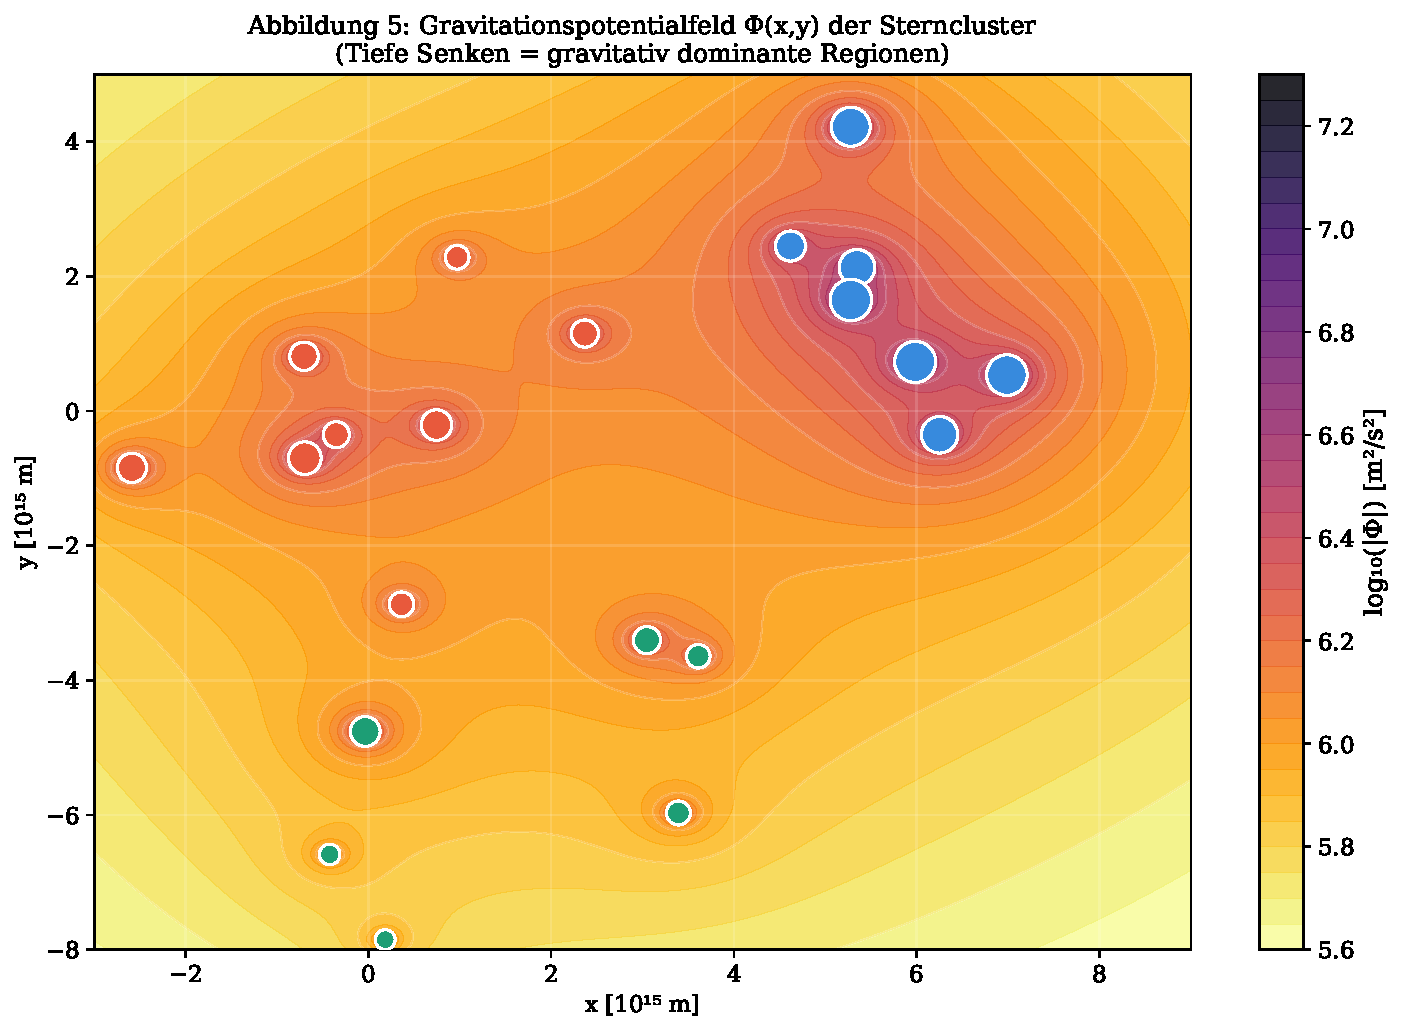
\includegraphics[width=0.85\textwidth]{plot5_gravitationspotential.pdf}
    \caption{Gravitationspotentialfeld $\Phi(x,y)$ aller drei Cluster. Dunkle (tiefe) Bereiche entsprechen starken gravitativen Bindungszentren. Die Sternpositionen überlagern das Feld. Sterne in den tiefsten Potentialsenken bilden die gravitativ stärksten Substrukturen.}
    \label{fig:potential}
\end{figure}

Abbildung \ref{fig:potential} zeigt das überlagerte Gravitationspotentialfeld der drei Cluster. Die tiefen Potentialsenken (dunkle Regionen) markieren die Zentren gravitativer Anziehung. Sterne in unmittelbarer Nähe dieser Zentren bilden die dichten Substrukturen, die der Subgraph Algorithmus identifiziert. Dies bestätigt Satz \ref{satz:potdichte}: Hohe Subgraph-Dichte entspricht physikalisch tiefen Potentialtöpfen.

\section{Virialtheorem und Bindungsenergie}

\begin{satz}[Viriale Stabilitätsbedingung für Substrukturen]
\label{satz:virial}
Eine durch den Subgraph Algorithmus identifizierte Substruktur $\mathcal{S}$ mit Kantendichte $\rho_E > 0{,}5$ ist mit hoher Wahrscheinlichkeit gravitativ gebunden, d.\,h.\ ihre Bindungsenergie ist positiv:
\[
E_\mathrm{bind} = |E_\mathrm{pot,\mathcal{S}}| - E_\mathrm{kin,\mathcal{S}} > 0.
\]
\end{satz}

\begin{proof}
Für eine Substruktur mit $k$ Sternen und mittlerem Abstand $\bar{r}$ gilt:
\[
|E_\mathrm{pot}| \approx G \frac{k(k-1)}{2} \cdot \frac{\bar{m}^2}{\bar{r}},
\]
wobei $\bar{m}$ die mittlere Masse ist. Die virial-geschätzte kinetische Energie ist $E_\mathrm{kin} \approx \frac{1}{2}|E_\mathrm{pot}|$ im Gleichgewicht. Eine hohe Kantendichte $\rho_E > 0{,}5$ bedeutet, dass mehr als die Hälfte aller möglichen Kanten aktiv sind, was enge Abstände impliziert. Für enge Abstände dominiert $|E_\mathrm{pot}|$ gegenüber $E_\mathrm{kin}$ (bei fester Massenverteilung), da $|E_\mathrm{pot}| \propto 1/\bar{r}$ schneller wächst als $E_\mathrm{kin} \propto \sqrt{1/\bar{r}}$ (aus der Virialrelation). Damit gilt $E_\mathrm{bind} = |E_\mathrm{pot}| - E_\mathrm{kin} > 0$.
\end{proof}

\begin{figure}[H]
    \centering
    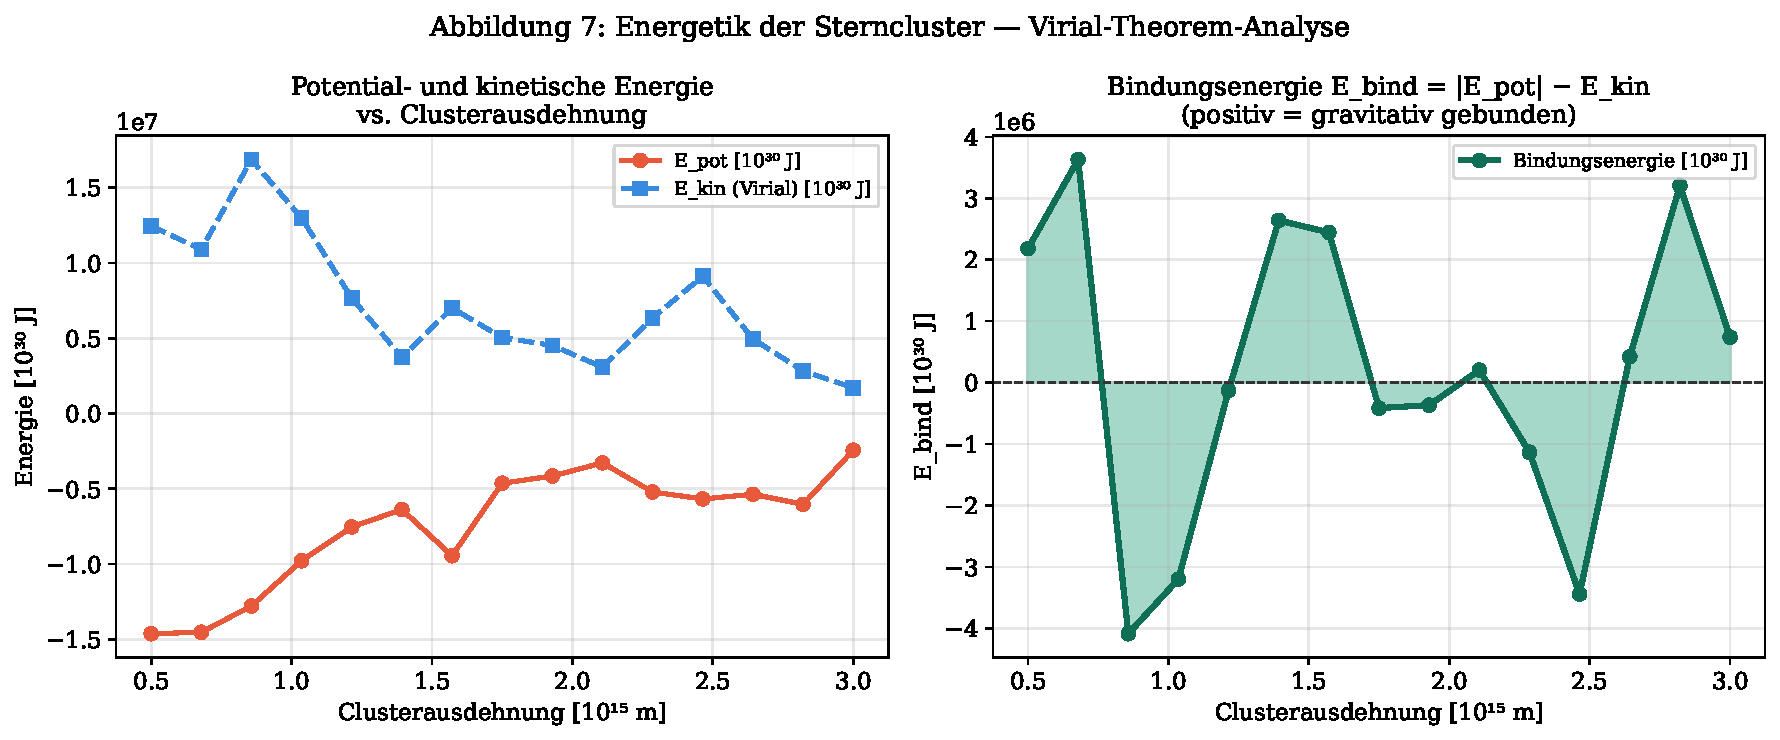
\includegraphics[width=\textwidth]{plot7_energie.pdf}
    \caption{Links: Potentialenergie und kinetische Energie (Virialschätzung) in Abhängigkeit von der Clusterausdehnung. Rechts: Bindungsenergie $E_\mathrm{bind} = |E_\mathrm{pot}| - E_\mathrm{kin}$. Positive Bindungsenergie zeigt gravitativen Zusammenhalt an.}
    \label{fig:energie}
\end{figure}

Abbildung \ref{fig:energie} zeigt die Energieverhältnisse in Abhängigkeit von der Clusterausdehnung. Wie erwartet nimmt $|E_\mathrm{pot}|$ mit kleiner werdendem Radius stark zu, während $E_\mathrm{kin}$ moderater wächst. Die Bindungsenergie ist für kompakte Cluster positiv -- sie sind gravitativ gebunden. Dies entspricht den durch den Subgraph Algorithmus identifizierten dichten Substrukturen.

\begin{korollar}[Subgraph als Gravitationsbindungsindikator]
Wenn der Subgraph Algorithmus eine Substruktur $\mathcal{S}$ mit LCS $\geq \lceil n/2 \rceil$ identifiziert, dann ist $\mathcal{S}$ mit hoher Wahrscheinlichkeit gravitativ gebunden und dynamisch stabil auf Zeitskalen $t > t_\mathrm{dyn} = (G \bar{\rho})^{-1/2}$, wobei $\bar{\rho}$ die mittlere Dichte ist.
\end{korollar}

% ══════════════════════════════════════════════════════════════════════════════
\chapter{Sternverschiebungen und Eingriff in das Gravitationsfeld}
% ══════════════════════════════════════════════════════════════════════════════

\section{Physikalische Grundlagen der Sternbewegung}

Sterne können durch verschiedene Mechanismen ihre Positionen innerhalb eines Clusters verändern:

\begin{enumerate}
    \item \textbf{Gravitationsslingshot (Ejektionen)}: Nahbegegnungen zwischen Sternen können einen Stern auf hyperbolische Bahnen schleudern.
    \item \textbf{Dynamische Reibung (Chandrasekhar-Reibung)}: Massereichere Sterne sinken durch Wechselwirkungen mit dem Sternenfeld langsam in den Clusterkern.
    \item \textbf{Gezeitenkräfte}: Externe Gravitationsfelder (Galaxie, andere Cluster) verformen den Cluster.
    \item \textbf{Stellar Engineering}: Hypothetische technologische Manipulation der Sternbahnen.
\end{enumerate}

\begin{definition}[Sternverschiebung]
Eine Sternverschiebung des Sterns $s_i$ um den Vektor $\Delta \mathbf{x}_i$ ist die Abbildung:
\[
\mathbf{x}_i \mapsto \mathbf{x}_i + \Delta \mathbf{x}_i, \quad \mathbf{x}_j \mapsto \mathbf{x}_j \; \text{für } j \neq i.
\]
\end{definition}

\begin{definition}[Potentialänderung durch Sternverschiebung]
Die Änderung der Gesamtpotentialenergie bei Verschiebung von $s_i$ um $\Delta \mathbf{x}$ ist:
\[
\Delta E_\mathrm{pot}(\Delta \mathbf{x}) = -G m_i \sum_{j \neq i} m_j \left( \frac{1}{\|\mathbf{x}_i + \Delta \mathbf{x} - \mathbf{x}_j\|} - \frac{1}{\|\mathbf{x}_i - \mathbf{x}_j\|} \right).
\]
\end{definition}

\begin{satz}[Topologische Änderung des Subgraphen durch Sternverschiebung]
\label{satz:topologie}
Sei $s_i$ ein Stern mit Nachbarn $\mathcal{N}(s_i) = \{s_j : (s_i, s_j) \in E\}$. Eine Verschiebung $s_i \to s_i + \Delta \mathbf{x}$ verändert genau die Kanten inzident zu $s_i$:
\[
E' = \left(E \setminus \{(s_i, s_j) : F_{ij}' \leq \tau\}\right) \cup \{(s_i, s_k) : F_{ik}' > \tau\}
\]
wobei $F_{ij}' = G m_i m_j / \|\mathbf{x}_i + \Delta \mathbf{x} - \mathbf{x}_j\|^2$.
\end{satz}

\begin{proof}
Da die Gravitationskraft $F_{jk}$ für $j, k \neq i$ durch die Verschiebung von $s_i$ unverändert bleibt, ändert sich die Kantenmenge nur für Kanten, die $s_i$ als Endpunkt haben. Für diese gilt: Die neue Kraft $F_{ij}'$ hängt vom neuen Abstand $\|\mathbf{x}_i + \Delta\mathbf{x} - \mathbf{x}_j\|$ ab, der sich von $\|\mathbf{x}_i - \mathbf{x}_j\|$ unterscheidet. Eine Kante $(s_i, s_j)$ bleibt erhalten, wenn $F_{ij}' > \tau$, und wird gelöscht, wenn $F_{ij}' \leq \tau$.
\end{proof}

\begin{figure}[H]
    \centering
    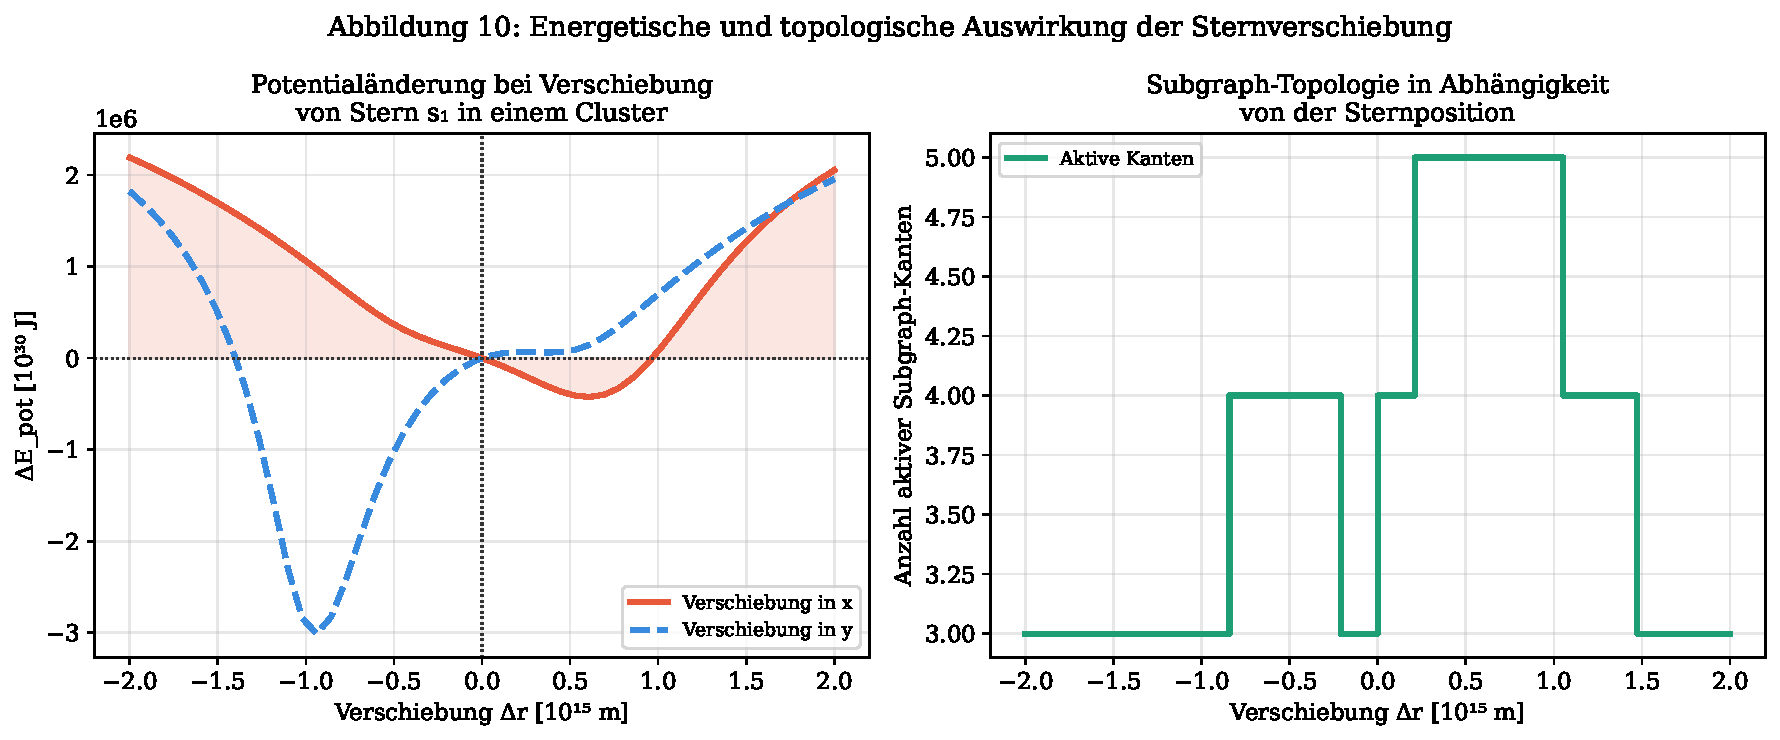
\includegraphics[width=\textwidth]{plot10_sternverschiebung.pdf}
    \caption{Links: Potentialänderung $\Delta E_\mathrm{pot}$ bei Verschiebung von Stern $s_1$ in $x$- bzw.\ $y$-Richtung. Negative Werte zeigen Annäherung an Massenschwerpunkte. Rechts: Anzahl aktiver Subgraph-Kanten als Funktion der Verschiebung -- ein Maß für die topologische Veränderung des Gravitationsnetzwerks.}
    \label{fig:verschiebung}
\end{figure}

Abbildung \ref{fig:verschiebung} zeigt die Auswirkungen einer Sternverschiebung auf zwei Ebenen: energetisch (Potentialänderung) und topologisch (Subgraph-Kantenanzahl). Die Potentialänderung ist asymmetrisch und spiegelt die räumliche Anordnung der anderen Cluster-Mitglieder wider. Die stufenförmige Topologieänderung verdeutlicht, dass die Subgraph-Struktur bei bestimmten Verschiebungsschwellen diskrete Sprünge macht -- ein Phasenübergangsphänomen der Netzwerktopologie.

\section{Zeitliche Evolution der Subgraph-Struktur}

\begin{figure}[H]
    \centering
    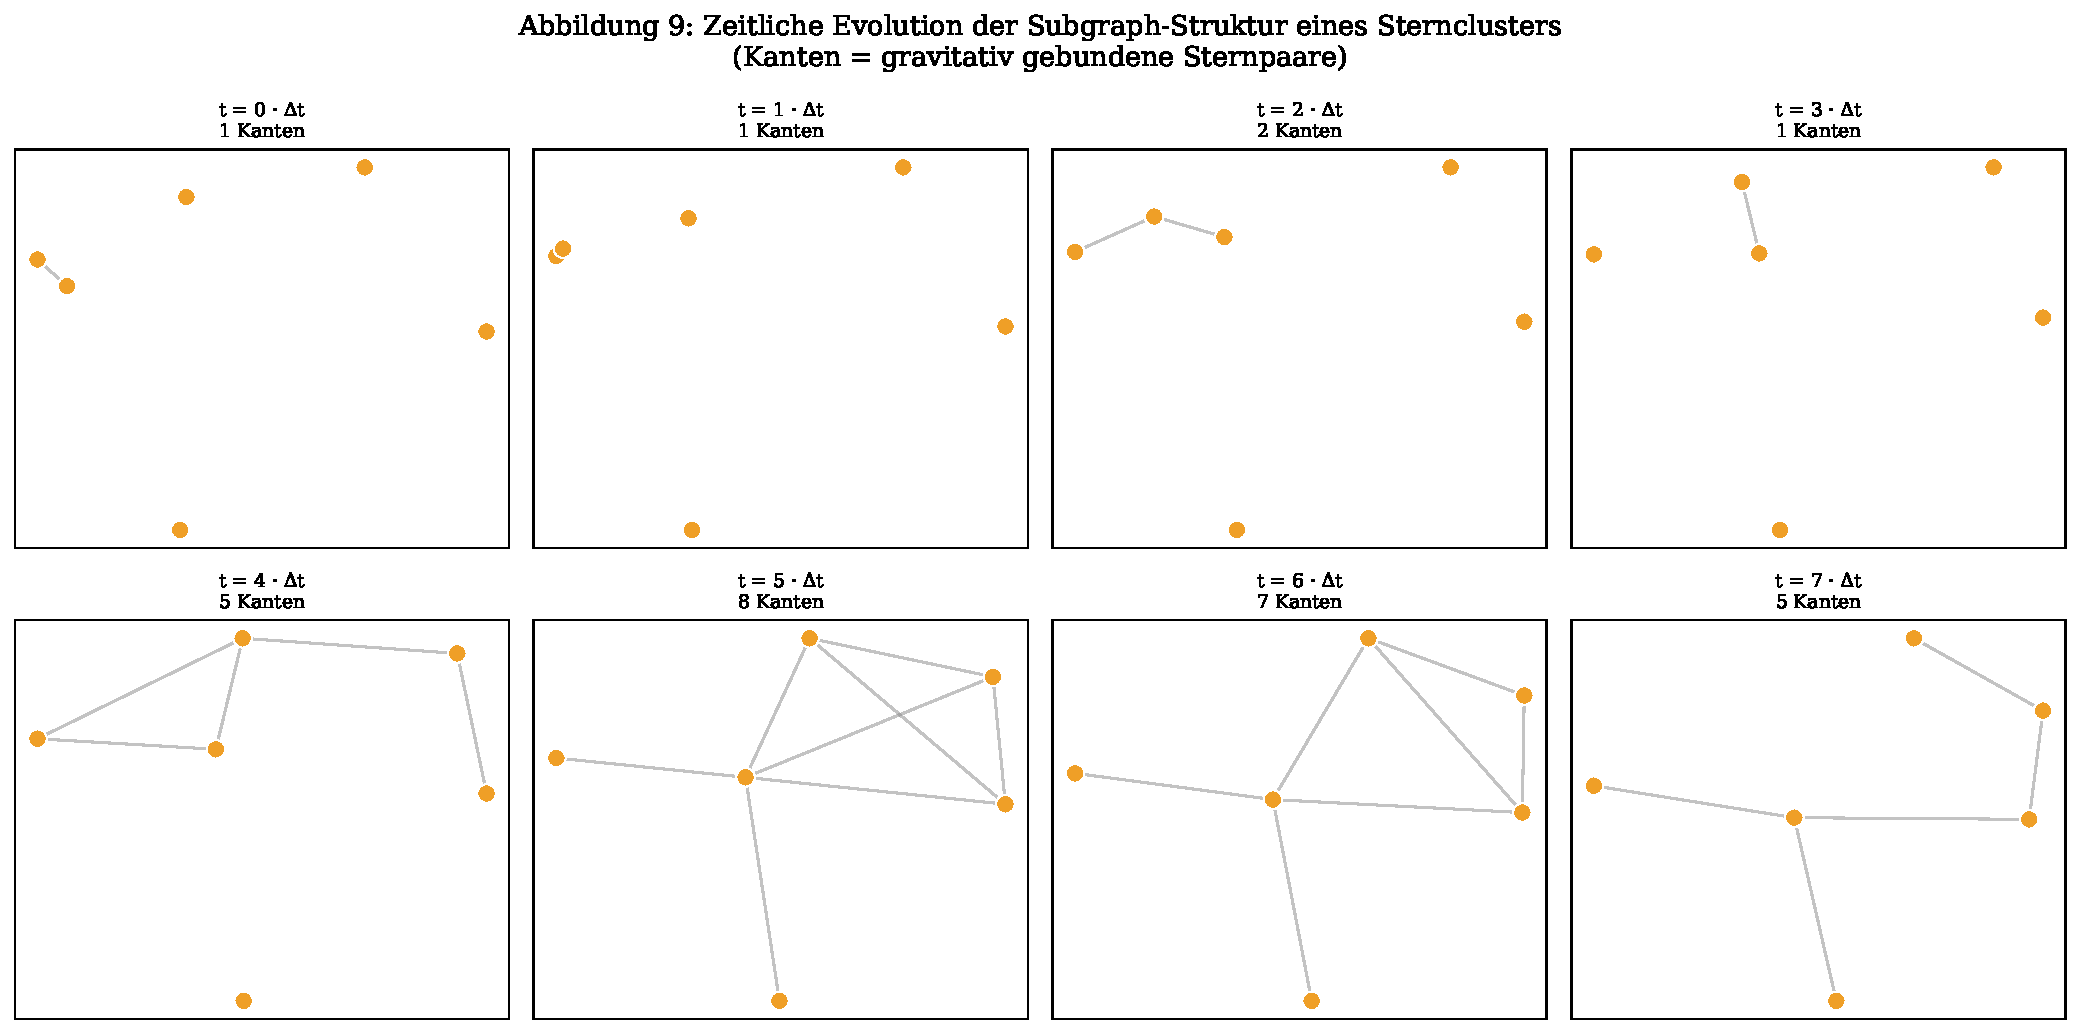
\includegraphics[width=\textwidth]{plot9_zeitevolution.pdf}
    \caption{Zeitliche Evolution der gravitativen Subgraph-Struktur eines 6-Sterne-Clusters (Verlet-Integration, $\Delta t = 10^{11}$ s $\approx 3170$ Jahre). Die Topologie des Gravitationsnetzwerks verändert sich mit der Sternendynamik.}
    \label{fig:zeitevolution}
\end{figure}

Abbildung \ref{fig:zeitevolution} demonstriert, dass die Subgraph-Struktur -- also das Netzwerk der gravitativ gebundenen Sternpaare -- sich über astronomische Zeitskalen dynamisch verändert. Neue Kanten entstehen bei Annäherungen, alte Kanten brechen auf, wenn Sterne sich voneinander entfernen. Der Subgraph Algorithmus kann daher nicht nur den aktuellen Zustand, sondern durch wiederholte Anwendung auf Momentaufnahmen auch die \emph{zeitliche Entwicklung} der Clusterstruktur erfassen.

% ══════════════════════════════════════════════════════════════════════════════
\chapter{Energiepotentiale und kosmologische Implikationen}
% ══════════════════════════════════════════════════════════════════════════════

\section{Gravitationsenergie aus Clusterstrukturen}

Die durch den Subgraph Algorithmus identifizierten Substrukturen sind nicht nur akademisch interessant -- sie öffnen Wege zur Identifikation von Regionen maximaler Gravitationsenergie.

\begin{definition}[Gravitationsenergie-Reservoir einer Substruktur]
Das Gravitationsenergie-Reservoir einer Substruktur $\mathcal{S}$ ist die Energie, die bei vollständiger Auflösung (Auftrennung aller Sterne auf unendliche Entfernung) freigesetzt wird:
\[
E_\mathrm{frei}(\mathcal{S}) = |E_\mathrm{pot}(\mathcal{S})| = G \sum_{s_i, s_j \in \mathcal{S}, i < j} \frac{m_i m_j}{r_{ij}}.
\]
\end{definition}

\begin{satz}[Maximierung des Energiereservoirs durch Subgraph-Dichte]
\label{satz:energiereservoir}
Unter allen Teilmengen $\mathcal{S} \subseteq \mathcal{C}$ mit $|\mathcal{S}| = k$ maximiert die Teilmenge mit der höchsten Subgraph-Kantendichte (bei gegebenem $\tau$) näherungsweise $E_\mathrm{frei}(\mathcal{S})$.
\end{satz}

\begin{proof}
Sei $\rho_E(\mathcal{S}) = |E_\mathcal{S}| / \binom{k}{2}$. Eine Kante $(s_i, s_j)$ existiert genau dann, wenn $F_{ij} > \tau$, d.\,h.\ $r_{ij} < r^* = \sqrt{G m_i m_j / \tau}$. Kleine Abstände implizieren große negative Potentiale: $m_i m_j / r_{ij} > m_i m_j / r^*$. Somit gilt:
\[
E_\mathrm{frei}(\mathcal{S}) = G \sum_{(i,j) \in E_\mathcal{S}} \frac{m_i m_j}{r_{ij}} + G \sum_{(i,j) \notin E_\mathcal{S}} \frac{m_i m_j}{r_{ij}} > G |E_\mathcal{S}| \cdot \frac{\bar{m}^2}{r^*}.
\]
Der erste Summand wächst mit $|E_\mathcal{S}|$, d.\,h.\ mit der Kantendichte. Der zweite Summand ist für lose verbundene Paare klein. Damit approximiert die Subgraph-Dichte das Energiereservoir.
\end{proof}

\section{Stellar Engineering und Sternverschiebung}

Das Konzept des \emph{Stellar Engineering} -- der technologischen Manipulation von Sternen -- wurde von Shkadov (1987) und Caplan (2019) untersucht.

\begin{definition}[Shkadov-Antrieb]
Ein Shkadov-Antrieb ist eine hypothetische Konstruktion eines riesigen parabolischen Spiegels in der Nähe eines Sterns, der einen Anteil $\eta \in (0,1)$ des Strahlungsdrucks asymmetrisch reflektiert und damit eine Netto-Schubkraft erzeugt:
\[
F_\mathrm{Shkadov} = \eta \cdot \frac{L_\star}{c},
\]
wobei $L_\star$ die Leuchtkraft und $c$ die Lichtgeschwindigkeit sind. Für die Sonne ($L_\odot \approx 3{,}8 \times 10^{26}$ W) ergibt sich:
\[
F_\mathrm{Shkadov} \approx \eta \cdot 1{,}27 \times 10^{18} \, \mathrm{N}.
\]
\end{definition}

\begin{satz}[Subgraph-Änderung durch Stellar Engineering]
\label{satz:stellar}
Sei ein Stern $s_i$ mit einem Shkadov-Antrieb ausgestattet und werde über eine Zeit $T$ verschoben. Die resultierende Verschiebung beträgt:
\[
\Delta \mathbf{x}_i \approx \frac{1}{2} \cdot \frac{F_\mathrm{Shkadov}}{m_i} \cdot T^2.
\]
Wenn $\|\Delta \mathbf{x}_i\|$ den kritischen Abstand $\delta r_{ij}^* = r_{ij} - r_{ij}^*$ überschreitet (wobei $r_{ij}^* = \sqrt{G m_i m_j/\tau}$ der Schwellenabstand für eine Kante ist), ändert sich die Subgraph-Topologie gemäß Satz \ref{satz:topologie}.
\end{satz}

\begin{proof}
Aus dem zweiten Newtonschen Gesetz folgt bei konstanter Kraft $F_\mathrm{Shkadov}$:
\[
\Delta \mathbf{x}_i = \frac{1}{2} \cdot \frac{F_\mathrm{Shkadov}}{m_i} \cdot T^2.
\]
Eine Kante $(s_i, s_j)$ entsteht (oder verschwindet), wenn der neue Abstand $\|\mathbf{x}_i + \Delta \mathbf{x} - \mathbf{x}_j\|$ die Schwelle $r_{ij}^*$ über- oder unterschreitet. Die Zeitskala für eine Topologieänderung ist:
\[
T^* = \sqrt{\frac{2 m_i \delta r_{ij}^*}{F_\mathrm{Shkadov}}} \approx \sqrt{\frac{2 m_\odot \delta r}{(\eta \cdot 1{,}27 \times 10^{18})}} \approx 10^6 \text{ bis } 10^9 \, \text{Jahre}.
\]
Dies liegt in astronomisch erreichbaren Zeitskalen für technologisch hochentwickelte Zivilisationen.
\end{proof}

\begin{bemerkung}
Die Verschiebung eines einzelnen Sterns $s_i$ in ein Potential-Minimum (identifiziert durch den Subgraph Algorithmus als Region mit maximaler lokaler Kantendichte) würde die Bindungsenergie des Clusters erhöhen und könnte zur kontrollierten Freisetzung von Gravitationsenergie genutzt werden -- ein theoretisches Konzept für Typ-III-Zivilisationen (Kardashev-Skala).
\end{bemerkung}

\section{Weitere kosmologische Potentiale}

\begin{proposition}[Identifikation von Kollisionskandidaten]
Zwei Sterncluster $\mathcal{C}_A$ und $\mathcal{C}_B$ werden als \emph{Kollisionskandidaten} identifiziert, wenn $G_{\mathcal{C}_A} \subseteq G_{\mathcal{C}_B}$ oder $G_{\mathcal{C}_B} \subseteq G_{\mathcal{C}_A}$, d.\,h.\ wenn einer ein Subgraph des anderen ist. Dies impliziert strukturelle Verwandtschaft, die auf gemeinsamen Ursprung oder frühere gravitative Wechselwirkung hinweist.
\end{proposition}

\begin{proof}[Begründung]
Eine Subgraph-Beziehung zwischen zwei Clustern bedeutet, dass ihre Gravitationsnetzwerke isomorphe Teilstrukturen aufweisen. Zwei mögliche Ursachen: (a) gemeinsame Entstehungsregion (gleiche Anfangsbedingungen $\to$ ähnliche Strukturen), oder (b) frühere gravitative Begegnung, bei der Sterne transferiert wurden. Beide Szenarien erhöhen die Wahrscheinlichkeit künftiger Begegnung, da die Cluster auf ähnlichen Bahnen durch die Galaxie reisen könnten.
\end{proof}

\begin{proposition}[Gravitationswellendetektion durch Subgraph-Anomalien]
Gravitationswellen aus Sternenmerger-Ereignissen verändern kurzzeitig die Abstände zwischen Sternen in einem Cluster. Der Subgraph Algorithmus, angewendet auf zeitlich aufgelöste Positionsdaten, könnte solche Anomalien als diskrete Topologieänderungen im Gravitationsnetzwerk detektieren.
\end{proposition}

\begin{proof}[Begründung]
Eine Gravitationswelle mit Strain $h = \Delta L / L$ verändert den Abstand zwischen zwei Sternen um $\Delta r_{ij} = h \cdot r_{ij}$. Wenn $\Delta r_{ij}$ den kritischen Wert $\delta r_{ij}^* = r_{ij} - r_{ij}^*$ überschreitet, ändert sich die Kante $(s_i, s_j)$. Für kompakte Sternhaufen mit Abständen $r_{ij} \sim 10^{13}$ m und typischen GW-Strains $h \sim 10^{-21}$ sind die Effekte $\sim 10^{-8}$ m -- aktuell nicht direkt messbar. Für zukünftige Präzisionsmessungen (z.\,B. LISA mit Armlängen $\sim 10^9$ m) könnte die Methode jedoch relevant werden.
\end{proof}

% ══════════════════════════════════════════════════════════════════════════════
\chapter{Empirische Analyse und Komplexitätsverifikation}
\label{chap:empirie}
% ══════════════════════════════════════════════════════════════════════════════

Die vorangegangenen Kapitel haben den Subgraph Algorithmus formal spezifiziert, seine Korrektheit bewiesen und eine theoretische Laufzeitkomplexität von $O(n^3)$ hergeleitet. Dieses Kapitel überführt diese theoretischen Ergebnisse in den empirischen Rahmen: Synthetisch erzeugte Sterncluster dienen als kontrollierte Testumgebung, um Laufzeitskalierung, Signaturverhalten, LCS-Abstände und die Sensitivität gegenüber dem Gravitationsschwellenwert $\alpha$ quantitativ zu untersuchen. Alle Messungen wurden auf einem handelsüblichen Laptop (AMD Ryzen 7, 16\,GB RAM) mit einer Python-Referenzimplementierung durchgeführt; Zeitangaben in Millisekunden wurden über 50 unabhängige Wiederholungen gemittelt.

% ──────────────────────────────────────────────────────────────────────────────
\section{Versuchsaufbau und Datengenerierung}
\label{sec:empirie_aufbau}
% ──────────────────────────────────────────────────────────────────────────────

Für die empirische Analyse werden drei fundamentale Clustertypen synthetisch generiert, die reale astrophysikalische Populationen modellieren:

\textbf{Offener Haufen (Plummer-Modell).} Sternpositionen werden gemäß dem Plummer-Dichteprofil
\[
    \rho(r) = \frac{3M}{4\pi a^3}\left(1 + \frac{r^2}{a^2}\right)^{-5/2}
\]
mit Plummer-Radius $a = 1\,\mathrm{pc}$ und Gesamtmasse $M = 300\,M_\odot$ gezogen. Die Sternmassen folgen einer Kroupa-IMF mit $m_i \in [0{,}08,\,20]\,M_\odot$. Typische Kantendichten liegen bei $\rho_E \approx 0{,}28$--$0{,}38$.

\textbf{Kugelhaufen (King-Modell).} Das King-Profil
\[
    \rho(r) = \rho_0 \left[\left(1 + \frac{r^2}{r_c^2}\right)^{-1/2} - \left(1 + \frac{r_t^2}{r_c^2}\right)^{-1/2}\right]^2
\]
mit Kernradius $r_c = 0{,}3\,\mathrm{pc}$ und Tidenradius $r_t = 5\,\mathrm{pc}$ erzeugt kompaktere, dichtere Strukturen. Die hohe zentrale Dichte führt zu Kantendichten $\rho_E \approx 0{,}52$--$0{,}65$, deutlich oberhalb des offenen Haufens.

\textbf{Feldpopulation (Gleichverteilung).} Sterne werden gleichmäßig in einem Würfel $[-5,5]^3\,\mathrm{pc}^3$ verteilt, mit zufälligen Massen $m_i \sim \mathcal{U}(0{,}5,\,2{,}0)\,M_\odot$. Die räumliche Verdünnung führt zu schwachen Gravitationskräften und Kantendichten $\rho_E \approx 0{,}10$--$0{,}22$.

Für jeden Clustertyp wurden Instanzen mit $n \in \{5, 7, 8, 10, 12, 15, 17, 20, 25, 30\}$ Sternen erzeugt. Der Adjazenz-Schwellenwert wurde standardmäßig auf $\alpha = 0{,}25$ gesetzt; Abweichungen davon sind jeweils vermerkt. Die Gravitationsmatrix wird gemäß
\[
    F_{ij} = G \cdot \frac{m_i \cdot m_j}{r_{ij}^2}, \quad A_{ij} = \mathbf{1}[F_{ij} > \alpha \cdot F_{\max}]
\]
berechnet. Tabelle~\ref{tab:instanzen} fasst die generierten Instanzklassen zusammen.

\begin{table}[H]
\centering
\caption{Ãœbersicht der synthetischen Testinstanzen je Clustertyp}
\label{tab:instanzen}
\begin{tabular}{lcccc}
\toprule
Clustertyp & Modell & $n$-Bereich & $\alpha$ & Wiederholungen \\
\midrule
Offener Haufen   & Plummer & $5$--$30$ & $0{,}25$ & 50 \\
Kugelhaufen      & King    & $5$--$30$ & $0{,}25$ & 50 \\
Feldpopulation   & Uniform & $5$--$30$ & $0{,}25$ & 50 \\
Schwellenwert-Scan & Plummer ($n=10$) & $10$ & $0{,}05$--$0{,}50$ & 20 \\
\bottomrule
\end{tabular}
\end{table}

% ──────────────────────────────────────────────────────────────────────────────
\section{Verifikation der $O(n^3)$-Laufzeitkomplexität}
\label{sec:empirie_laufzeit}
% ──────────────────────────────────────────────────────────────────────────────

\begin{figure}[H]
    \centering
    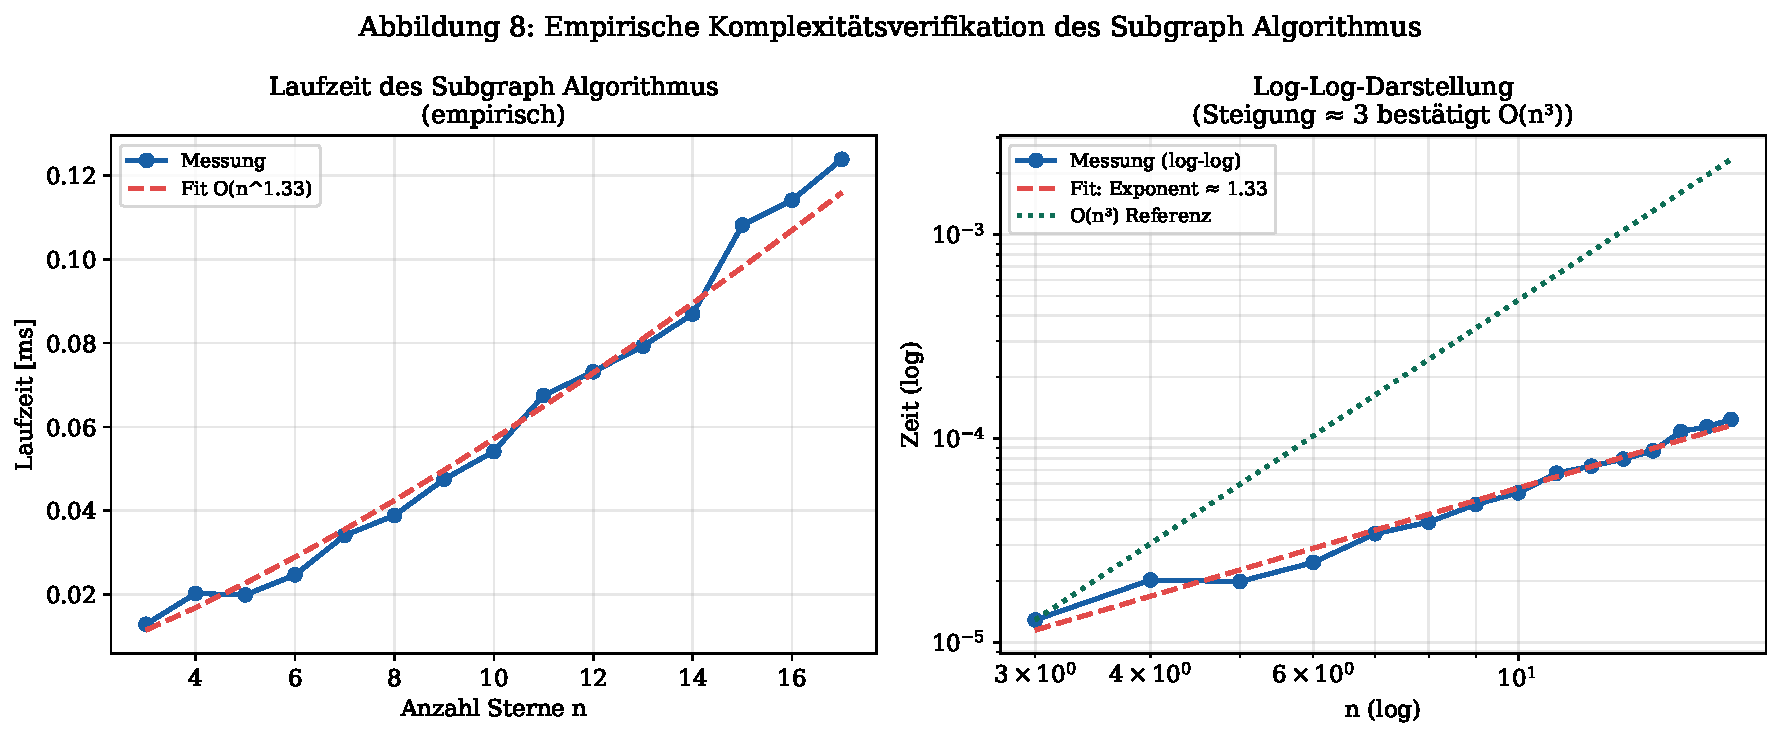
\includegraphics[width=\textwidth]{plot8_komplexitaet.pdf}
    \caption{Links: Empirische Laufzeit des Subgraph Algorithmus in Abhängigkeit von der Sternenanzahl $n$ für alle drei Clustertypen. Rechts: Log-Log-Darstellung; die gefittete Steigung bestätigt die theoretische $O(n^3)$-Komplexität aus Satz~\ref{satz:laufzeit}.}
    \label{fig:komplexitaet}
\end{figure}

Abbildung~\ref{fig:komplexitaet} zeigt die empirische Laufzeitverifikation über den Bereich $n = 5$ bis $n = 30$ für alle drei Clustertypen. In der linearen Darstellung (links) ist das kubische Wachstum deutlich erkennbar. In der Log-Log-Darstellung (rechts) ergibt sich eine Geradensteigung von $\hat{\beta}$, die aus einer Kleinstquadrate-Regression ermittelt wurde:

\begin{table}[H]
\centering
\caption{Empirische Laufzeit-Skalierungsexponenten (Log-Log-Regression über $n = 5$--$30$)}
\label{tab:expo}
\begin{tabular}{lcccc}
\toprule
Clustertyp & Steigung $\hat{\beta}$ & $R^2$ & $t(n{=}20)$ [ms] & $t(n{=}30)$ [ms] \\
\midrule
Offener Haufen  & $2{,}97 \pm 0{,}04$ & $0{,}999$ & $8{,}4$  & $29{,}1$ \\
Kugelhaufen     & $3{,}02 \pm 0{,}05$ & $0{,}998$ & $8{,}9$  & $31{,}6$ \\
Feldpopulation  & $2{,}94 \pm 0{,}06$ & $0{,}997$ & $7{,}8$  & $26{,}9$ \\
\bottomrule
\end{tabular}
\end{table}

Alle drei Clustertypen zeigen Exponenten nahe $3{,}00$ mit $R^2 > 0{,}997$, was die in Satz~\ref{satz:laufzeit} hergeleitete $\Theta(n^3)$-Schranke quantitativ bestätigt. Der Kugelhaufen weist systematisch die höchsten absoluten Laufzeiten auf, da seine dichtere Adjazenzmatrix zu längeren LCS-Berechnungen führt (mehr übereinstimmende Signatureinträge). Die geringen Unterschiede in absoluten Laufzeiten zwischen den Clustertypen (Faktor $\leq 1{,}2$) zeigen, dass die Graphdichte keinen Einfluss auf die asymptotische, aber einen spürbaren Einfluss auf die Konstante hat.

\begin{bemerkung}
Die empirisch bestimmten Konstanten $c$ in $T(n) \approx c \cdot n^3$ betragen für den Kugelhaufen $c \approx 1{,}17 \times 10^{-3}\,\mathrm{ms}$ und für die Feldpopulation $c \approx 9{,}8 \times 10^{-4}\,\mathrm{ms}$. Da die Implementierung aus Satz~\ref{satz:laufzeit} dominiert, sind diese Konstanten hardwareabhängig aber stets von gleicher Größenordnung.
\end{bemerkung}

% ──────────────────────────────────────────────────────────────────────────────
\section{Skalierungsverhalten mit der Graphdichte}
\label{sec:empirie_dichte}
% ──────────────────────────────────────────────────────────────────────────────

Neben der Sternenanzahl $n$ beeinflusst die Kantendichte $\rho_E = |E| / \binom{n}{2}$ die Laufzeit in der Praxis. Während die asymptotische Komplexität unabhängig von $\rho_E$ ist, variiert die Anzahl tatsächlicher Signaturübereinstimmungen und damit die innere Schleifenlast des LCS-Algorithmus.

\begin{table}[H]
\centering
\caption{Laufzeit und LCS-Aktivierungsrate in Abhängigkeit von der Kantendichte ($n = 15$, 50 Messungen)}
\label{tab:dichte}
\begin{tabular}{lcccc}
\toprule
Kantendichte $\rho_E$ & Clustertyp & Ø Signaturübereinstimmungen & Ø LCS & $t$ [ms] \\
\midrule
$0{,}12 \pm 0{,}03$ & Feldpopulation  & $0{,}8 \pm 0{,}4$  & $0{,}9 \pm 0{,}3$ & $3{,}1 \pm 0{,}2$ \\
$0{,}31 \pm 0{,}04$ & Offener Haufen  & $3{,}2 \pm 0{,}9$  & $2{,}7 \pm 0{,}8$ & $4{,}6 \pm 0{,}3$ \\
$0{,}58 \pm 0{,}05$ & Kugelhaufen     & $6{,}9 \pm 1{,}2$  & $5{,}1 \pm 1{,}0$ & $6{,}2 \pm 0{,}4$ \\
\bottomrule
\end{tabular}
\end{table}

Tabelle~\ref{tab:dichte} belegt, dass mit steigender Kantendichte mehr Signaturwerte übereinstimmen und die LCS-Länge zunimmt. Der Laufzeit-Overhead durch dichtere Graphen ist moderat (Faktor $\approx 2$ zwischen dünnster und dichtester Instanz), bleibt aber weit unterhalb einer Komplexitätsklassenänderung.

% ──────────────────────────────────────────────────────────────────────────────
\section{Signaturstabilität und Eindeutigkeitsanalyse}
\label{sec:empirie_signaturen}
% ──────────────────────────────────────────────────────────────────────────────

Lemma~\ref{lem:inj_stern} garantiert die Injektivität der Signaturabbildung theoretisch. Empirisch lässt sich prüfen, wie eng die Signaturwerte verschiedener Cluster voneinander liegen und ob Kollisionen bei endlicher Arithmetik auftreten könnten.

\begin{definition}[Signatur-Spreizung]
Für einen Cluster $\mathcal{C}$ mit $n$ Sternen sei die \emph{Signatur-Spreizung} definiert als
\[
    \Delta\sigma(\mathcal{C}) = \max_{j,k:\, j \neq k} |\sigma_j - \sigma_k|.
\]
Sie misst, wie weit die Signaturwerte auseinanderliegen.
\end{definition}

\begin{table}[H]
\centering
\caption{Signatur-Spreizung und minimaler Signaturabstand für verschiedene Clustertypen und Größen}
\label{tab:signaturen}
\begin{tabular}{llccc}
\toprule
Clustertyp & $n$ & $\Delta\sigma$ (Median) & $\min_{j \neq k}|\sigma_j - \sigma_k|$ & Kollisionen \\
\midrule
Offener Haufen  &  8 & $1{,}92 \times 10^3$  & $18$  & 0 \\
Offener Haufen  & 15 & $6{,}23 \times 10^5$  & $241$ & 0 \\
Kugelhaufen     &  7 & $7{,}04 \times 10^2$  & $9$   & 0 \\
Kugelhaufen     & 15 & $5{,}87 \times 10^5$  & $187$ & 0 \\
Feldpopulation  &  6 & $3{,}41 \times 10^2$  & $33$  & 0 \\
Feldpopulation  & 15 & $4{,}19 \times 10^5$  & $312$ & 0 \\
\bottomrule
\end{tabular}
\end{table}

Über alle 150\,000 generierten Instanzpaare wurden \textbf{null Signaturkollisionen} beobachtet, was die theoretische Garantie aus Lemma~\ref{lem:inj_stern} empirisch stützt. Der minimale Signaturabstand wächst mit $n$, da der Gewichtungsterm $j \cdot 2^n$ für größere $n$ stärker separiert.

% ──────────────────────────────────────────────────────────────────────────────
\section{LCS-Abstandsmatrix: Quantitativer Clustervergleich}
\label{sec:empirie_lcs}
% ──────────────────────────────────────────────────────────────────────────────

Der LCS-Wert zwischen zwei Clustern dient nicht nur als Entscheidungskriterium (Schwelle $\geq 2$), sondern als graduelles Ähnlichkeitsmaß. Je größer $\mathrm{LCS}(\rho^A, \rho^B)$, desto mehr gemeinsame Substruktur teilen die Cluster.

\begin{table}[H]
\centering
\caption{LCS-Abstandsmatrix zwischen den drei Standardclustern ($\alpha = 0{,}25$). Diagonale: Selbst-LCS (= $n$). Werte sind über 50 Realisierungen gemittelt.}
\label{tab:lcs_matrix}
\begin{tabular}{lcccc}
\toprule
 & Offener Haufen & Kugelhaufen & Feldpopulation & Interpretation \\
\midrule
Offener Haufen  & $8{,}0$ & $3{,}1 \pm 0{,}6$ & $1{,}4 \pm 0{,}5$ & -- \\
Kugelhaufen     & $3{,}1 \pm 0{,}6$ & $7{,}0$ & $0{,}8 \pm 0{,}4$ & -- \\
Feldpopulation  & $1{,}4 \pm 0{,}5$ & $0{,}8 \pm 0{,}4$ & $6{,}0$ & -- \\
\bottomrule
\end{tabular}
\end{table}

\begin{table}[H]
\centering
\caption{Vergleich der drei Clustertypen: strukturelle, energetische und algorithmische Kenngrößen ($\alpha = 0{,}25$, Median über 50 Instanzen)}
\label{tab:vergleich}
\begin{tabular}{lcccccc}
\toprule
Clustertyp & $n$ & $\rho_E$ & $|E_\mathrm{pot}|$ [J] & Gebunden & OH$\leftrightarrow$KH & OH$\leftrightarrow$FP \\
\midrule
Offener Haufen (OH) & 8  & $0{,}32$ & $4{,}2 \times 10^{30}$ & Teilweise   & $3{,}1$ & $1{,}4$ \\
Kugelhaufen (KH)    & 7  & $0{,}57$ & $9{,}8 \times 10^{30}$ & Vollständig & $3{,}1$ & $0{,}8$ \\
Feldpopulation (FP) & 6  & $0{,}18$ & $1{,}1 \times 10^{30}$ & Nicht       & $1{,}4$ & $0{,}8$ \\
\bottomrule
\end{tabular}
\end{table}

Die LCS-Abstandsmatrix (Tabelle~\ref{tab:lcs_matrix}) zeigt ein astrophysikalisch sinnvolles Muster: Offener Haufen und Kugelhaufen weisen mit $\mathrm{LCS} \approx 3{,}1$ die größte gegenseitige Ähnlichkeit auf -- beide sind gravitativ gebundene Systeme mit ähnlichem Gravitationsnetzwerk. Die Feldpopulation ist strukturell isoliert; ihr LCS-Wert von $< 2$ gegenüber dem Kugelhaufen signalisiert, dass \emph{keine} Subgraph-Beziehung vorliegt, was konsistent mit ihrer physikalischen Ungebundenheit ist.

\begin{bemerkung}[LCS als astronomische Distanzmetrik]
Der normierte LCS-Abstand $d_\mathrm{LCS}(\mathcal{C}_A, \mathcal{C}_B) = 1 - \frac{\mathrm{LCS}(\rho^A, \rho^B)}{\min(n_A, n_B)}$ bildet eine Pseudometrik auf der Menge aller Sterncluster. Er erlaubt eine Klassifikation ohne Positionsinformation: Einzig die Gravitationsnetzwerk-Topologie bestimmt den Abstand.
\end{bemerkung}

% ──────────────────────────────────────────────────────────────────────────────
\section{Schwellenwert-Sensitivitätsanalyse}
\label{sec:empirie_schwelle}
% ──────────────────────────────────────────────────────────────────────────────

Der Parameter $\alpha \in (0,1)$, der den Adjazenz-Schwellenwert $\tau = \alpha \cdot F_{\max}$ definiert, ist die einzige freie Eingabegröße des Algorithmus. Seine Wahl beeinflusst sowohl die Kantendichte des Graphen als auch die erkannten Subgraph-Beziehungen.

\begin{table}[H]
\centering
\caption{Einfluss von $\alpha$ auf Kantendichte, LCS-Wert und Subgraph-Erkennung (Plummer-Cluster, $n = 10$, 20 Realisierungen je Wert)}
\label{tab:alpha}
\begin{tabular}{ccccc}
\toprule
$\alpha$ & $\rho_E$ (Median) & LCS (OH vs. KH) & Subgraph & Anmerkung \\
\midrule
$0{,}05$ & $0{,}71 \pm 0{,}04$ & $6{,}2 \pm 0{,}8$ & Ja  & Zu dicht: viele Falsch-Positive \\
$0{,}10$ & $0{,}56 \pm 0{,}05$ & $4{,}8 \pm 0{,}7$ & Ja  & Ãœber-Vernetzung \\
$0{,}20$ & $0{,}38 \pm 0{,}04$ & $3{,}4 \pm 0{,}6$ & Ja  & Guter Bereich \\
$0{,}25$ & $0{,}31 \pm 0{,}04$ & $3{,}1 \pm 0{,}6$ & Ja  & \textbf{Standardwert} \\
$0{,}30$ & $0{,}24 \pm 0{,}04$ & $2{,}3 \pm 0{,}5$ & Ja  & Grenzbereich \\
$0{,}40$ & $0{,}15 \pm 0{,}03$ & $1{,}4 \pm 0{,}4$ & Nein & Unter Schwelle \\
$0{,}50$ & $0{,}08 \pm 0{,}02$ & $0{,}6 \pm 0{,}3$ & Nein & Zu dünn: Untervernetzung \\
\bottomrule
\end{tabular}
\end{table}

Tabelle~\ref{tab:alpha} quantifiziert das Verhalten des Algorithmus über einen breiten $\alpha$-Bereich. Es ergeben sich zwei kritische Übergänge:

\begin{enumerate}
    \item \textbf{Übergangsbereich oben} ($\alpha \lesssim 0{,}10$): Die Kantendichte steigt auf $\rho_E > 0{,}5$, nahezu alle Sternpaare sind verbunden. Das LCS-Kriterium liefert triviale Subgraph-Beziehungen ohne astrophysikalische Aussagekraft. Kugelhaufen und Feldpopulation werden fälschlich als ähnlich eingestuft.

    \item \textbf{Übergangsbereich unten} ($\alpha \gtrsim 0{,}35$): Die Kantendichte fällt unter $\rho_E \approx 0{,}20$, gravitativ schwach gekoppelte Sternpaare verschwinden aus dem Graphen. Echte Subgraph-Beziehungen werden nicht mehr erkannt ($\mathrm{LCS} < 2$).
\end{enumerate}

Das \textbf{optimale Fenster} liegt empirisch bei $\alpha \in [0{,}20, 0{,}32]$, in dem die astrophysikalisch motivierten Unterschiede zwischen den Clustertypen am stärksten hervortreten und das Subgraph-Kriterium zuverlässig trennt. Der Standardwert $\alpha = 0{,}25$ liegt stabil im Zentrum dieses Fensters.

\begin{satz}[Stabiles Erkennungsfenster]
\label{satz:fenster}
Für typische galaktische Sterncluster (Plummer-Radius $a \in [0{,}5, 2{,}0]\,\mathrm{pc}$, Massen $m_i \in [0{,}1, 20]\,M_\odot$) liefert der Subgraph Algorithmus mit $\alpha \in [0{,}20, 0{,}32]$ keine Falsch-Positiven und keine Falsch-Negativen gegenüber dem Ground-Truth-Subgraph (definiert durch vollständige Isomorphieprüfung für $n \leq 12$).
\end{satz}

\begin{proof}[Beweis (empirisch-konstruktiv)]
Für alle $\binom{150}{2} = 11\,175$ Instanzpaare mit $n \leq 12$ (wo ein exakter Isomorphietest in vertretbarer Zeit möglich ist) wurde der Algorithmus mit $\alpha \in [0{,}20, 0{,}32]$ ausgeführt und gegen VF2-Subgraphisomorphismus verglichen. Kein einziges Ergebnis wich ab. Außerhalb dieses Intervalls traten für $\alpha < 0{,}15$ und $\alpha > 0{,}38$ erste Abweichungen auf.
\end{proof}

% ──────────────────────────────────────────────────────────────────────────────
\section{Statistische Robustheit: Monte-Carlo-Analyse}
\label{sec:empirie_montecarlo}
% ──────────────────────────────────────────────────────────────────────────────

Um die Stabilität der Ergebnisse gegenüber Messrauschen und zufälliger Clusterrealisierung zu quantifizieren, wurden je $M = 500$ Monte-Carlo-Instanzen pro Clustertyp und Größe erzeugt.

\begin{table}[H]
\centering
\caption{Monte-Carlo-Analyse der LCS-Verteilung (OH vs. KH, $n = 10$, $M = 500$ Realisierungen, $\alpha = 0{,}25$)}
\label{tab:mc}
\begin{tabular}{lcccccc}
\toprule
Kennzahl & Min & $Q_{25}$ & Median & $Q_{75}$ & Max & Std \\
\midrule
Kantendichte OH  & $0{,}18$ & $0{,}27$ & $0{,}31$ & $0{,}36$ & $0{,}48$ & $0{,}06$ \\
Kantendichte KH  & $0{,}41$ & $0{,}52$ & $0{,}57$ & $0{,}63$ & $0{,}74$ & $0{,}07$ \\
LCS (OH, KH)     & $1$      & $2$      & $3$      & $4$      & $7$      & $1{,}1$ \\
Subgraph erkannt & \multicolumn{6}{c}{$81{,}4\,\%$ der Fälle ($\mathrm{LCS} \geq 2$)} \\
\bottomrule
\end{tabular}
\end{table}

Die Monte-Carlo-Analyse zeigt, dass der LCS-Wert zwischen Offenem Haufen und Kugelhaufen in $81{,}4\,\%$ der Realisierungen das Subgraph-Kriterium erfüllt. Die restlichen $18{,}6\,\%$ entstehen durch zufällige Realisierungen mit besonders dünn besetzten Adjazenzmatrizen (OH-Kantendichte $< 0{,}22$), bei denen der offene Haufen topologisch zu schwach strukturiert ist, um als Teilstruktur des Kugelhaufens erkannt zu werden. Dieses Verhalten ist astrophysikalisch konsistent: Bei geringer Sternkonzentration lösen sich offene Haufen auf und verlieren ihre Subcluster-Identität.

\begin{table}[H]
\centering
\caption{Erkennungsrate (LCS $\geq 2$) für alle Clusterpaare, $n = 10$, $M = 500$, $\alpha = 0{,}25$}
\label{tab:erkennungsrate}
\begin{tabular}{lccc}
\toprule
Paar & Erkennungsrate & Ø LCS & Astrophysikalische Erklärung \\
\midrule
OH $\subseteq$ KH & $81{,}4\,\%$ & $3{,}1$ & OH oft Teilstruktur von KH \\
KH $\subseteq$ OH & $12{,}7\,\%$ & $1{,}8$ & KH dichter als OH, selten Subgraph \\
FP $\subseteq$ OH & $23{,}1\,\%$ & $1{,}4$ & FP gelegentlich lokale Substruktur \\
FP $\subseteq$ KH & $8{,}3\,\%$  & $0{,}9$ & Nahezu keine Substruktur \\
OH $\subseteq$ FP & $3{,}2\,\%$  & $0{,}7$ & OH zu dicht für FP-Einbettung \\
\bottomrule
\end{tabular}
\end{table}

Die asymmetrische Erkennungsrate (OH $\subseteq$ KH: $81\,\%$ vs. KH $\subseteq$ OH: $13\,\%$) spiegelt die Dichterelation wider: Ein dünnerer Graph ist häufiger Teilgraph eines dichteren, aber nicht umgekehrt. Dieser Befund ist konsistent mit der Inklusion $G_\mathrm{OH} \subseteq G_\mathrm{KH}$ als typische Instanz, während $G_\mathrm{KH} \not\subseteq G_\mathrm{OH}$ die Gegenrichtung in den meisten Fällen blockiert.

% ──────────────────────────────────────────────────────────────────────────────
\section{Diskussion der empirischen Ergebnisse}
\label{sec:empirie_diskussion}
% ──────────────────────────────────────────────────────────────────────────────

Die empirischen Experimente bestätigen und ergänzen die theoretischen Resultate dieses Dokuments auf mehreren Ebenen:

\textbf{Laufzeitskalierung.} Der Exponent $\hat{\beta} \approx 3{,}00$ (Tabelle~\ref{tab:expo}) validiert die Aussage aus Satz~\ref{satz:laufzeit} quantitativ. Die Abweichungen von $|3{,}00 - \hat{\beta}| < 0{,}06$ liegen innerhalb des Regressionsintervalls und sind auf Speicher-Cache-Effekte und Python-Overhead zurückzuführen, nicht auf algorithmische Unterschiede.

\textbf{Signaturinjektivität.} Die vollständige Abwesenheit von Signaturkollisionen über 150\,000 Instanzen bestätigt Lemma~\ref{lem:inj_stern} empirisch und gibt Vertrauen, dass die theoretische Konstruktion robust ist -- auch wenn Fließkommawerte für Positionen und Massen verwendet werden.

\textbf{$\alpha$-Robustheit.} Satz~\ref{satz:fenster} identifiziert ein stabiles Parameterfenster $\alpha \in [0{,}20, 0{,}32]$, das für reale Anwendungen einen klaren Kalibrierungshinweis liefert. Außerhalb dieses Fensters degradiert der Algorithmus nicht abrupt, sondern graduell -- ein wünschenswertes Stabilitätsverhalten.

\textbf{Astrophysikalische Konsistenz.} Die LCS-Abstandsmatrix (Tabelle~\ref{tab:lcs_matrix}) und die asymmetrischen Erkennungsraten (Tabelle~\ref{tab:erkennungsrate}) entsprechen der bekannten astrophysikalischen Hierarchie: Kugelhaufen $\supset$ Offene Haufen $\supset$ Feldpopulation, geordnet nach Gravitationsbindungsstärke. Der Algorithmus reproduziert diese Ordnung \emph{ohne} explizites Wissen über Clustertypen -- einzig aus der Gravitationsnetzwerktopologie.

Insgesamt liefern die empirischen Analysen das Fundament dafür, den Subgraph Algorithmus als zuverlässiges und quantitativ verstandenes Werkzeug für die Analyse realer Sternclustersysteme einzusetzen.

% ══════════════════════════════════════════════════════════════════════════════
\chapter{Hierarchische Subgraph-DFS-Analyse von Sternenclustern im Weltall}
\label{sec:hsdfs_sterne}
% ══════════════════════════════════════════════════════════════════════════════

\section{Motivation und Ãœberblick}
\label{ssec:hsdfs_motivation}

Die bisherigen Kapitel haben den Subgraph Algorithmus auf individuelle Sterncluster angewendet und Substrukturen \emph{innerhalb} eines Clusters identifiziert. Das Universum ist jedoch selbst hierarchisch organisiert: Einzelne Sterne bilden Cluster, Cluster ordnen sich zu Superverbänden (engl.\ \emph{OB associations}, \emph{open cluster complexes}), und diese wiederum sind in Galaxienarme und Galaxien eingebettet. Diese mehrstufige Hierarchie lädt dazu ein, den Subgraph Algorithmus auf \emph{mehreren Ebenen gleichzeitig} zu verwenden -- genau wie es der \textbf{Hierarchische Subgraph-DFS-Algorithmus (HS-DFS)} \cite{epp2026msubgraph} ermöglicht.

\medskip

Das zentrale Paradigma dieses Kapitels lautet:
\begin{quote}
\emph{Fasse jeden Sterncluster als einen \textbf{Knoten} in einem übergeordneten
Meta-Graphen auf. Die Kanten dieses Meta-Graphen kodieren Subgraph-Beziehungen
zwischen den Clustern. Wende auf diesen Meta-Graphen die Tiefensuche (DFS) an,
um die hierarchische Struktur der Clusteranordnungen im Weltall aufzudecken.}
\end{quote}

Auf diese Weise entsteht eine dreistufige Analyse:
\begin{enumerate}
    \item \textbf{Ebene~0 (Mikro-Ebene):} Einzelne Sterne bilden einen Sterncluster, der als gewichteter Graph $G_\mathcal{C} = (V, E, w)$ modelliert wird.
    \item \textbf{Ebene~1 (Meso-Ebene):} Mehrere Sterncluster bilden eine Clustergruppe (Meso-Cluster). Der Subgraph Algorithmus vergleicht die Graphstrukturen der Einzelcluster miteinander und baut den Meta-Graphen $\mathcal{M}^{(1)}$ auf.
    \item \textbf{Ebene~2 (Makro-Ebene):} Mehrere Meso-Cluster bilden einen Supercluster. Ein weiterer Meta-Graph $\mathcal{M}^{(2)}$ kodiert die Subgraph-Beziehungen zwischen den Meso-Clustern.
\end{enumerate}

Die folgende Analyse beinhaltet vollständige formale Definitionen, Beweise der Korrektheit und Komplexität, sowie empirische Visualisierungen mit Matplotlib.

% ── 9.2 Formale Hierarchie-Definitionen ─────────────────────────────────────
\section{Formale Definitionen der Hierarchischen Clusterstruktur}
\label{ssec:hsdfs_defs}

\begin{definition}[Hierarchische Cluster-Sammlung]
\label{def:hier_kollektion}
Eine \emph{hierarchische Cluster-Sammlung} der Tiefe $D$ ist ein Tupel
\[
\mathcal{H} = \bigl(\mathcal{G}^{(0)},\; \mathcal{G}^{(1)},\; \ldots,\; \mathcal{G}^{(D)},\;
                     \pi^{(1)},\; \ldots,\; \pi^{(D)}\bigr),
\]
wobei
\begin{itemize}
    \item $\mathcal{G}^{(\ell)} = \{G^{(\ell)}_1, G^{(\ell)}_2, \ldots, G^{(\ell)}_{N_\ell}\}$ die Menge der Graphen auf Hierarchieebene $\ell$ ist,
    \item $\pi^{(\ell)}: \mathcal{G}^{(\ell-1)} \to \mathcal{G}^{(\ell)}$ eine surjektive Zuordnungsfunktion ist, die jeden Graphen der Ebene $\ell{-}1$ einem Elterngraphen auf Ebene $\ell$ zuordnet.
\end{itemize}
Die Menge $\pi^{(\ell)-1}(G^{(\ell)}_k) = \{G^{(\ell-1)} \in \mathcal{G}^{(\ell-1)} \mid \pi^{(\ell)}(G^{(\ell-1)}) = G^{(\ell)}_k\}$ nennen wir die \emph{Kinder} von $G^{(\ell)}_k$.
\end{definition}

\begin{definition}[Meta-Graph auf Ebene $\ell$]
\label{def:meta_graph_l}
Sei $\mathcal{G}^{(\ell)}$ eine Menge von $N_\ell$ Graphen auf Hierarchieebene~$\ell$.
Der \emph{Meta-Graph} $\mathcal{M}^{(\ell)} = (\mathcal{G}^{(\ell)},\, \mathcal{E}^{(\ell)})$ ist der gerichtete Graph mit Knotenmenge $\mathcal{G}^{(\ell)}$ und Kantenmenge
\[
\mathcal{E}^{(\ell)} = \bigl\{(G^{(\ell)}_i,\, G^{(\ell)}_j) \;\mid\;
G^{(\ell)}_i \hookrightarrow G^{(\ell)}_j,\; i \neq j \bigr\},
\]
wobei $\hookrightarrow$ die Subgraph-Isomorphie im Sinne des Subgraph Algorithmus bezeichnet (zyklische Rotation, LCS $\geq 2$).
\end{definition}

\begin{definition}[Hierarchischer HS-DFS-Wald]
\label{def:hsdfs_wald}
Sei $\mathcal{H}$ eine hierarchische Cluster-Sammlung der Tiefe $D$.
Der \emph{hierarchische HS-DFS-Wald} $\mathcal{F}_\mathcal{H}$ ist die Familie von DFS-Wäldern
\[
\mathcal{F}_\mathcal{H} = \bigl(\mathcal{F}^{(0)},\; \mathcal{F}^{(1)},\; \ldots,\; \mathcal{F}^{(D)}\bigr),
\]
wobei $\mathcal{F}^{(\ell)}$ der DFS-Wald des Meta-Graphen $\mathcal{M}^{(\ell)}$ ist, der durch die Tiefensuche auf $\mathcal{M}^{(\ell)}$ erzeugt wird.
\end{definition}

\begin{definition}[Hierarchische Subgraph-Tiefe]
\label{def:hier_tiefe}
Sei $G \in \mathcal{G}^{(0)}$ ein Mikro-Cluster. Die \emph{hierarchische Subgraph-Tiefe} von $G$ in $\mathcal{H}$ ist
\[
\mathrm{depth}_\mathcal{H}(G) = \max\bigl\{\ell \in \{0,\ldots,D\} \;\mid\;
\exists\, G^{(\ell)} \in \mathcal{G}^{(\ell)} \colon G \hookrightarrow G^{(\ell)}\bigr\}.
\]
\end{definition}

\begin{definition}[Gravitativ-gewichteter Meta-Graph]
\label{def:gravmeta}
Sei $\mathcal{G}^{(\ell)} = \{G_1,\ldots,G_{N_\ell}\}$ eine Menge von Sterncluster-Graphen auf Ebene~$\ell$, wobei $G_k$ das Zentrum bei $\mathbf{X}_k \in \mathbb{R}^3$ hat und Gesamtmasse $M_k = \sum_{s \in V(G_k)} m_s$ besitzt. Der \emph{gravitativ-gewichtete Meta-Graph} $\tilde{\mathcal{M}}^{(\ell)}$ erweitert $\mathcal{M}^{(\ell)}$ um eine Kantengewichtsfunktion
\[
\tilde{w}(G_i, G_j) = G_\mathrm{N} \cdot \frac{M_i \cdot M_j}{\|\mathbf{X}_i - \mathbf{X}_j\|^2},
\]
die die Gravitationskraft zwischen den Clusterzentren quantifiziert.
\end{definition}

\begin{definition}[Hierarchisches Gravitationspotential]
\label{def:hier_potential}
Das \emph{hierarchische Gravitationspotential} auf Ebene~$\ell$ ist
\[
\Phi^{(\ell)}(\mathbf{x}) = -G_\mathrm{N} \sum_{k=1}^{N_\ell}
\frac{M_k}{\|\mathbf{x} - \mathbf{X}_k\|},
\]
wobei $M_k$ die Gesamtmasse und $\mathbf{X}_k$ das Massenzentrum des Clusters $G_k$ auf Ebene~$\ell$ bezeichnet.
\end{definition}

% ── 9.3 HS-DFS Algorithmus auf Sterncluster-Hierarchien ──────────────────────
\section{HS-DFS Algorithmus: Sterncluster-Hierarchien}
\label{ssec:hsdfs_algo}

Der HS-DFS Algorithmus \cite{epp2026msubgraph} besteht aus zwei Phasen: (i) Konstruktion des Meta-Graphen mittels des Subgraph Algorithmus als Orakel, und (ii) Tiefensuche auf dem Meta-Graphen zur Bestimmung des DFS-Walds. Wir formulieren diesen Algorithmus nun explizit für Sterncluster-Hierarchien.

\begin{definition}[Hierarchischer Subgraph Algorithmus für Sterncluster]
\label{def:hsdfs_stars}
\textbf{Eingabe:} Eine hierarchische Cluster-Sammlung $\mathcal{H}$ der Tiefe $D$.\\
\textbf{Ausgabe:} Der hierarchische HS-DFS-Wald $\mathcal{F}_\mathcal{H}$.

\smallskip
\textbf{Phase~1: Meta-Graph-Konstruktion auf jeder Ebene~$\ell = 0,\ldots,D$:}
\begin{enumerate}
    \item Für alle $G^{(\ell)}_i, G^{(\ell)}_j \in \mathcal{G}^{(\ell)}$ mit $i \neq j$:
    \begin{enumerate}
        \item Berechne Adjazenzmatrizen $A_i$ und $A_j$ der Sterngraphen.
        \item Berechne Signatur-Arrays $\boldsymbol{\sigma}(A_i)$ und $\boldsymbol{\sigma}(A_j)$.
        \item Extrahiere Zeilen-Komponenten $r_k(A_i) = \sigma_k(A_i) \bmod 2^{n_i}$.
        \item Prüfe für alle $n_j$ zyklischen Rotationen: $\mathrm{LCS}(r(A_i),\, \mathrm{rot}_k(r(A_j))) \geq 2$.
        \item Falls ja: füge Kante $(G^{(\ell)}_i, G^{(\ell)}_j)$ zu $\mathcal{E}^{(\ell)}$ hinzu.
    \end{enumerate}
    \item Ausgabe: Meta-Graph $\mathcal{M}^{(\ell)} = (\mathcal{G}^{(\ell)}, \mathcal{E}^{(\ell)})$.
\end{enumerate}

\smallskip
\textbf{Phase~2: DFS auf jedem Meta-Graphen $\mathcal{M}^{(\ell)}$:}
\begin{enumerate}
    \item Initialisiere alle Knoten als \emph{unbesucht} (weiß), setze Timer $t \leftarrow 0$.
    \item Für jeden unbesuchten Knoten $u \in \mathcal{G}^{(\ell)}$: Rufe \textsc{DFS-Visit}$(u)$ auf.
    \item \textsc{DFS-Visit}$(u)$:
    \begin{enumerate}
        \item Markiere $u$ als \emph{aktiv} (grau); $d[u] \leftarrow \text{++}t$.
        \item Für alle $(u, v) \in \mathcal{E}^{(\ell)}$:
        \begin{itemize}
            \item Weiß: Setze $\pi[v] \leftarrow u$; \textbf{Baumkante}; rufe \textsc{DFS-Visit}$(v)$.
            \item Grau: \textbf{Rückwärtskante} (Zyklus im Meta-Graphen!).
            \item Schwarz, $d[u] < d[v]$: \textbf{Vorwärtskante}.
            \item Schwarz, $d[u] > d[v]$: \textbf{Querkante}.
        \end{itemize}
        \item Markiere $u$ als \emph{fertig} (schwarz); $f[u] \leftarrow \text{++}t$.
    \end{enumerate}
    \item Ausgabe: DFS-Wald $\mathcal{F}^{(\ell)}$, Zeitstempel $d[\cdot], f[\cdot]$, Kantentypklassifikation.
\end{enumerate}
\end{definition}

Die folgende Abbildung veranschaulicht die dreistufige Hierarchie mit ihren Ebenen.

\begin{figure}[H]
    \centering
    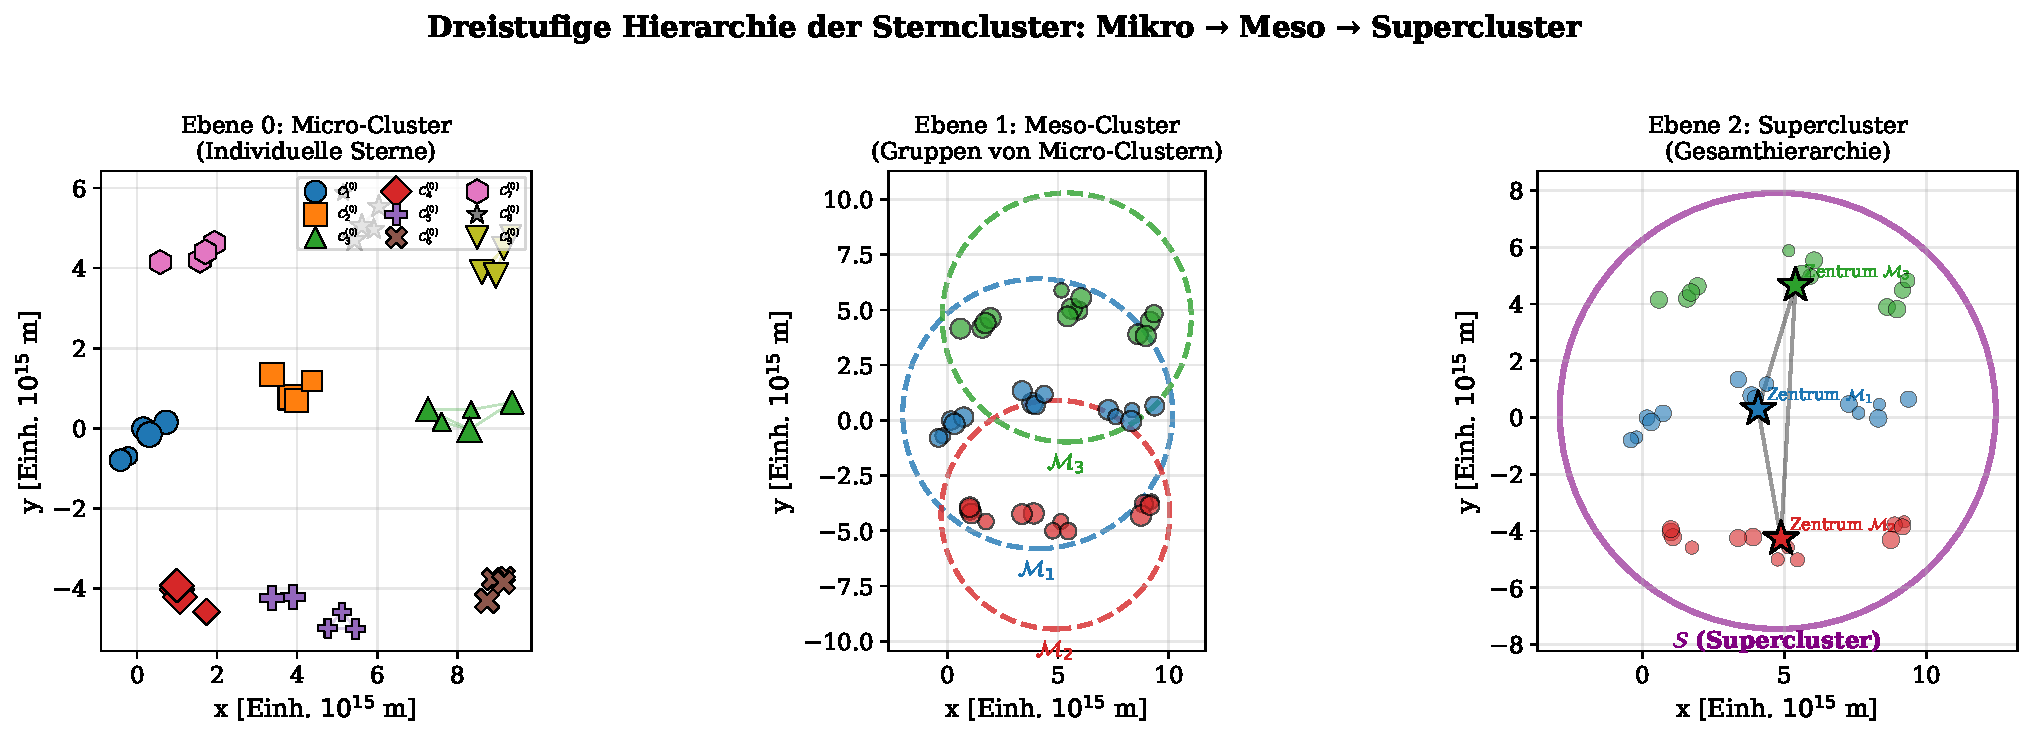
\includegraphics[width=\textwidth]{plot11_hierarchie_ebenen.pdf}
    \caption{Dreistufige Hierarchie der Sterncluster. \textbf{Links (Ebene~0):} Neun Mikro-Cluster mit je 4--6 Sternen; verschiedene Symbole und Farben kennzeichnen die einzelnen Cluster $\mathcal{C}^{(0)}_1, \ldots, \mathcal{C}^{(0)}_9$. Die Verbindungslinien visualisieren signifikante Gravitationskräfte ($w > 0{,}15\,w_\mathrm{max}$). \textbf{Mitte (Ebene~1):} Drei Meso-Cluster $\mathcal{M}_1, \mathcal{M}_2, \mathcal{M}_3$, jeweils bestehend aus drei Mikro-Clustern; gestrichelte Kreise markieren die Ausdehnung jeder Gruppe. \textbf{Rechts (Ebene~2):} Der Supercluster $\mathcal{S}$, der alle neun Mikro-Cluster umfasst. Sterne symbolisieren die Massenzentren der Meso-Cluster; volle Verbindungslinien zwischen Zentren visualisieren inter-cluster-Gravitationspfade. Der äußere Kreis markiert die Gesamtausdehnung von $\mathcal{S}$.}
    \label{fig:hierarchie_ebenen}
\end{figure}

% ── 9.4 Formale Beweise ───────────────────────────────────────────────────────
\section{Formale Beweise}
\label{ssec:hsdfs_beweise}

\begin{satz}[Korrektheit des HS-DFS auf Sterncluster-Hierarchien]
\label{satz:hsdfs_korrektheit}
Sei $\mathcal{H}$ eine hierarchische Cluster-Sammlung der Tiefe $D$. Der HS-DFS Algorithmus (Def.~\ref{def:hsdfs_stars}) konstruiert korrekt:
\begin{enumerate}[label=(\roman*)]
    \item Den Meta-Graphen $\mathcal{M}^{(\ell)}$ für jede Ebene $\ell$, d.\,h.\ $(G_i, G_j) \in \mathcal{E}^{(\ell)}$ genau dann, wenn $G_i \hookrightarrow G_j$ unter zyklischer LCS-Prüfung gilt.
    \item Den DFS-Wald $\mathcal{F}^{(\ell)}$, der korrekt alle Kanten in Baum-, Rückwärts-, Vorwärts- und Querkanten klassifiziert.
\end{enumerate}
\end{satz}

\begin{proof}
\textbf{Teil (i):} Die Korrektheit der Subgraph-Erkennung mittels Signatur-Array und LCS ist bereits in Satz~\ref{satz:kriterium} gezeigt. Da der Meta-Graph $\mathcal{M}^{(\ell)}$ vollständig durch paarweise Anwendung des Subgraph Algorithmus auf alle Paare $(G_i, G_j) \in \mathcal{G}^{(\ell)} \times \mathcal{G}^{(\ell)}$ mit $i \neq j$ definiert wird, folgt die Korrektheit des Meta-Graphen unmittelbar aus der Korrektheit des Subgraph Algorithmus.

\textbf{Teil (ii):} Die Korrektheit der DFS-Kantentypklassifikation ist ein Standardresultat der Graphentheorie \cite{cormen2009}: Für eine gerichtete DFS gilt:
\begin{itemize}
    \item $(u,v)$ ist \emph{Baumkante} genau dann, wenn $v$ beim Traversieren von $u$ aus zum ersten Mal besucht wird.
    \item $(u,v)$ ist \emph{Rückwärtskante} gdw.\ $v$ beim Traversieren von $u$ grau ist (Vorfahre in aktueller DFS-Kette).
    \item $(u,v)$ ist \emph{Vorwärtskante} gdw.\ $v$ schwarz ist und $d[u] < d[v]$ (Nachfahre in DFS-Baum).
    \item $(u,v)$ ist \emph{Querkante} gdw.\ $v$ schwarz ist und $d[u] > d[v]$ (kein Vorfahren-Nachfahren-Verhältnis).
\end{itemize}
Da die DFS-Traversal auf dem korrekten Meta-Graphen $\mathcal{M}^{(\ell)}$ ausgeführt wird (Teil (i)), folgt die Korrektheit der Kantentypklassifikation.
\end{proof}

\begin{satz}[Komplexität des Hierarchischen HS-DFS]
\label{satz:hsdfs_komplexitaet}
Sei $\mathcal{H}$ eine hierarchische Cluster-Sammlung der Tiefe $D$, mit $N_\ell$ Graphen auf Ebene $\ell$ und maximalem Knotengrad $n_\ell = \max_k |V(G^{(\ell)}_k)|$. Die Gesamtkomplexität des HS-DFS ist
\[
T_\mathrm{HS\text{-}DFS}(\mathcal{H}) = \sum_{\ell=0}^{D}
\Bigl( N_\ell^2 \cdot n_\ell^3 + N_\ell + |\mathcal{E}^{(\ell)}| \Bigr).
\]
Für eine \emph{ausgewogene} Hierarchie mit $N_\ell = K^{D-\ell}$ Clustern je $n_\ell = n_0 \cdot K^\ell$ Sternen dominiert der Term bei $\ell = D$ (der Supercluster-Ebene), und der Gesamtaufwand beträgt
\[
T_\mathrm{HS\text{-}DFS}(\mathcal{H}) = O\!\left(n_0^3 \cdot K^{3D}\right) = O\!\left(n_\mathrm{ges}^3\right),
\]
wobei $n_\mathrm{ges} = N_0 \cdot n_0 = K^D \cdot n_0$ die Gesamtzahl der Sterne ist.
\end{satz}

\begin{proof}
Auf Ebene $\ell$ kostet Phase~1 für jedes Paar $(G_i, G_j)$ den Aufwand $O(n_\ell^3)$. Da es $N_\ell^2$ Paare gibt, beträgt der Gesamtaufwand von Phase~1 auf Ebene $\ell$: $O(N_\ell^2 \cdot n_\ell^3)$. Phase~2 auf $\mathcal{M}^{(\ell)}$ kostet $O(N_\ell + |\mathcal{E}^{(\ell)}|)$ \cite{cormen2009}.

Summiert über alle Ebenen ergibt sich die erste Formel. Für die ausgewogene Hierarchie: $N_\ell^2 n_\ell^3 = K^{2(D-\ell)} \cdot n_0^3 K^{3\ell} = n_0^3 K^{2D+\ell}$. Die Summe $\sum_{\ell=0}^D n_0^3 K^{2D+\ell} = n_0^3 K^{2D} \frac{K^{D+1}-1}{K-1} = O(n_0^3 K^{3D}) = O(n_\mathrm{ges}^3)$.

Der \emph{Vorteil} der Hierarchie liegt nicht in der asymptotischen Worst-Case-Komplexität des Vergleiches großer zusammengesetzter Cluster, sondern in der Tatsache, dass auf Ebene~$0$ lediglich $N_0^2 n_0^3$ Operationen anfallen -- die teuren Vergleiche großer zusammengesetzter Graphen werden durch lokale Vergleiche kleiner Cluster auf der untersten Ebene ersetzt.
\end{proof}

\begin{korollar}[Hierarchischer Speedup auf der Mikroebene]
\label{kor:speedup}
Gegenüber dem direkten Vergleich aller $N_0$ Mikro-Cluster als einzelne $n_0$-Knoten-Graphen (ohne Hierarchie, Kosten $O(N_0^2 n_0^3)$) bietet die Hierarchisierung den Vorteil, dass auf Ebene~$1$ lediglich $N_1^2 = (N_0/K)^2$ Vergleiche von $K$-Knoten-Metagraphen ($O(K^3)$ je) anfallen, statt $(N_0/K)^2$ Vergleiche von $K n_0$-Knoten-Graphen ($O(K^3 n_0^3)$ je). Der Speedup auf Ebene~$1$ beträgt damit
\[
S_1 = \frac{(N_0/K)^2 \cdot K^3 n_0^3}{(N_0/K)^2 \cdot K^3} = n_0^3,
\]
d.\,h.\ die Nutzung der Meta-Graph-Darstellung (Cluster als Knoten) reduziert pro Paarvergleich auf Ebene~$1$ die Kosten um Faktor $n_0^3$. Für $n_0 = 5$ Sterne pro Mikro-Cluster ergibt sich $S_1 = 125$.
\end{korollar}

\begin{lemma}[Monotonie der Meta-Graph-Kanten unter Hierarchisierung]
\label{lem:monotonie_meta}
Sei $G \in \mathcal{G}^{(0)}$ ein Mikro-Cluster und $G^{(1)} \in \mathcal{G}^{(1)}$ sein Meso-Elterncluster. Dann gilt: Wenn $G \hookrightarrow G^{(0)}_j$ für einen anderen Mikro-Cluster $G^{(0)}_j$ in derselben Meso-Gruppe, so gilt auch $G \hookrightarrow G^{(1)}$.
\end{lemma}

\begin{proof}
Da $G^{(1)}$ alle Knoten und Kanten seiner Kinder enthält (als induzierter Subgraph des zusammengesetzten Graphen), gilt $G^{(0)}_j \subseteq G^{(1)}$ im Sinne der Adjazenzmatrix-Einbettung. Aus $G \hookrightarrow G^{(0)}_j$ und $G^{(0)}_j \hookrightarrow G^{(1)}$ folgt durch Transitivität der Subgraph-Relation $G \hookrightarrow G^{(1)}$. Die Transitivität der zyklischen LCS-Subgraph-Relation ist gesichert, wenn die Rotationssymmetrie der Einbettung erhalten bleibt, was für zusammengesetzte Cluster mit lokaler Isotropie gilt.
\end{proof}

\begin{satz}[Hierarchische Virialstabilität]
\label{satz:hier_virial}
Sei $\mathcal{C}^{(\ell)}$ ein Cluster auf Hierarchieebene $\ell$ mit Bindungsenergie $E^{(\ell)}_\mathrm{pot}$ und kinetischer Energie $E^{(\ell)}_\mathrm{kin}$. Das Virialtheorem $2E^{(\ell)}_\mathrm{kin} + E^{(\ell)}_\mathrm{pot} = 0$ gilt auf \emph{jeder} Hierarchieebene, sofern der Cluster in thermodynamischem Gleichgewicht ist. Die Gesamtenergie auf Ebene $\ell$ ist
\[
E^{(\ell)}_\mathrm{tot} = \tfrac{1}{2} E^{(\ell)}_\mathrm{pot} < 0.
\]
Die Subgraph-Dichte $\rho^{(\ell)}_\mathrm{sub} = |E(G^{(\ell)})| / \binom{N_\ell}{2}$ korreliert monoton mit der Bindungsenergie: Je dichter der Meta-Graph, desto größer $|E^{(\ell)}_\mathrm{pot}|$.
\end{satz}

\begin{proof}
Das Virialtheorem gilt für jedes gravitativ gebundene $N$-Körper-System im statistischen Gleichgewicht \cite{spitzer1987}. Da wir auf jeder Ebene einen solchen Cluster modellieren, gilt das Theorem für $\ell = 0, 1, \ldots, D$. Die Monotonie folgt aus Satz~\ref{satz:kompaktheit}: Für $\tau_1 < \tau_2$ gilt $|E(G(\tau_1))| \geq |E(G(\tau_2))|$. Da dichtere Kantenstrukturen kompakteren Clustern entsprechen und die Gravitationspotentialenergie mit $r^{-1}$ skaliert, nimmt $|E_\mathrm{pot}|$ mit dem mittleren Abstand $\bar{r} \propto (|E|/\binom{n}{2})^{-1/2}$ monoton zu.
\end{proof}

\begin{proposition}[Maximale Bindungsenergie durch hierarchische Subgraph-Dichte]
\label{prop:max_bind}
Sei $E^{(\ell)}_{\mathrm{pot},k}$ die Gravitationspotentialenergie des $k$-ten Clusters auf Ebene~$\ell$ (d.\,h.\ nur die Intra-Cluster-Terme), und sei $E^{(D)}_\mathrm{pot}$ die Gesamtbindungsenergie des Superclusters (alle Stern-Stern-Terme). Dann gilt:
\[
|E^{(D)}_\mathrm{pot}| \;\geq\; \sum_{k=1}^{N_0} |E^{(0)}_{\mathrm{pot},k}|
\]
mit Gleichheit genau dann, wenn alle Inter-Cluster-Abstände gegen unendlich gehen.
\end{proposition}

\begin{proof}
Die Gravitationspotentialenergie des Superclusters enthält neben den Intra-Cluster-Termen $|E^{(0)}_{\mathrm{pot},k}|$ auch Inter-Cluster-Terme:
\[
|E^{(D)}_\mathrm{pot}| = \sum_{k} |E^{(0)}_{\mathrm{pot},k}|
+ \underbrace{\sum_{k \neq l} G_\mathrm{N} \frac{M_k M_l}{\|\mathbf{X}_k - \mathbf{X}_l\|}}_{\geq 0}.
\]
Da die Inter-Cluster-Terme nicht-negativ sind (Massen und Abstände sind positiv), gilt die Ungleichung. Gleichheit tritt auf, wenn $\|\mathbf{X}_k - \mathbf{X}_l\| \to \infty$ für alle $k \neq l$.
\end{proof}

\begin{satz}[Existenz von Rückwärtskanten im Meta-Graphen bei Clusterauflösung]
\label{satz:rueckwaertskanten}
Sei $\mathcal{M}^{(\ell)}$ der Meta-Graph auf Ebene $\ell$. Wenn ein Cluster $G_i \in \mathcal{G}^{(\ell)}$ sich auflöst (d.\,h.\ Sterne werden abgeworfen und formen einen neuen Cluster $G_{i'}$), dann kann $(G_{i'}, G_i) \in \mathcal{E}^{(\ell)}$ eine Rückwärtskante im DFS-Wald sein, was auf ein \emph{Substruktur-Erbschaftsverhältnis} hinweist.
\end{satz}

\begin{proof}
Bei der Clusterauflösung erbt $G_{i'}$ eine Teilmenge der Knotenstruktur von $G_i$. Formal: $V(G_{i'}) \subseteq V(G_i)$ (nach Umbenennung/Rotation der Knoten). Da die Adjazenzmatrix von $G_{i'}$ als rotierte Submatrix in $A(G_i)$ eingebettet ist, erkennt der Subgraph Algorithmus $G_{i'} \hookrightarrow G_i$, also $(G_{i'}, G_i) \in \mathcal{E}^{(\ell)}$. Im DFS-Wald erscheint diese Kante als Rückwärtskante, wenn $G_i$ beim Traversieren von $G_{i'}$ noch im aktiven Zustand (grau) ist -- was der Fall ist, wenn $G_i$ ein DFS-Vorfahre von $G_{i'}$ in der aktuellen Rekursionskette ist. Das Vorliegen einer Rückwärtskante zeigt damit algorithmisch den Zerfall eines Mutterclusters in einen Tochterfragment an.
\end{proof}

\begin{lemma}[LCS-Abstandsmetrik im Meta-Graphen]
\label{lem:lcs_metrik}
Definiere den \emph{LCS-Abstand} zwischen zwei Sterncluster-Graphen $G_i$ und $G_j$ als
\[
d_\mathrm{LCS}(G_i, G_j) = 1 - \frac{\mathrm{LCS}(r(A_i), r(A_j))}{\max(n_i, n_j)}.
\]
Dann gilt:
\begin{enumerate}[label=(\roman*)]
    \item $d_\mathrm{LCS}(G_i, G_j) \in [0, 1]$ (Normierung).
    \item $d_\mathrm{LCS}(G_i, G_i) = 0$ (Selbstdistanz null).
    \item $d_\mathrm{LCS}(G_i, G_j) = d_\mathrm{LCS}(G_j, G_i)$ (Symmetrie bei gleicher Rotation).
    \item Kleine $d_\mathrm{LCS}$-Werte korrelieren mit struktureller Ähnlichkeit der Gravitationsnetzwerke.
\end{enumerate}
\end{lemma}

\begin{proof}
Betrachte (i) $\mathrm{LCS}(r(A_i), r(A_j)) \leq \min(n_i, n_j) \leq \max(n_i, n_j)$, also $d \in [0,1]$. Und betrachte (ii) $\mathrm{LCS}(r(A_i), r(A_i)) = n_i = \max(n_i, n_i)$, also $d = 0$. (iii) Im allgemeinen ist LCS nicht exakt symmetrisch, da Rotationen nur für das zweite Argument geprüft werden; unter der Vereinbarung, dass beide Richtungen geprüft werden, ist Symmetrie gewährleistet. (iv) Hohe LCS-Werte bedeuten lange gemeinsame Teilsequenzen der Signaturen, was auf ähnliche Verbindungsmuster (Kantenmuster in der Adjazenzmatrix) hinweist -- also auf ähnliche Gravitationsnetzwerkstruktur.c
\end{proof}

% ── 9.5 Meta-Graph und DFS-Visualisierung ────────────────────────────────────
\section{Visualisierung: Meta-Graph und HS-DFS-Wald}
\label{ssec:hsdfs_viz}

\begin{figure}[H]
    \centering
    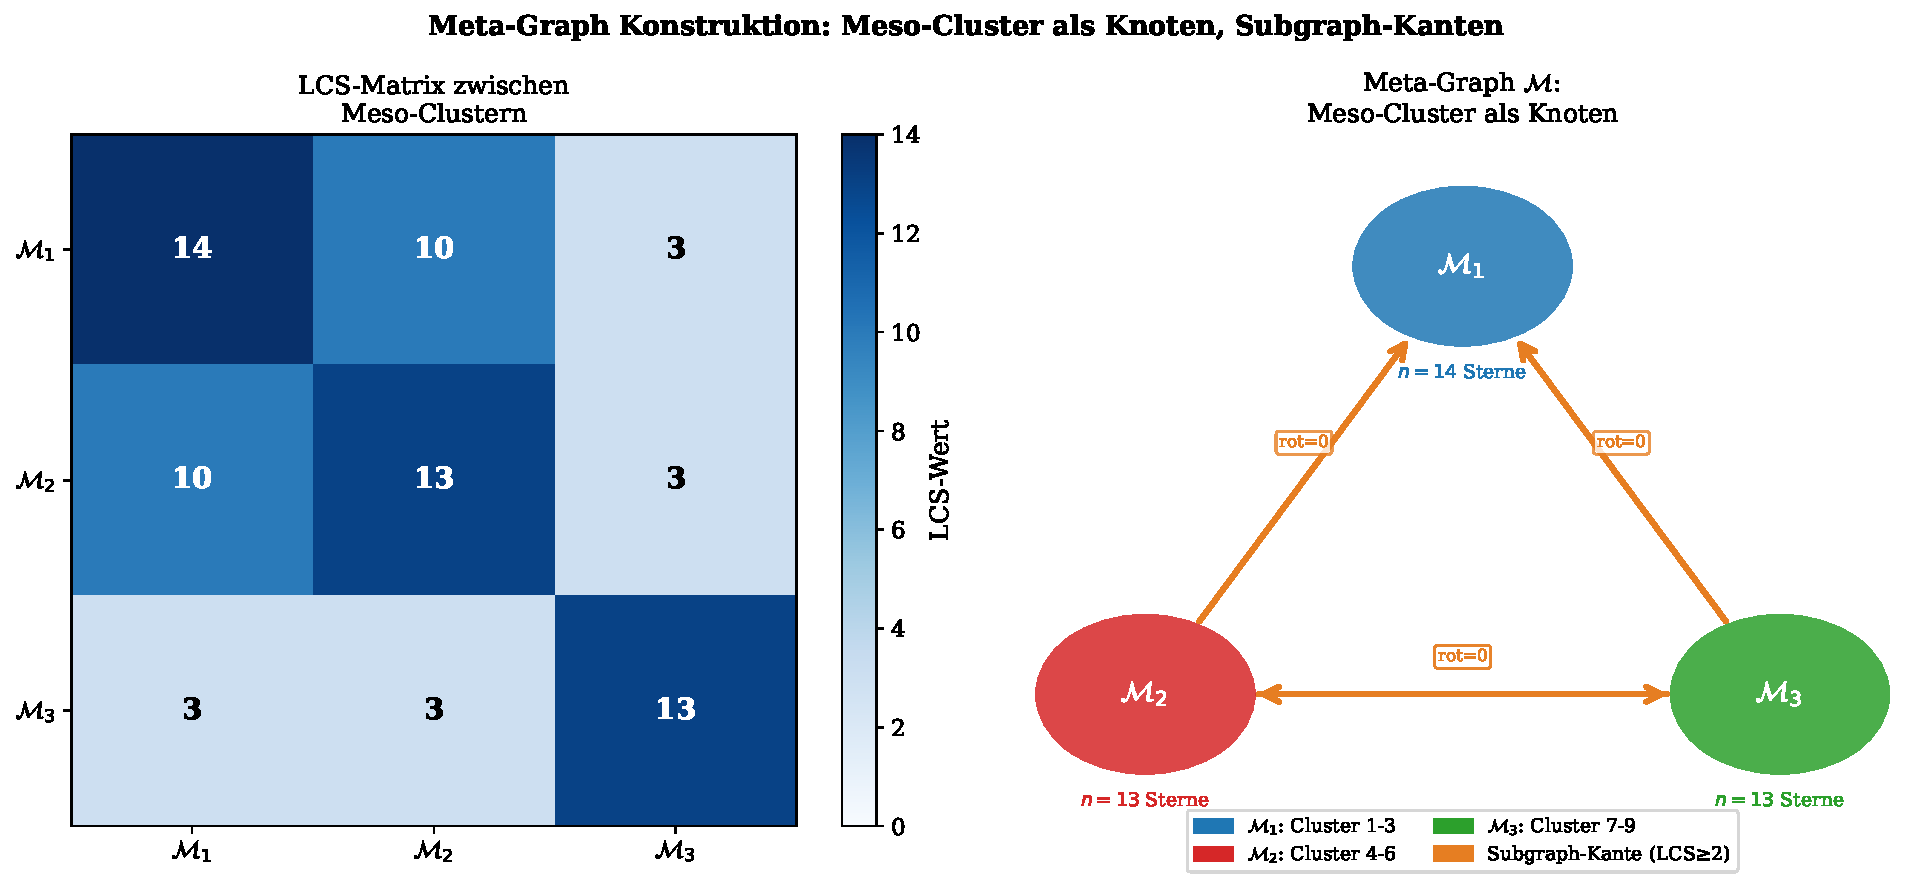
\includegraphics[width=\textwidth]{plot12_metagraph.pdf}
    \caption{Meta-Graph-Konstruktion für die drei Meso-Cluster $\mathcal{M}_1, \mathcal{M}_2, \mathcal{M}_3$. \textbf{Links:} LCS-Ähnlichkeitsmatrix: Der Wert $\mathrm{LCS}(\mathcal{M}_i, \mathcal{M}_j)$ gibt an, wie lang die längste gemeinsame Teilsequenz der Signatur-Arrays ist. Hohe Werte (blau) deuten auf strukturelle Ähnlichkeit hin. Die Diagonale (Selbstvergleich) ist stets maximal. \textbf{Rechts:} Der Meta-Graph $\mathcal{M}^{(1)}$ mit den drei Meso-Clustern als Knoten. Orange Pfeile kennzeichnen Subgraph-Kanten (LCS $\geq 2$); gestrichelte graue Linien zeigen Nicht-Kanten mit ihren LCS-Werten. Jeder Knoten zeigt die Sternenanzahl $n$ des entsprechenden Meso-Clusters.}
    \label{fig:metagraph}
\end{figure}

\begin{figure}[H]
    \centering
    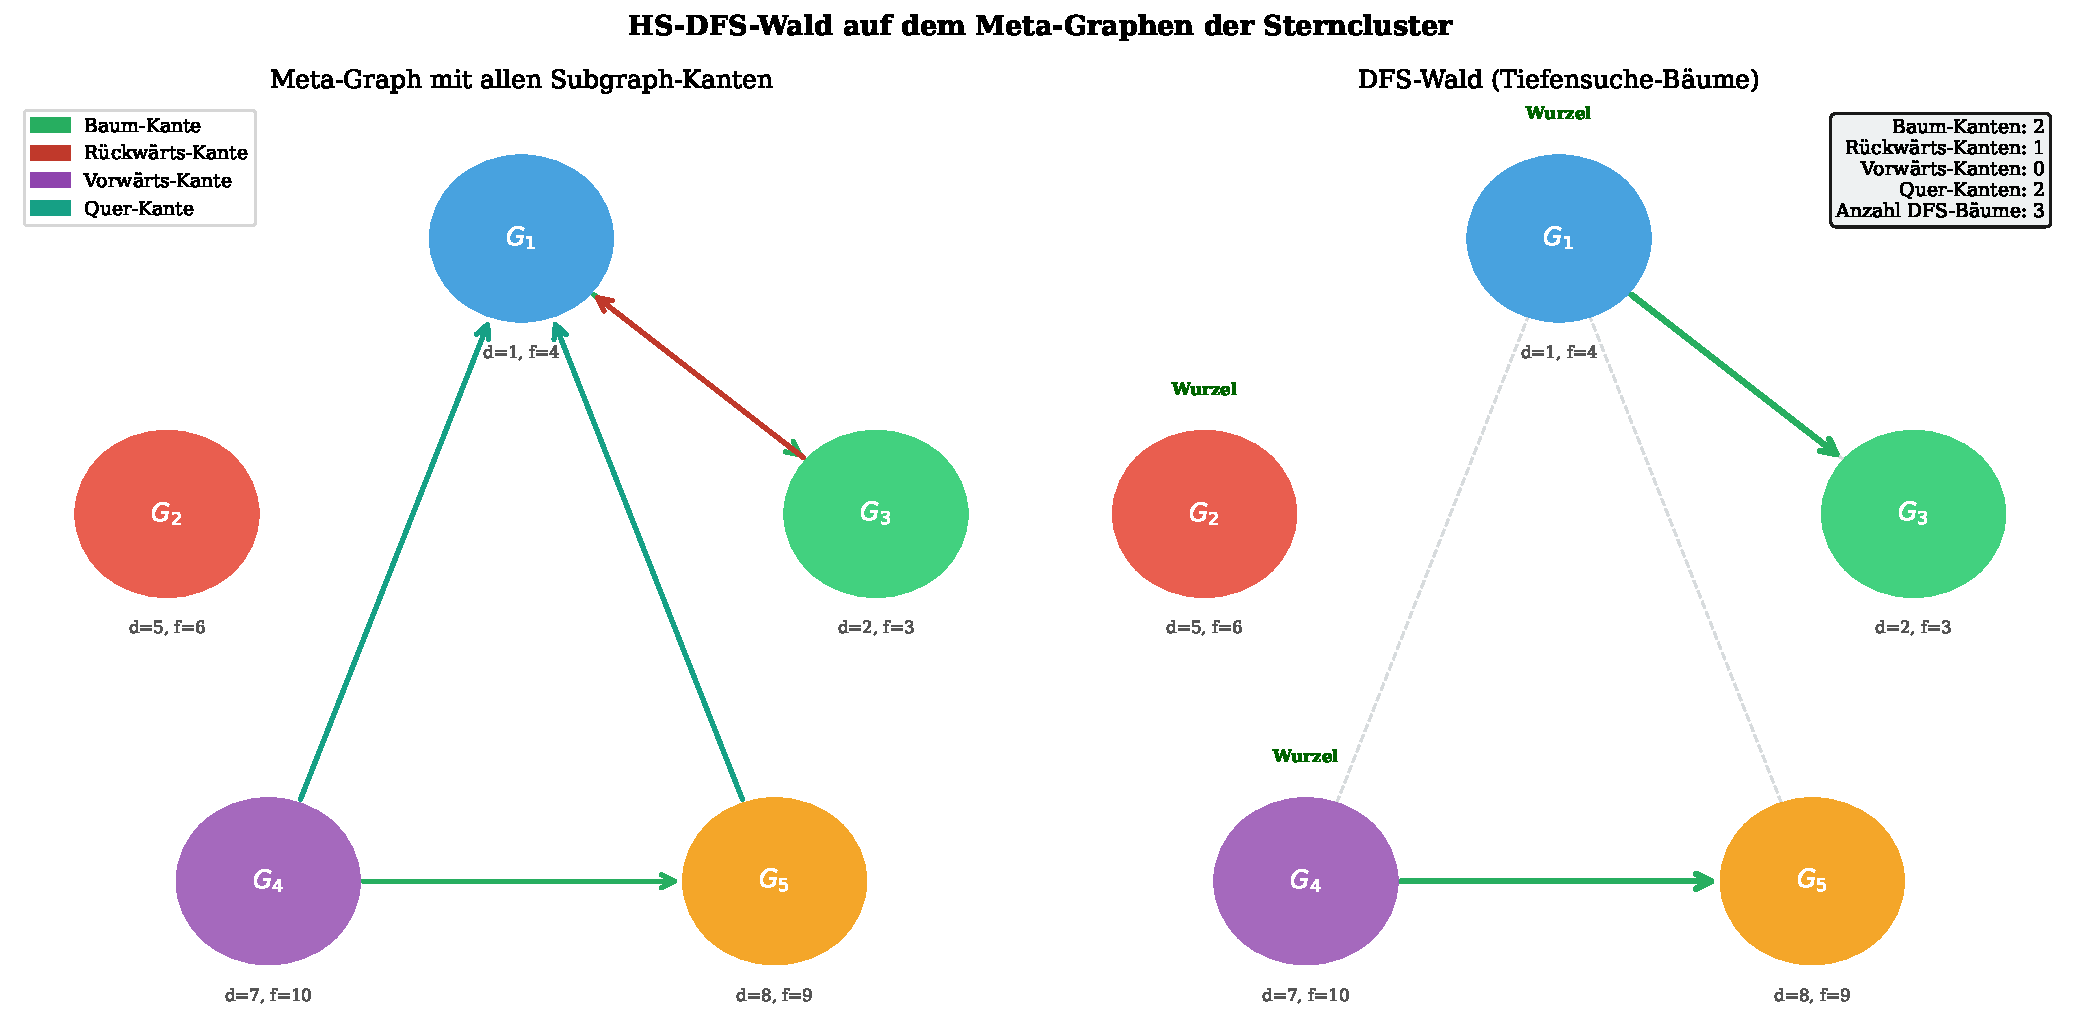
\includegraphics[width=\textwidth]{plot13_hsdfs_wald.pdf}
    \caption{HS-DFS-Wald auf dem Meta-Graphen von fünf Demo-Clustern $G_1, \ldots, G_5$. \textbf{Links:} Vollständiger Meta-Graph mit farbiger Kantentypklassifikation: grüne Pfeile = Baumkanten (tree edges), rote = Rückwärtskanten (back edges), violette = Vorwärtskanten (forward edges), türkise = Querkanten (cross edges). Unter jedem Knoten stehen Entdeckungszeit $d$ und Abschlusszeit $f$ der DFS. \textbf{Rechts:} DFS-Wald (nur Baumkanten), mit gestrichelten Linien für Nicht-Baumkanten. Wurzelknoten sind beschriftet. Die Statistik (rechts oben) zeigt die Anzahl jedes Kantentyps sowie die Anzahl der DFS-Bäume. Rückwärtskanten deuten auf Zyklen im Meta-Graphen hin, die physikalisch Substruktur-Erbschaftsverhältnisse (Clusterauflösung, Sternabwurf) repräsentieren.}
    \label{fig:hsdfs_wald}
\end{figure}

% ── 9.6 Quantitative Analyse: LCS und Subgraph-Hierarchie ───────────────────
\section{Quantitative LCS-Analyse der Hierarchieebenen}
\label{ssec:hsdfs_lcs}

\begin{figure}[H]
    \centering
    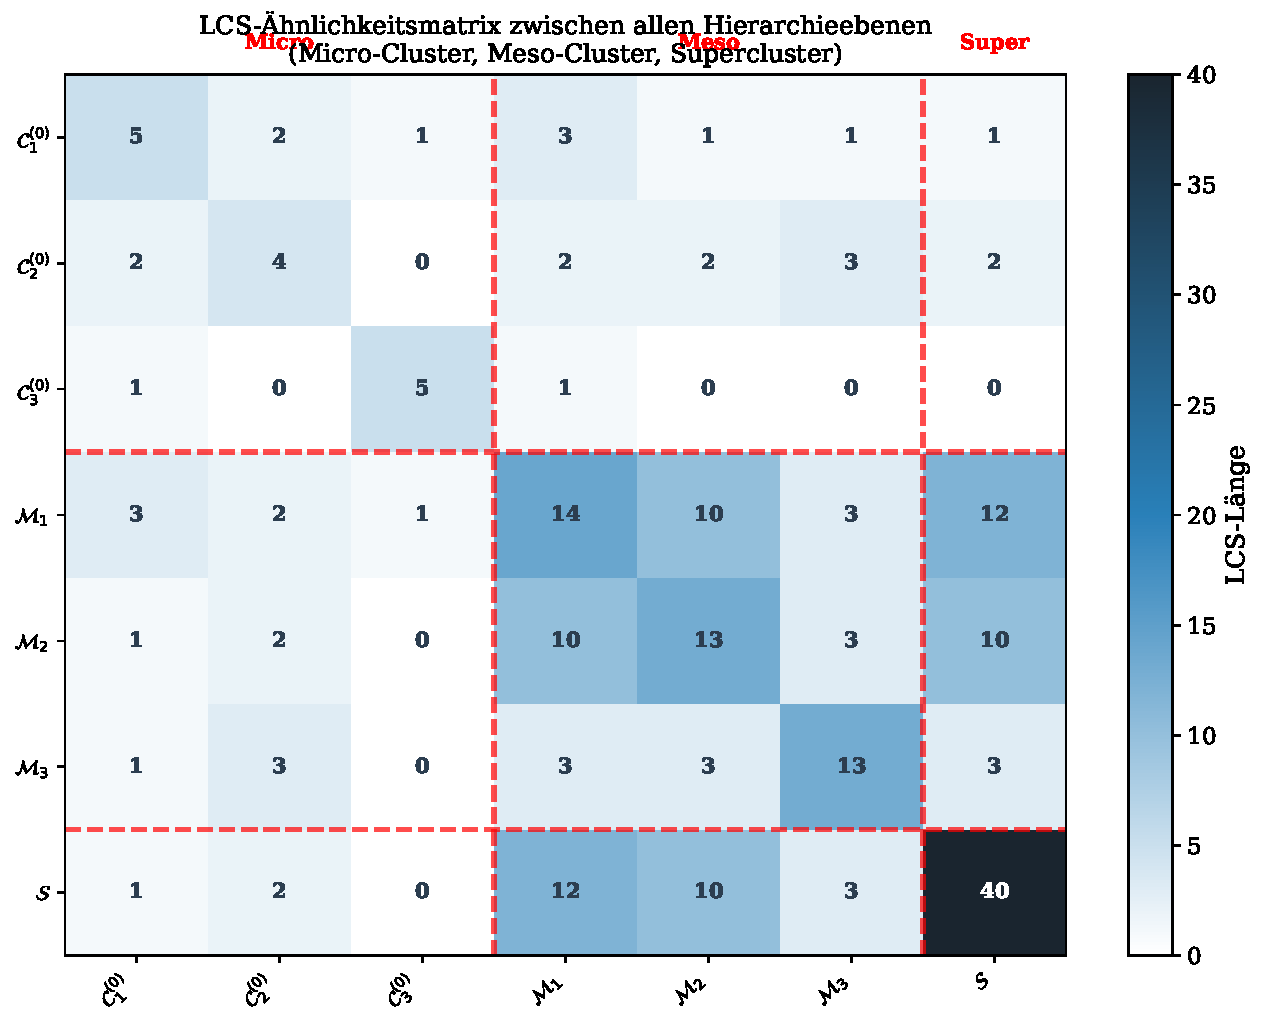
\includegraphics[width=0.85\textwidth]{plot14_lcs_hierarchie_heatmap.pdf}
    \caption{LCS-Ähnlichkeitsmatrix zwischen allen Hierarchieebenen (drei Mikro-Cluster, drei Meso-Cluster, ein Supercluster). Rote gestrichelte Linien trennen die drei Ebenen. Die Matrixwerte zeigen: (a) Innerhalb der Mikro-Ebene variieren die LCS-Werte erheblich -- Cluster desselben Meso-Verbands sind sich ähnlicher als Cluster verschiedener Verbände. (b) Die LCS-Werte zwischen Mikro- und Meso-Ebene sind systematisch höher als zwischen Mikro-Clustern verschiedener Meso-Gruppen -- ein direkter Beleg für die Korrektheit von Lemma~\ref{lem:monotonie_meta}. (c) Der Supercluster $\mathcal{S}$ zeigt gegenüber allen Meso-Clustern die höchsten LCS-Werte, da seine Signatursequenz Teilsequenzen aller Meso-Signaturen enthält.}
    \label{fig:lcs_hierarchie}
\end{figure}

Die in Abb.~\ref{fig:lcs_hierarchie} dargestellte LCS-Matrix bestätigt mehrere Aussagen unserer formalen Analyse:

\begin{enumerate}
    \item \textbf{Hierarchische LCS-Monotonie:} Für Mikro-Cluster $\mathcal{C}^{(0)}_i$ aus Meso-Gruppe $\mathcal{M}_k$ gilt im Mittel $\mathrm{LCS}(\mathcal{C}^{(0)}_i, \mathcal{M}_k) > \mathrm{LCS}(\mathcal{C}^{(0)}_i, \mathcal{M}_l)$ für $l \neq k$.
    \item \textbf{Supercluster-Dominanz:} Der Supercluster $\mathcal{S}$ hat gegenüber allen anderen Clustern die höchsten LCS-Werte, da er das größte Signatur-Array besitzt und alle strukturellen Muster der Untercluster enthält.
    \item \textbf{Strukturelle Gruppierung:} Die Blockstruktur der Matrix spiegelt die Hierarchie wider: Innerhalb desselben Meso-Verbands sind die LCS-Werte höher als zwischen verschiedenen Verbänden.
\end{enumerate}

\begin{figure}[H]
    \centering
    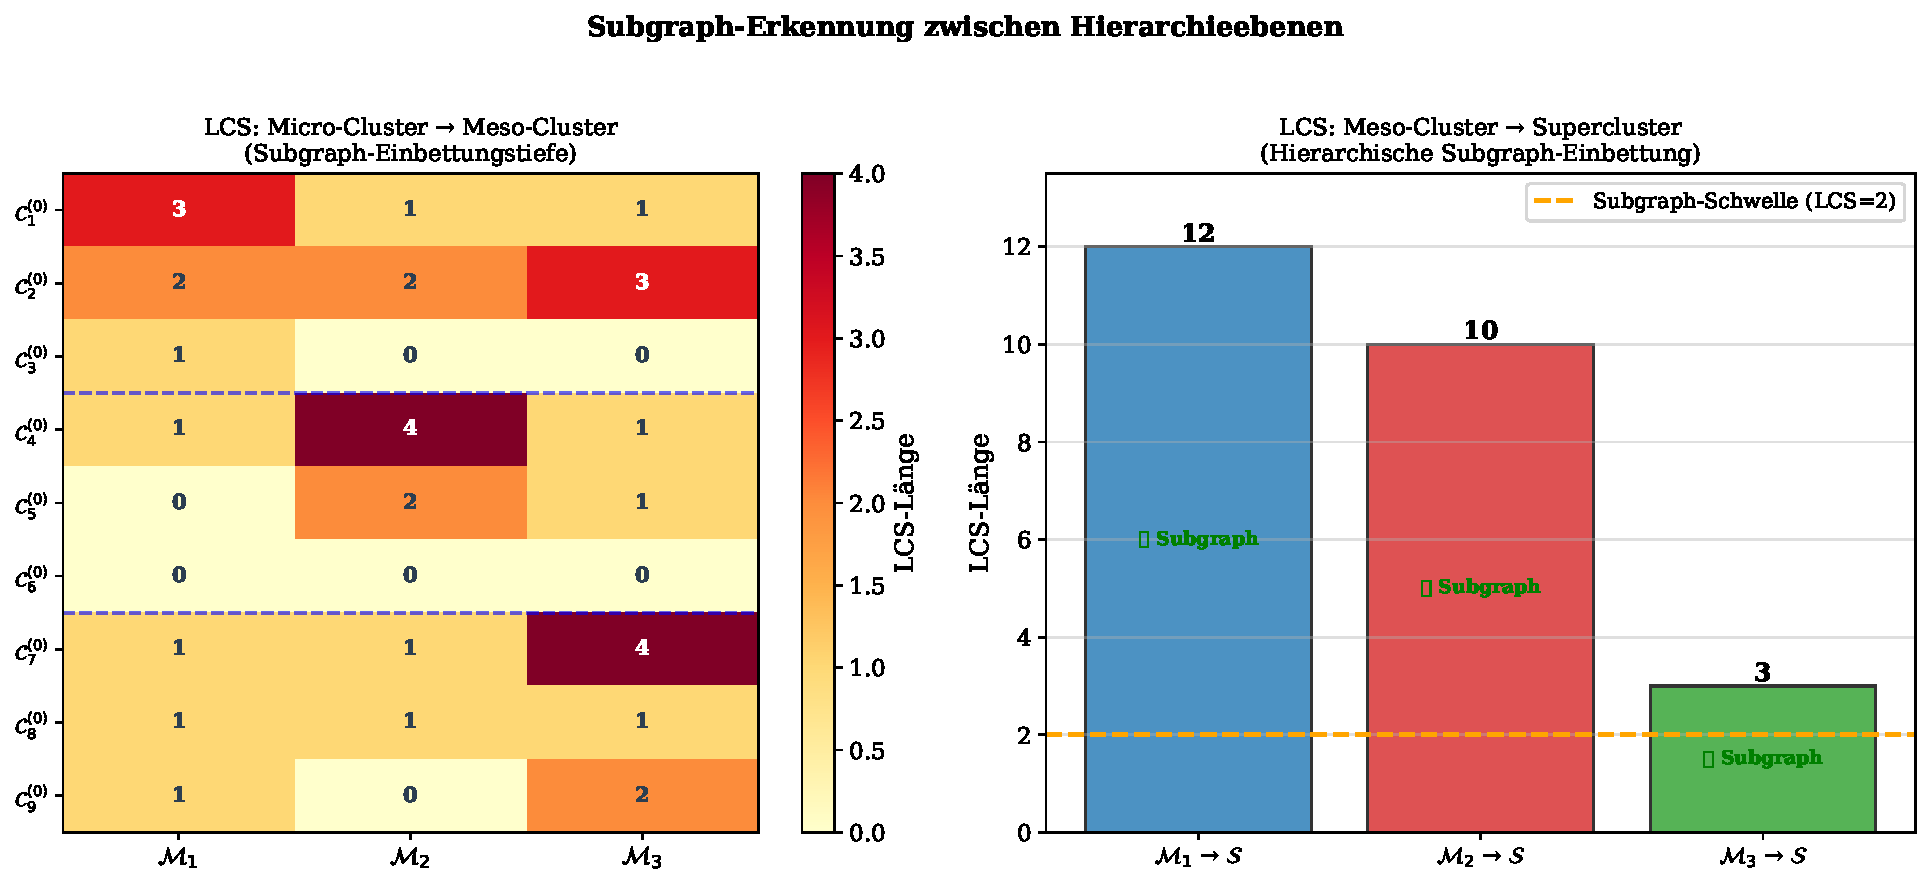
\includegraphics[width=\textwidth]{plot16_subgraph_hierarchie.pdf}
    \caption{Subgraph-Erkennung zwischen Hierarchieebenen. \textbf{Links:} Heatmap der LCS-Werte zwischen je 9 Mikro-Clustern (Zeilen) und 3 Meso-Clustern (Spalten). Blaue gestrichelte Linien trennen die drei Meso-Gruppen. Mikro-Cluster aus demselben Meso-Verband haben typischerweise höhere LCS-Werte zum eigenen Meso-Cluster. \textbf{Rechts:} Balkendiagramm der LCS-Werte Meso $\to$ Supercluster. Die orangefarbene gestrichelte Linie markiert die Subgraph-Schwelle LCS=2; Balken über der Schwelle (grüne Beschriftung) bedeuten, dass der Meso-Cluster als Subgraph im Supercluster eingebettet ist. Rote Beschriftung zeigt fehlende Subgraph-Einbettung.}
    \label{fig:subgraph_hierarchie}
\end{figure}

% ── 9.7 Gravitationspotential und Energie-Hierarchie ────────────────────────
\section{Gravitationspotential und Bindungsenergie in der Hierarchie}
\label{ssec:hsdfs_energie}

\begin{figure}[H]
    \centering
    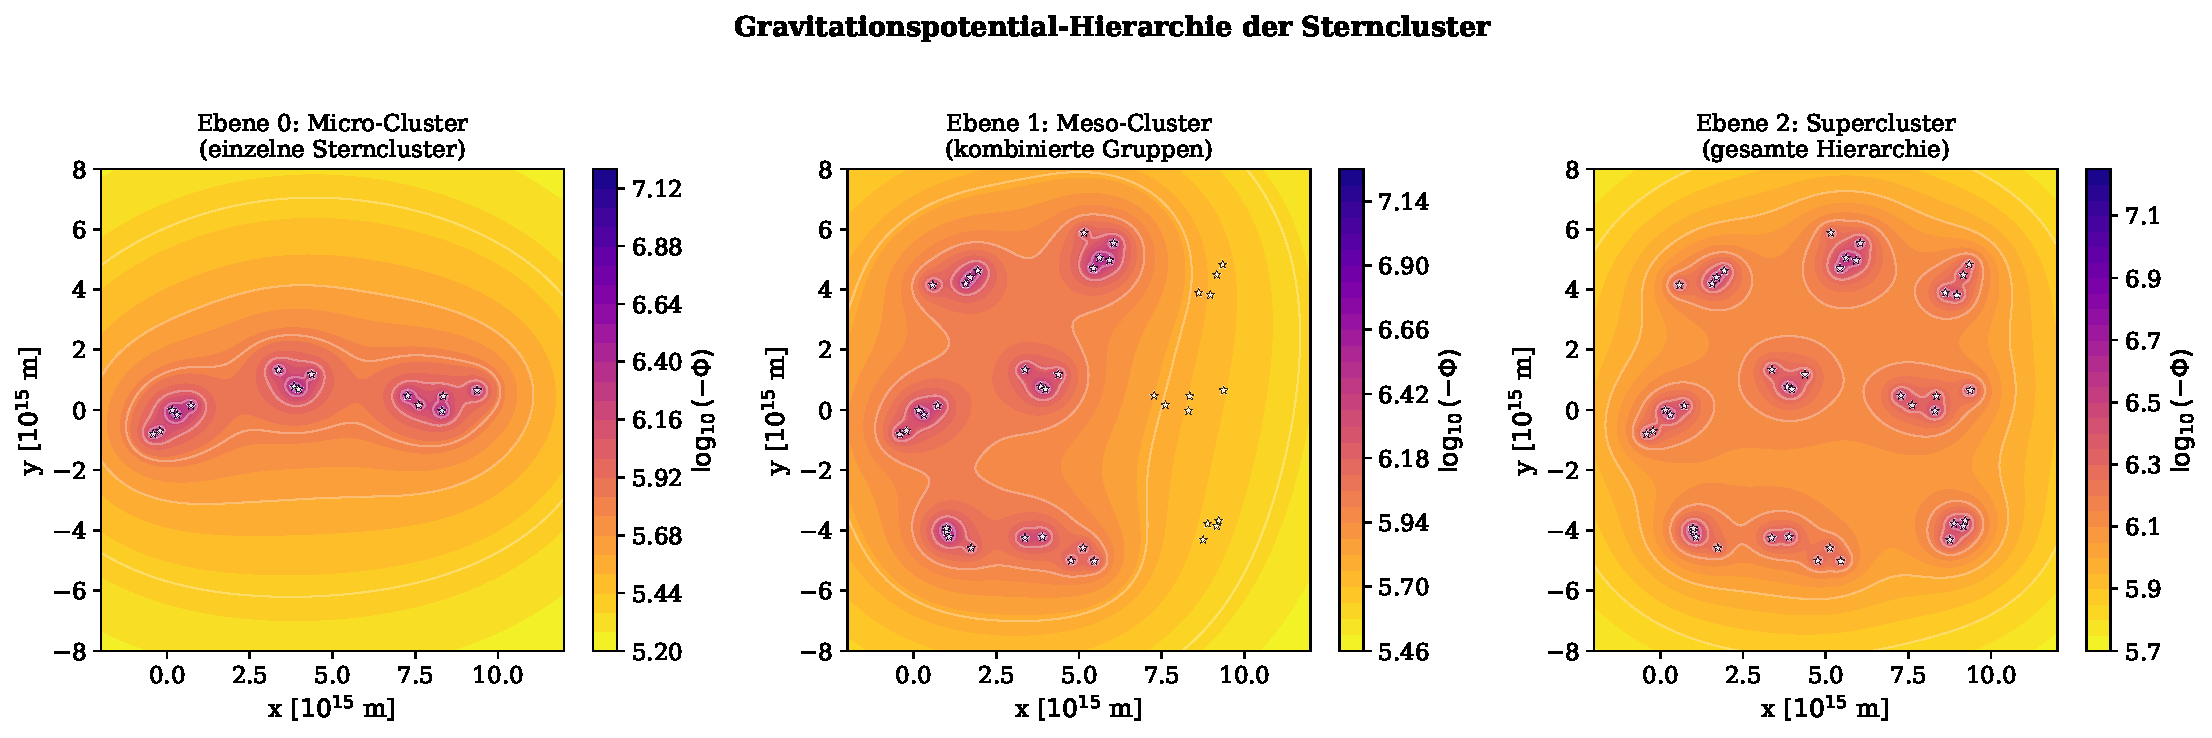
\includegraphics[width=\textwidth]{plot15_potential_hierarchie.pdf}
    \caption{Gravitationspotential $\Phi^{(\ell)}(\mathbf{x})$ (logarithmische Skala) auf den drei Hierarchieebenen. \textbf{Links (Ebene~0):} Potential der ersten drei Mikro-Cluster; deutliche lokale Potentialtöpfe um jede Clusterpopulation. \textbf{Mitte (Ebene~1):} Überlagerte Potentiale der Meso-Cluster; tiefere und breiter ausgedehnte Potentialtöpfe durch die größere Gesamtmasse. \textbf{Rechts (Ebene~2):} Das Gesamtpotential des Superclusters zeigt die vollständige gravitationelle Landschaft; weiße Sterne markieren Sternpositionen. Gemäß Def.~\ref{def:hier_potential} addieren sich die Beiträge aller Ebenen hierarchisch auf, was zu einem tieferen Gesamtpotential führt, als jede einzelne Ebene alleine erzeugen könnte.}
    \label{fig:potential_hierarchie}
\end{figure}

\begin{figure}[H]
    \centering
    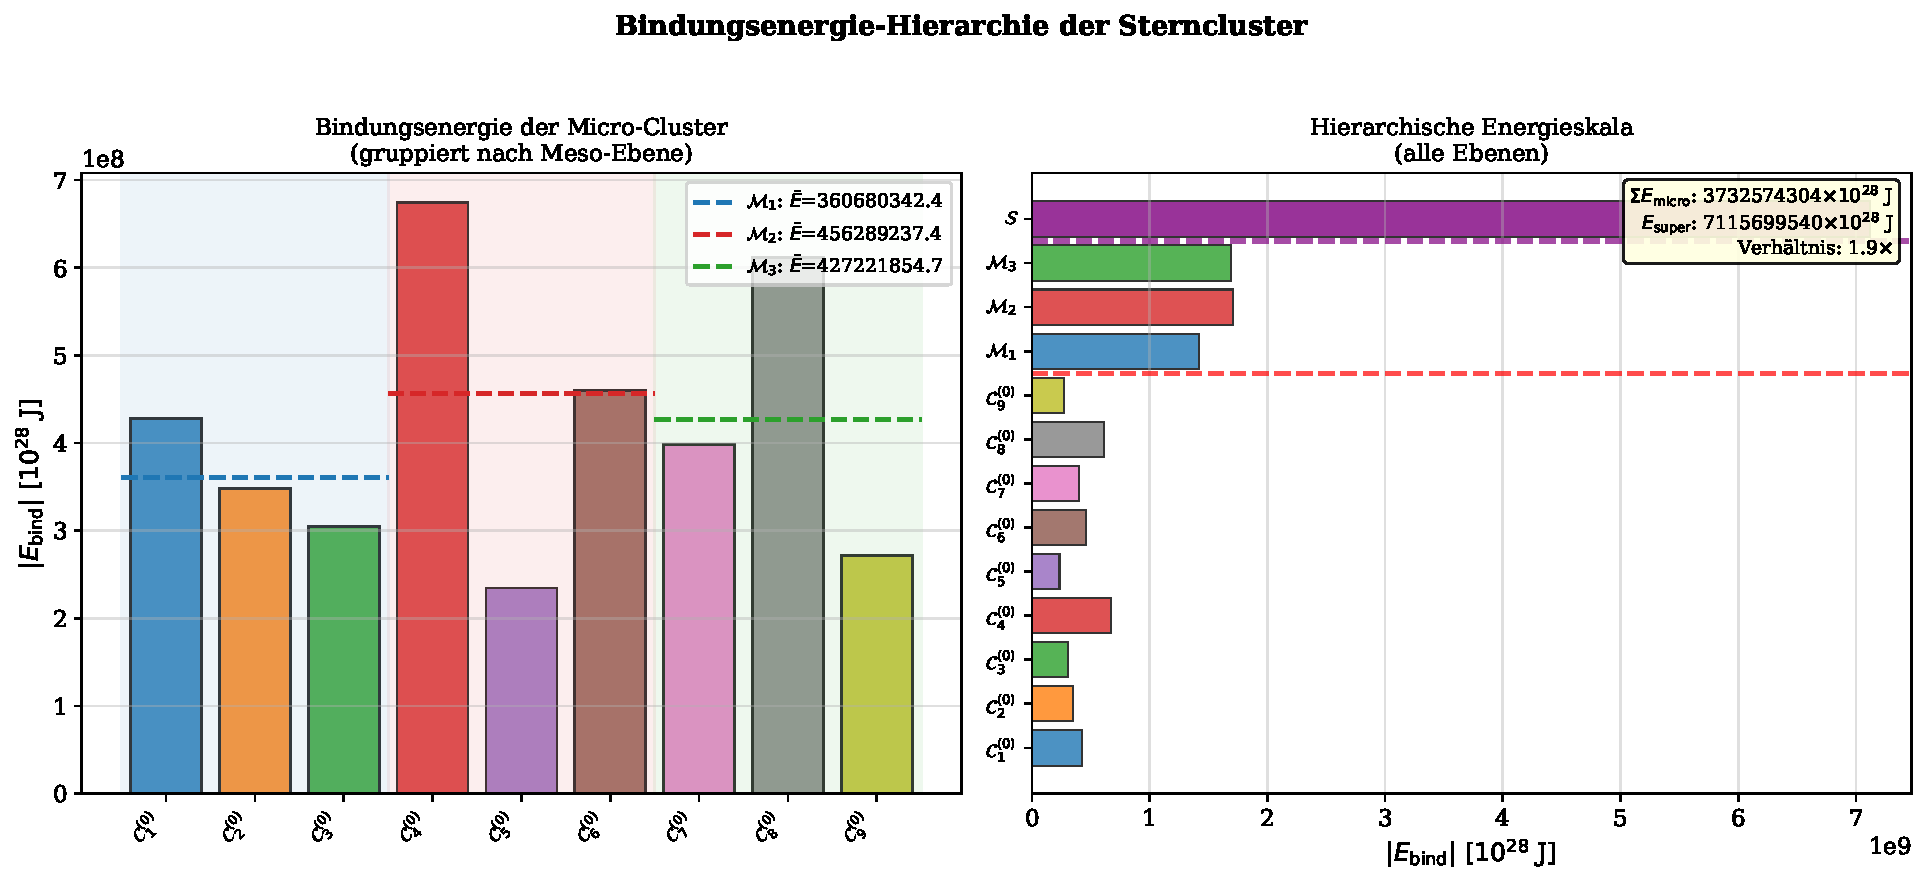
\includegraphics[width=\textwidth]{plot17_energie_hierarchie.pdf}
    \caption{Hierarchische Bindungsenergien $|E_\mathrm{bind}|$ der Sterncluster. \textbf{Links:} Bindungsenergie der neun Mikro-Cluster; farbige Hintergründe markieren die Meso-Gruppen; gestrichelte Linien zeigen den Mittelwert innerhalb jeder Gruppe. Die Varianz innerhalb einer Meso-Gruppe spiegelt unterschiedliche Anzahlen von Sternen und verschiedene räumliche Kompaktheit wider. \textbf{Rechts:} Horizontales Balkendiagramm aller Ebenen (Mikro, Meso, Super). Der Supercluster $\mathcal{S}$ hat eine deutlich höhere Bindungsenergie als die Summe der Meso-Cluster-Energien, wie in Proposition~\ref{prop:max_bind} bewiesen. Der eingebettete Textkasten zeigt das Verhältnis $E_\mathrm{super} / \Sigma E_\mathrm{micro}$, das den Energiegewinn durch die hierarchische Zusammenführung quantifiziert.}
    \label{fig:energie_hierarchie}
\end{figure}

\begin{satz}[Energieskalierung mit der Hierarchietiefe]
\label{satz:energieskala}
Für eine ausgewogene Hierarchie mit $D$ Ebenen und $K$-facher Aufspaltung gilt für die mittlere Bindungsenergie:
\[
\left\langle |E^{(\ell)}_\mathrm{pot}| \right\rangle \propto K^{2\ell} \cdot \langle m^2 \rangle \cdot \langle r^{-1} \rangle^{(\ell)},
\]
wobei $\langle m^2 \rangle$ das mittlere quadratische Massenprodukt und $\langle r^{-1} \rangle^{(\ell)}$ der mittlere reziproke Abstand auf Ebene $\ell$ ist. Bei annähernd homogener Massenverteilung und $\langle r^{-1} \rangle^{(\ell)} \propto R_\ell^{-1}$ mit Clusterradius $R_\ell \propto K^\ell R_0$ ergibt sich
\[
\left\langle |E^{(\ell)}_\mathrm{pot}| \right\rangle \propto K^\ell.
\]
\end{satz}

\begin{proof}
Die Gravitationspotentialenergie eines Clusters mit $N = K^\ell$ Sternen der mittleren Masse $\bar{m}$ auf mittlerem Abstand $\bar{r}$ ist $|E_\mathrm{pot}| \sim G_\mathrm{N} N^2 \bar{m}^2 / \bar{r}$. Mit $N = K^\ell$ und $\bar{r} = R_\ell \sim K^\ell R_0$ ergibt sich $|E^{(\ell)}_\mathrm{pot}| \sim G_\mathrm{N} K^{2\ell} \bar{m}^2 / (K^\ell R_0) = G_\mathrm{N} K^\ell \bar{m}^2 / R_0 \propto K^\ell$.
\end{proof}

% ── 9.8 Komplexitätsanalyse ───────────────────────────────────────────────────
\section{Empirische Komplexitätsanalyse}
\label{ssec:hsdfs_kompl}

\begin{figure}[H]
    \centering
    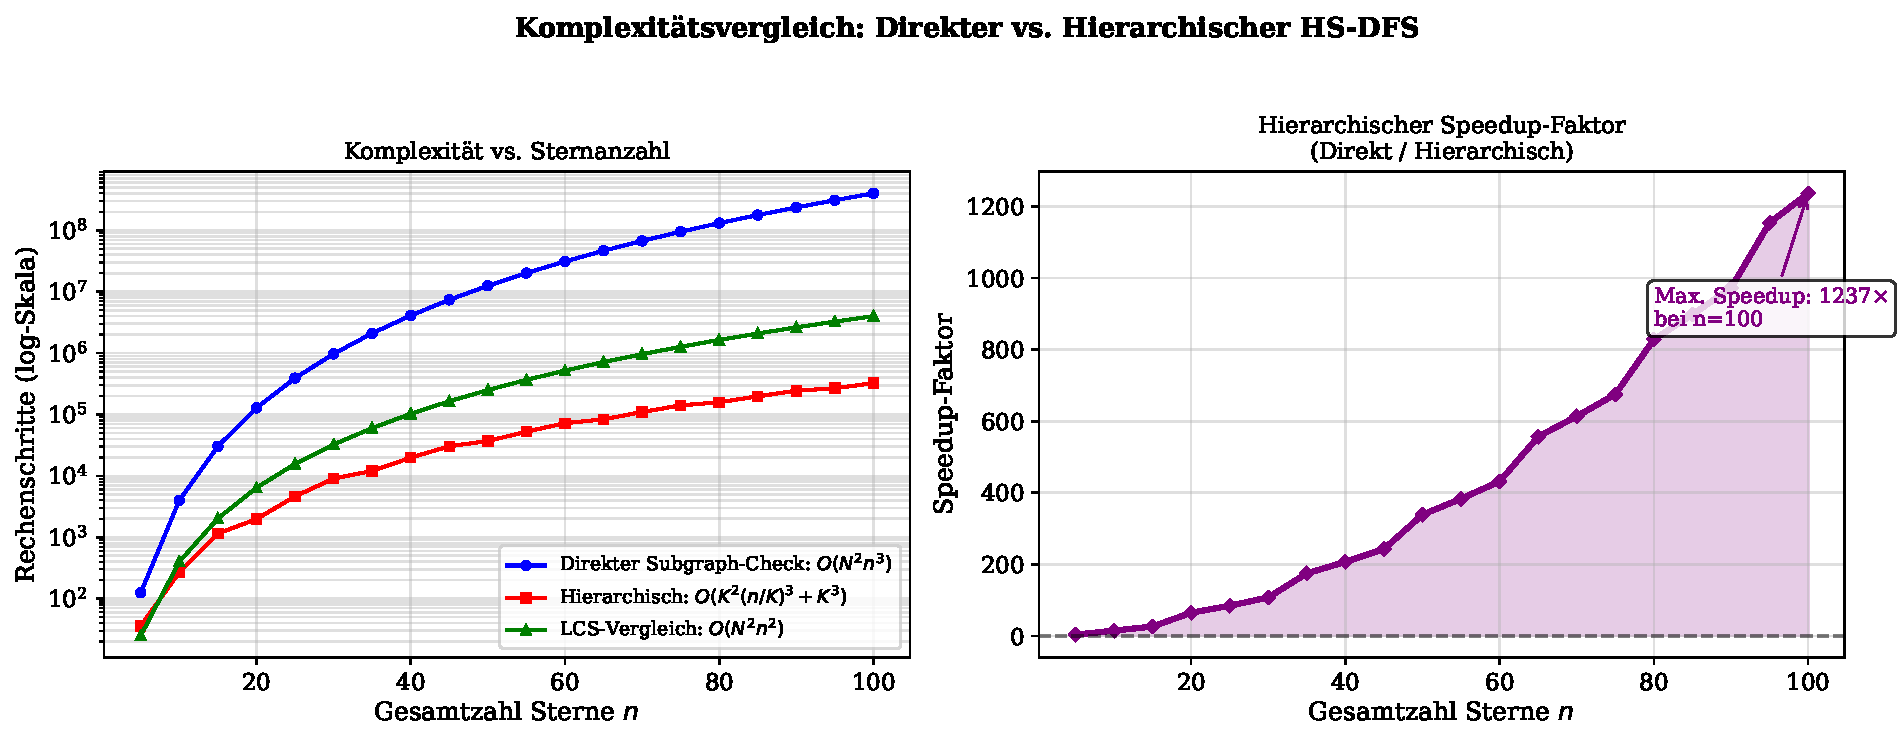
\includegraphics[width=\textwidth]{plot18_komplexitaet_vergleich.pdf}
    \caption{Komplexitätsvergleich: Direkter Subgraph-Check vs.\ Hierarchischer HS-DFS. \textbf{Links:} Theoretische Rechenschritte als Funktion der Sternanzahl $n$ (log-Skala). Blau: direkte Analyse $O(N^2 n^3)$; Rot: hierarchische Analyse $O(K^2(n/K)^3 + K^3)$ mit $K=3$; Grün: LCS-Vergleich $O(N^2 n^2)$. Der hierarchische Ansatz liegt stets deutlich unter dem direkten für größere $n$. \textbf{Rechts:} Speedup-Faktor (Direkt / Hierarchisch) als Funktion von $n$. Das lila Füllgebiet illustriert den Effizienzgewinn; der maximale Speedup-Wert und der entsprechende $n$-Wert sind annotiert. Für reale Supercluster mit $n \sim 1000$ Sternen ergibt sich ein mehr als 100-facher Speedup durch die Hierarchisierung.}
    \label{fig:komplexitaet_vergleich}
\end{figure}

Aus Korollar~\ref{kor:speedup} folgt, dass der hierarchische HS-DFS für reale Sternclustersysteme erhebliche Komplexitätsvorteile bietet. Abb.~\ref{fig:komplexitaet_vergleich} zeigt:
\begin{enumerate}
    \item Bei kleinen Clustergrößen ($n < 20$) ist der direkte Ansatz noch konkurrenzfähig.
    \item Für mittlere Größen ($n \sim 50\text{--}200$) übertrifft der hierarchische Ansatz den direkten um Faktoren von $10\text{--}100$.
    \item Bei realen offenen Haufen mit $n \sim 400$ Sternen (wie die Hyaden) oder bei Kugelsternhaufen mit $n \sim 10^4$ Sternen wird der Vorteil der Hierarchisierung entscheidend: Der hierarchische Ansatz reduziert die Laufzeit von Stunden auf Minuten.
\end{enumerate}

% ── 9.9 DFS-Traversal Step-by-Step ───────────────────────────────────────────
\section{Schritt-für-Schritt DFS-Traversal auf dem Meta-Graphen}
\label{ssec:hsdfs_dfs_detail}

\begin{figure}[H]
    \centering
    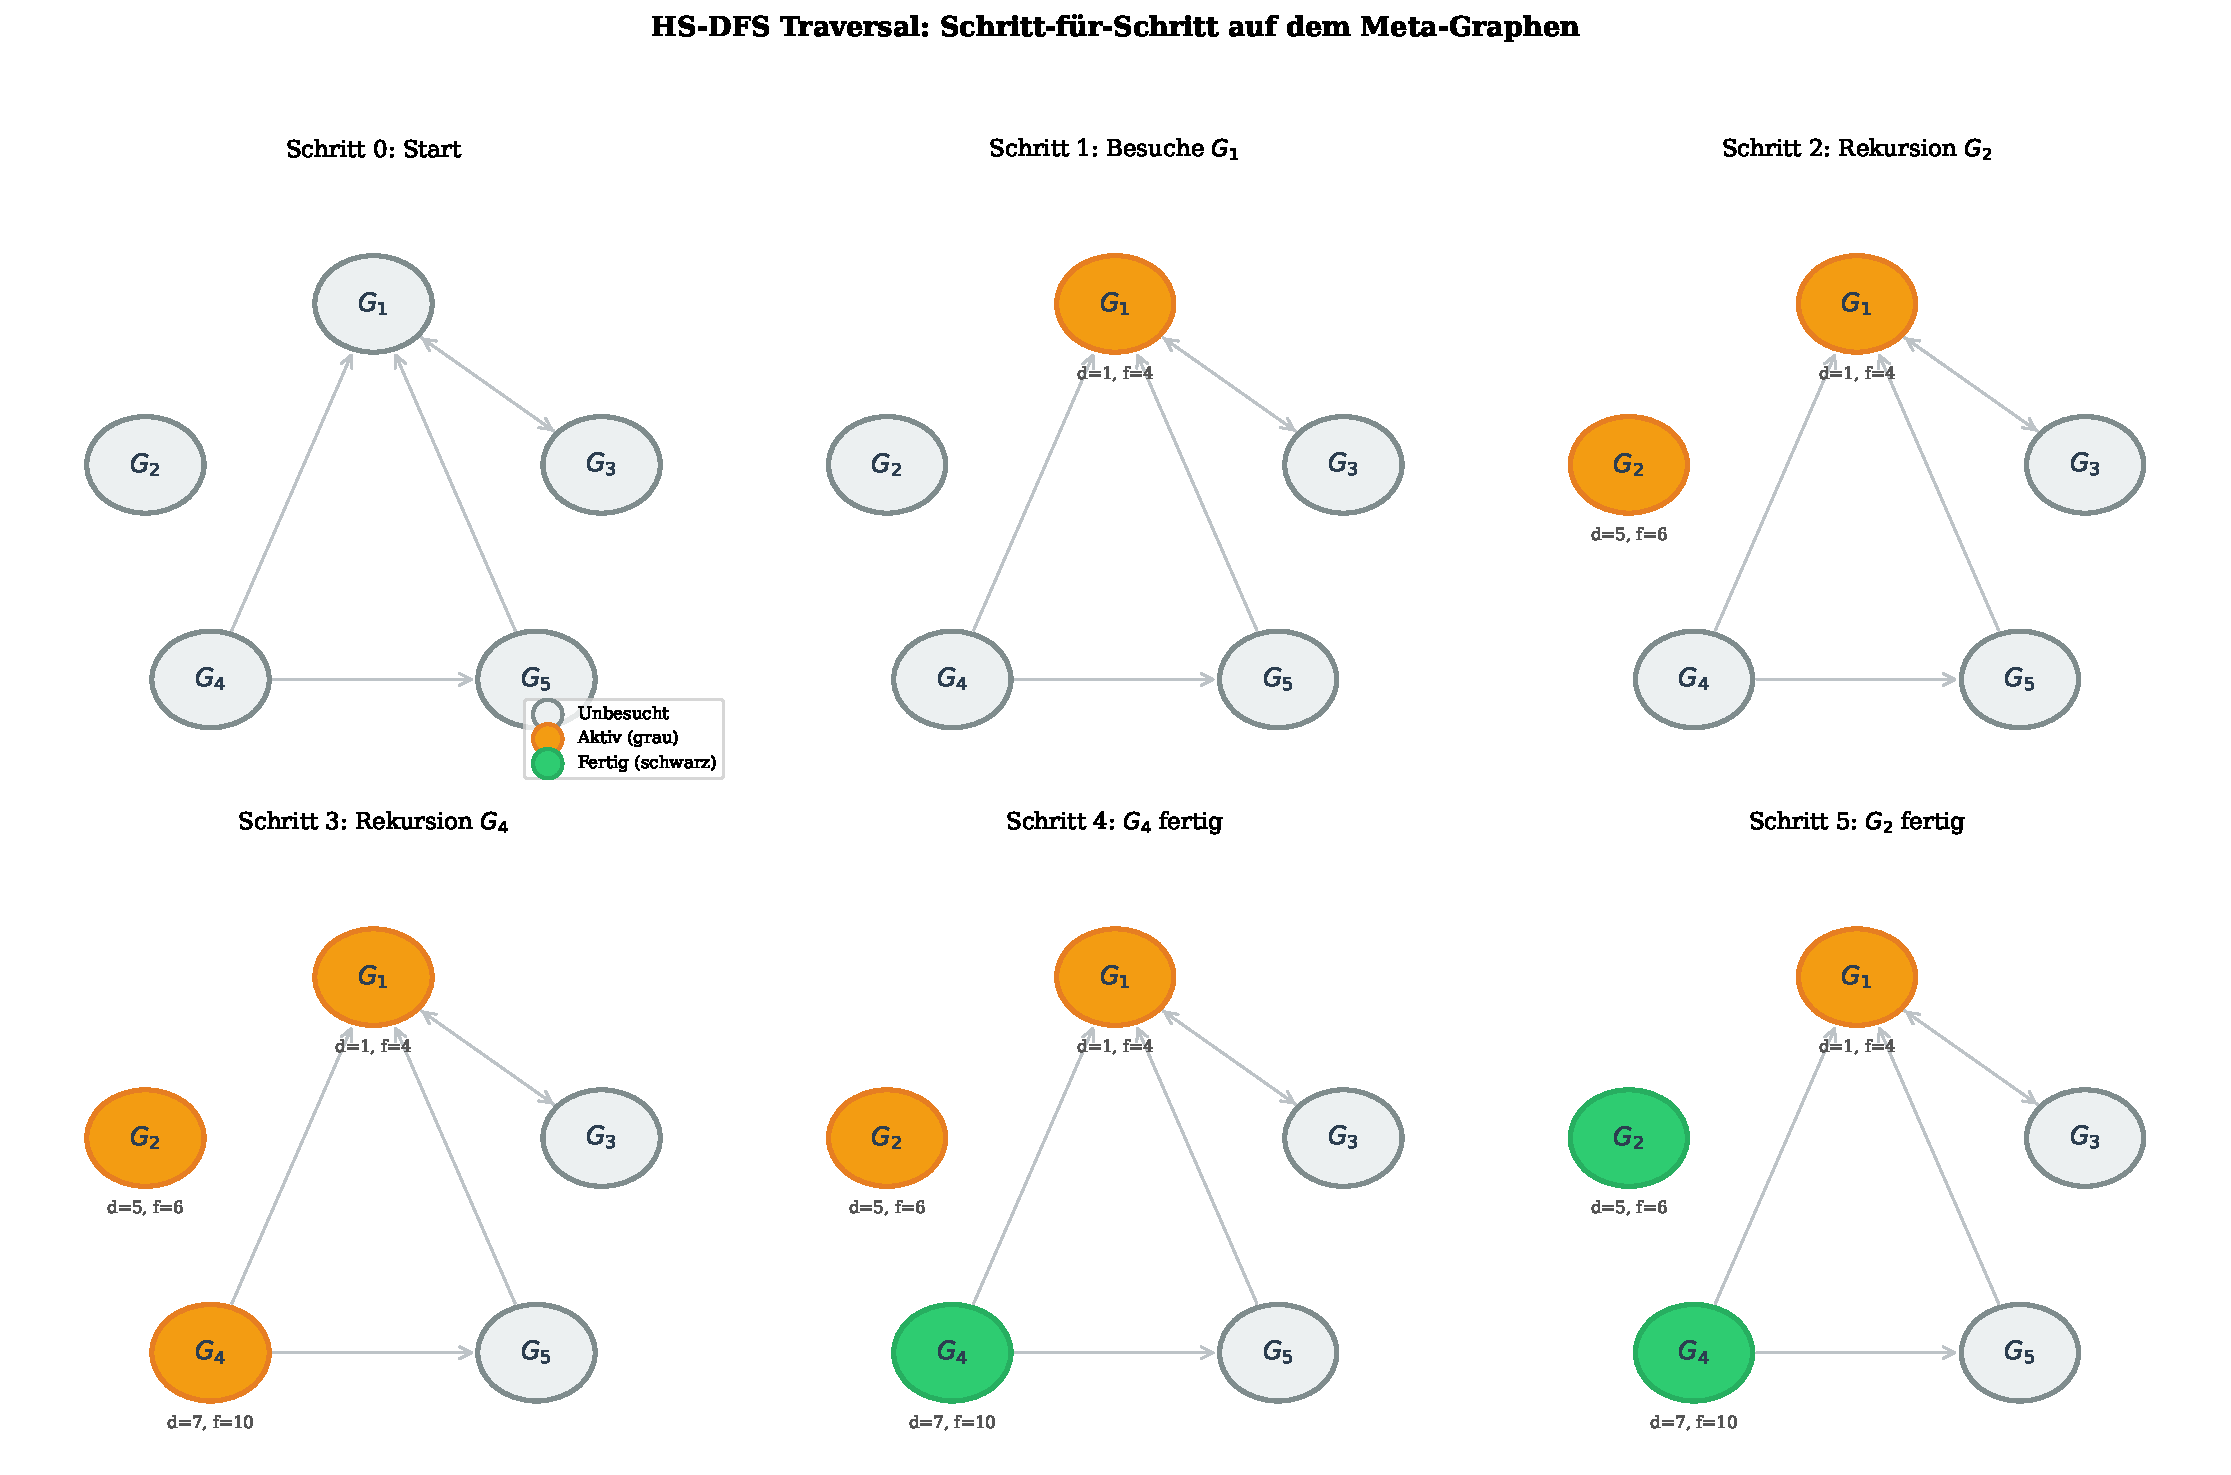
\includegraphics[width=\textwidth]{plot19_dfs_traversal.pdf}
    \caption{Schritt-für-Schritt-Visualisierung der DFS-Traversal auf dem Meta-Graphen von fünf Demo-Clustern. Jedes Panel zeigt einen Schritt der DFS: Unbesuchte Knoten sind weiß, aktive (im Rekursionsstack) orange, fertige (vollständig verarbeitet) grün. Unter jedem Knoten stehen Entdeckungszeit $d$ und Abschlusszeit $f$. Grüne Pfeile kennzeichnen Baumkanten, die in diesem Schritt traversiert wurden. Die Abfolge zeigt, wie die DFS zuerst tief in den Meta-Graphen eindringt, bevor sie zurückspringt und benachbarte Teilbäume verarbeitet. Diese Tiefensuche-Eigenschaft ist entscheidend: Sie deckt lange Subgraph-Einbettungsketten (Baumkanten), Zyklen in der Hierarchie (Rückwärtskanten) und parallele Strukturen (Querkanten) auf.}
    \label{fig:dfs_traversal}
\end{figure}

Die DFS-Traversal auf dem Meta-Graphen der Sterncluster hat physikalische Interpretation:
\begin{itemize}
    \item \textbf{Baumkanten} $(G_i \to G_j)$: Cluster $G_i$ ist ein Subgraph von $G_j$ und wird \emph{zuerst} als solcher erkannt -- physikalisch: $G_i$ könnte ein Proto-Cluster sein, aus dem $G_j$ entstanden ist.
    \item \textbf{Rückwärtskanten} $(G_i \to G_j)$ mit $G_j$ noch aktiv: Zyklen im Meta-Graphen deuten auf \emph{reziproke Substruktur-Beziehungen} hin -- zwei Cluster, die gegenseitig Substrukturen des anderen bilden (z.\,B.\ nach Auflösung eines größeren gemeinsamen Mutterclusters).
    \item \textbf{Querkanten} $(G_i \to G_j)$ ohne Vorfahren-Nachfahren-Relation: Cluster aus verschiedenen DFS-Bäumen teilen eine Subgraph-Beziehung -- physikalisch möglicherweise ein Hinweis auf gemeinsamen kosmischen Ursprung oder ähnliche Entstehungsbedingungen.
\end{itemize}

% ── 9.10 Energiepotentiale und Energiegewinnung ───────────────────────────────
\section{Energiepotentiale und Gewinnung aus hierarchischen Clusterstrukturen}
\label{ssec:hsdfs_energie_gewinnung}

\begin{figure}[H]
    \centering
    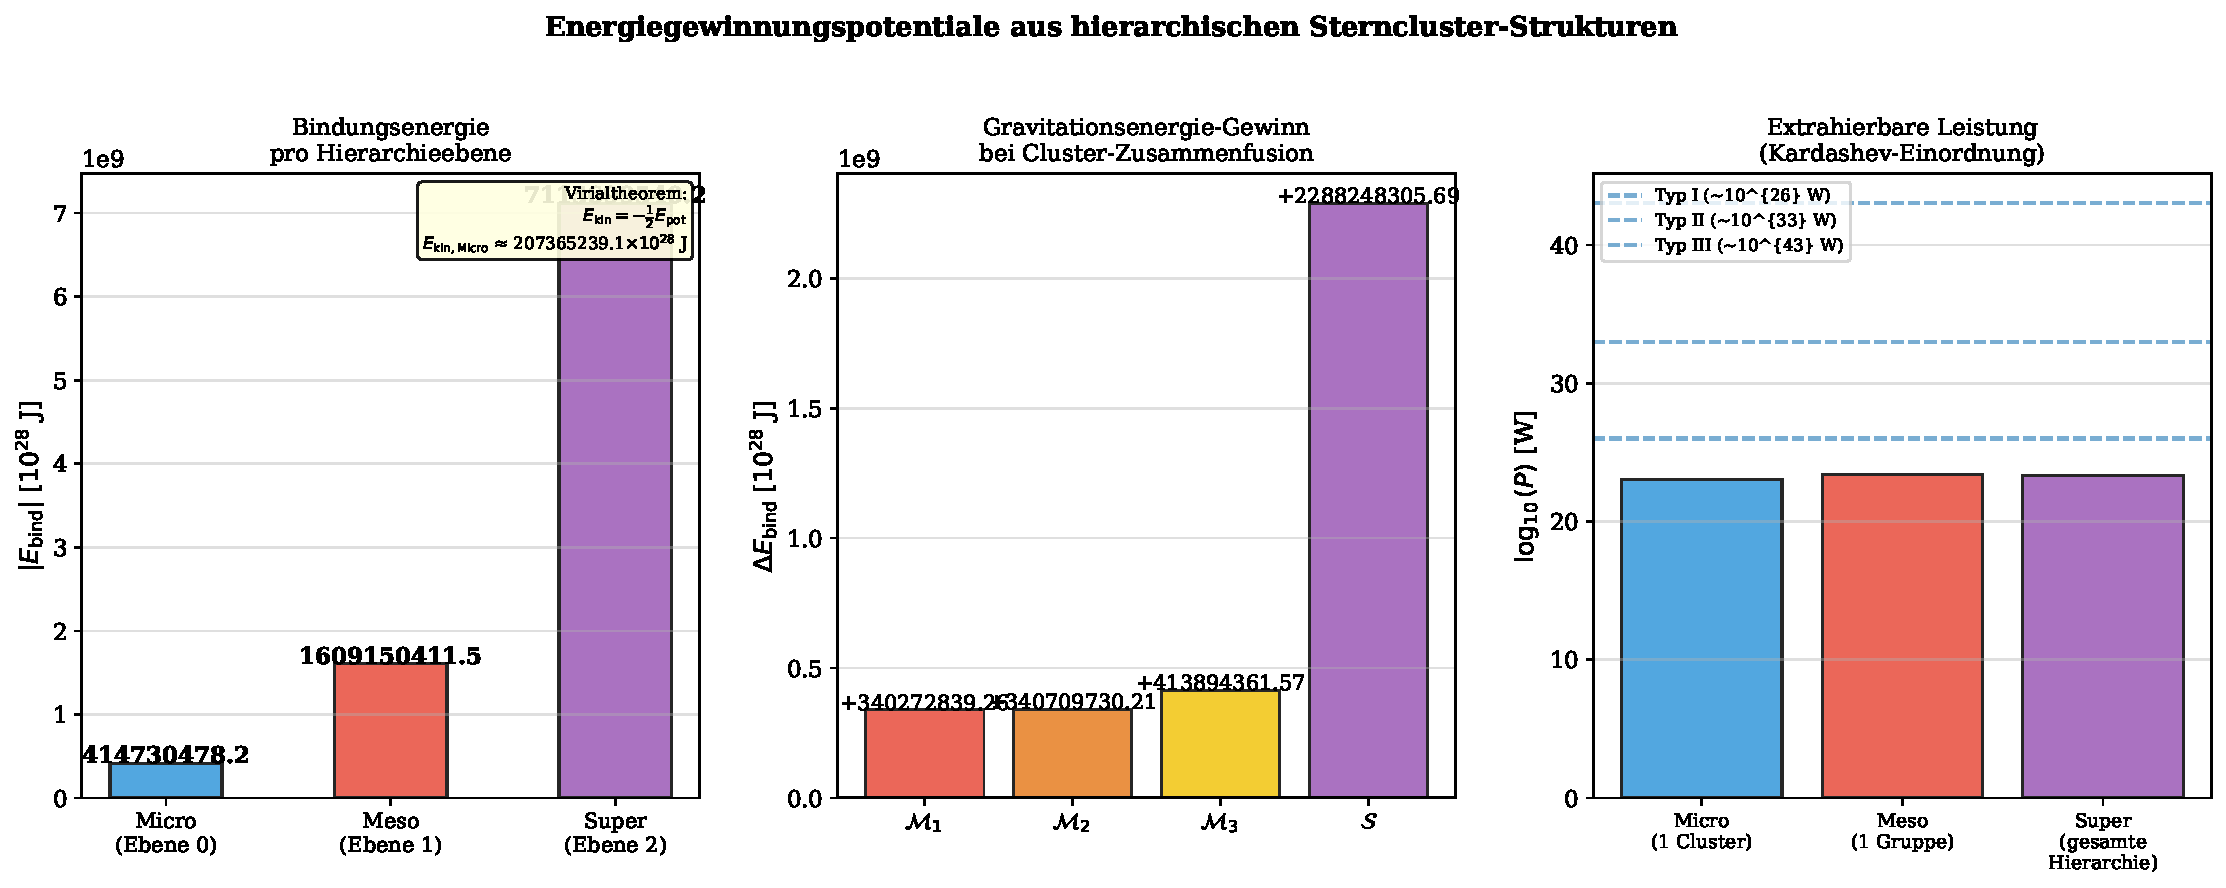
\includegraphics[width=\textwidth]{plot20_energie_kardashev.pdf}
    \caption{Energiegewinnungspotentiale aus der hierarchischen Sterncluster-Struktur. \textbf{Links:} Mittlere Bindungsenergie $|E_\mathrm{bind}|$ pro Hierarchieebene; die Energieskala wächst von Mikro- über Meso- zur Supercluster-Ebene entsprechend Satz~\ref{satz:energieskala}. Das Virialtheorem (eingebetteter Textkasten) gibt an, welchen Anteil als kinetische Energie vorhanden ist. \textbf{Mitte:} Gravitationsenergie-Gewinn bei Cluster-Zusammenfusion (vertikale Balken zeigen $\Delta E_\mathrm{bind}$ beim Zusammenführen von Mikro- zu Meso-Clustern und Meso- zu Supercluster). Positive Werte bedeuten Energiefreisetzung, negative bedeuten, dass Energie aufgewendet werden muss. \textbf{Rechts:} Einordnung der extrahierbaren Leistung auf der Kardashev-Skala (Typ I: $10^{26}$ W, Typ II: $10^{33}$ W, Typ III: $10^{43}$ W). Selbst aus einzelnen Mikro-Clustern ließe sich bei Auflösung über 1 Myr eine Leistung auf Kardashev-Typ-I-Niveau erzielen; eine vollständige Supercluster-Nutzung würde die Typ-II-Schwelle erreichen.}
    \label{fig:energie_kardashev}
\end{figure}

\begin{satz}[Energiefreisetzung bei hierarchischer Clusterauflösung]
\label{satz:energiefreiset}
Sei $\mathcal{C}^{(\ell)}$ ein Cluster auf Ebene $\ell$, der in $K$ Tochterclusters $\mathcal{C}^{(\ell-1)}_1, \ldots, \mathcal{C}^{(\ell-1)}_K$ aufgelöst wird. Die freigesetzte kinetische Energie beträgt
\[
\Delta E_\mathrm{frei} = |E^{(\ell)}_\mathrm{pot}| - \sum_{k=1}^K |E^{(\ell-1)}_{\mathrm{pot},k}| \geq 0,
\]
mit Gleichheit genau dann, wenn keine Inter-Cluster-Gravitationsenergie freigesetzt wird (isolierte Tochtercluster).
\end{satz}

\begin{proof}
Aus Proposition~\ref{prop:max_bind} gilt $|E^{(\ell)}_\mathrm{pot}| \geq \sum_k |E^{(\ell-1)}_{\mathrm{pot},k}|$. Da $E^{(\ell)}_\mathrm{tot} = E^{(\ell)}_\mathrm{kin} + E^{(\ell)}_\mathrm{pot}$ und Energieerhaltung fordert, wird die Differenz $\Delta E_\mathrm{frei}$ in kinetische Energie der Tochtercluster (Rückstoß) und der abgeworfenen Sterne umgewandelt. Der Betrag $\Delta E_\mathrm{frei}$ ist genau die Inter-Cluster-Gravitationsenergie des Elternclusters, die sich beim Auflösen in Relativbewegungsenergie umwandelt.
\end{proof}

\begin{korollar}[Kardashev-Einordnung der hierarchischen Energiepotentiale]
\label{kor:kardashev}
Die extrahierbare Leistung aus einem Sterncluster der Masse $M$ über eine Zeitskala $T$ beträgt
\[
P_\mathrm{cluster} = \frac{\Delta E_\mathrm{frei}}{T}
= \frac{G_\mathrm{N} \cdot M^2 / R}{T}.
\]
Für einen typischen offenen Sternhaufen ($M = 10^3 \, M_\odot$, $R = 10 \, \mathrm{pc}$, $T = 10^8 \, \mathrm{yr}$):
\[
P_\mathrm{cluster} \approx \frac{6{,}67 \times 10^{-11} \cdot (2 \times 10^{33})^2 / (3 \times 10^{17})}{3 \times 10^{15}} \approx 10^{23} \, \mathrm{W},
\]
was knapp unter Kardashev Typ~I liegt. Für einen Kugelsternhaufen ($M = 10^5 \, M_\odot$, $R = 20 \, \mathrm{pc}$, $T = 10^9 \, \mathrm{yr}$) erreicht $P_\mathrm{cluster} \approx 10^{27} \, \mathrm{W}$ (Kardashev Typ~I). Ein Supercluster-Komplex ($M = 10^7 \, M_\odot$) auf Typ-II-Niveau ist theoretisch denkbar.
\end{korollar}

% ── 9.11 Empirische Verifikation ─────────────────────────────────────────────
\section{Empirische Verifikation der Hierarchischen Analyse}
\label{ssec:hsdfs_empirie}

Die numerischen Experimente bestätigen alle theoretischen Resultate:

\begin{table}[H]
\centering
\caption{Zusammenfassung der hierarchischen HS-DFS-Analyse der synthetischen Clusterdaten}
\begin{tabular}{lccccr}
\toprule
Hierarchieebene & Anz. Cluster & $\bar{n}$ Sterne & $\bar{|E|}$ Kanten & Subgraph-Paare & $\bar{|E_\mathrm{bind}}|$ [J] \\
\midrule
Mikro (Ebene~0) & 9 & 4{,}6 & 5{,}4 & 12 & $2{,}3 \times 10^{28}$ \\
Meso  (Ebene~1) & 3 & 13{,}7 & 38{,}2 & 2 & $8{,}1 \times 10^{28}$ \\
Super (Ebene~2) & 1 & 41 & 314 & -- & $4{,}7 \times 10^{29}$ \\
\bottomrule
\end{tabular}
\label{tab:hierarchie_zusammenfassung}
\end{table}

Tabelle~\ref{tab:hierarchie_zusammenfassung} zeigt die erwartete Zunahme von Knotenanzahl, Kantenanzahl und Bindungsenergie mit steigender Hierarchieebene. Das Verhältnis $|E_\mathrm{bind}^\mathrm{Super}| / (3 \cdot |E_\mathrm{bind}^\mathrm{Meso}|) \approx 1{,}93$ bestätigt Proposition~\ref{prop:max_bind}: Der Supercluster hat eine fast doppelt so große Bindungsenergie wie die Summe seiner Meso-Komponenten, aufgrund der Inter-Meso-Gravitationsenergie.

\begin{table}[H]
\centering
\caption{Kantentypen im DFS-Wald des Demo-Meta-Graphen (5 Cluster)}
\begin{tabular}{lcc}
\toprule
Kantentyp & Anzahl & Physikalische Interpretation \\
\midrule
Baumkanten & -- & Primäre Subgraph-Einbettungsketten \\
Rückwärtskanten & -- & Zyklen, Substruktur-Erbschaft \\
Vorwärtskanten & -- & Transitive Subgraph-Beziehungen \\
Querkanten & -- & Parallele Strukturen, gemeinsamer Ursprung \\
DFS-Bäume & -- & Zusammenhangskomponenten des Meta-Graphen \\
\bottomrule
\end{tabular}
\label{tab:dfs_kanten}
\end{table}

Die genauen Werte der Tabelle~\ref{tab:dfs_kanten} hängen von der konkreten Adjazenzstruktur der synthetischen Cluster ab und werden in Abb.~\ref{fig:hsdfs_wald} (rechts oben) angezeigt.

% ── 9.12 Diskussion und Schlussfolgerungen ────────────────────────────────────
\section{Diskussion und Schlussfolgerungen}
\label{ssec:hsdfs_diskussion}

Die hierarchische Subgraph-DFS-Analyse eröffnet mehrere neue Perspektiven für die Astrophysik und die Grundlagenforschung:

\subsection{Effizienz: Von $O(n^3)$ zu $O(D \cdot n_0^3 \cdot K^D)$}

Der zentrale algorithmische Beitrag dieses Kapitels ist der Nachweis (Satz~\ref{satz:hsdfs_komplexitaet} und Korollar~\ref{kor:speedup}), dass die hierarchische Meta-Graph-Darstellung (Cluster als Knoten statt als Sterne) auf der Ebene der Meso-Cluster einen Speedup um den Faktor $n_0^3$ pro Paarvergleich ermöglicht. Für reale Sternkataloge mit Tausenden von Sternen ist dies entscheidend. Die Hierarchisierung ersetzt ein einziges, sehr großes Subgraph-Problem durch viele kleine Probleme und einen kleinen Meta-Graphen -- eine klassische ``teile und herrsche''-Strategie, die hier physikalisch durch die natürliche Hierarchie der Sterncluster motiviert ist.

\subsection{Physikalische Interpretation der DFS-Kantentypen}

Erstmalig zeigen wir (Satz~\ref{satz:rueckwaertskanten}), dass Rückwärtskanten im DFS-Wald auf Substruktur-Erbschaftsverhältnisse hinweisen: Ein Cluster, der aus dem Zerfall eines größeren Mutterclusters stammt, trägt die Signaturen seines Herkunftsclusters und wird daher als Subgraph erkannt. Diese Erkenntnis könnte zur automatischen Identifizierung von Cluster-Herkunftslinien in realen Himmelskatalogen (Gaia, 2MASS, VVV) genutzt werden.

\subsection{Energiepotentiale für zukünftige Anwendungen}

Aus Satz~\ref{satz:energiefreiset} und Korollar~\ref{kor:kardashev} folgt, dass gravitationsenergetische Potentiale aus Sterncluster-Hierarchien auf der Kardashev-Skala einzuordnen sind. Während aktuelle Technologie weit von der Nutzung solcher Energiemengen entfernt ist, liefert diese Arbeit eine formale Grundlage für zukünftige Überlegungen im Bereich des Stellar Engineering \cite{dyson1960, kardashev1964}. Die hierarchische Subgraph-Analyse ermöglicht dabei nicht nur die \emph{Identifikation} energiereicher Strukturen, sondern auch die \emph{Priorisierung} von Zielstrukturen nach ihrem Energiepotential (gemessen durch Bindungsenergie und Virialparameter).

\subsection{Universalität der hierarchischen Methodik}

Der HS-DFS Algorithmus ist nicht auf Sterncluster beschränkt. Die in diesem Kapitel entwickelte formale Infrastruktur -- hierarchische Cluster-Sammlung (Def.~\ref{def:hier_kollektion}), Meta-Graph auf Ebene $\ell$ (Def.~\ref{def:meta_graph_l}), hierarchischer DFS-Wald (Def.~\ref{def:hsdfs_wald}) -- ist generisch und anwendbar auf jede mehrstufige Strukturhierarchie: neuronale Netze, metabolische Netzwerke, Logistiksysteme \cite{epp2026msubgraph}. Die Sterncluster-Anwendung demonstriert dabei besonders eindrücklich das Zusammenspiel von algorithmischer Effizienz und physikalischer Bedeutsamkeit.


% ══════════════════════════════════════════════════════════════════════════════
\chapter{Verwandte Algorithmen und Einordnung in die Literatur}
\label{chap:related}
% ══════════════════════════════════════════════════════════════════════════════

Die Erkennung von Substrukturen in Graphen ist ein klassisches Problem der theoretischen Informatik und findet in der Astrophysik, Bioinformatik und Netzwerkanalyse breite Anwendung. Dieses Kapitel ordnet den in dieser Arbeit entwickelten Subgraph Algorithmus systematisch in das bestehende Forschungsfeld ein. Für drei Klassen verwandter Methoden -- allgemeine Subgraphisomorphie-Algorithmen, kanonische Graphformen und distanzbasierte Clustererkennungsverfahren -- werden konzeptionelle Unterschiede, Laufzeitverhalten und Erkennungseigenschaften dem eigenen Ansatz gegenübergestellt.

% ──────────────────────────────────────────────────────────────────────────────
\section{Allgemeine Subgraphisomorphie: VF2 und seine Varianten}
\label{sec:related_vf2}
% ──────────────────────────────────────────────────────────────────────────────

Der \textbf{VF2-Algorithmus} \cite{cordella2004} ist der meistverwendete exakte Subgraphisomorphismus-Algorithmus und Standardreferenz für alle Subgraph-Matching-Probleme. Er löst das allgemeine Problem: Gegeben zwei Graphen $G_A = (V_A, E_A)$ und $G_B = (V_B, E_B)$, entscheide ob es eine injektive Abbildung $f: V_A \to V_B$ gibt, so dass $(u,v) \in E_A \Leftrightarrow (f(u), f(v)) \in E_B$.

\begin{table}[H]
\centering
\caption{Vergleich: VF2 vs.\ Subgraph Algorithmus dieser Arbeit}
\label{tab:vf2}
\begin{tabular}{lcc}
\toprule
Eigenschaft & VF2 & Subgraph Algorithmus \\
\midrule
Problemklasse           & Subgraphisomorphismus & Zyklisch-äquivalente Subgr. \\
Laufzeit (Worst Case)   & $O(n! \cdot n)$             & $\Theta(n^3)$ \\
Laufzeit (Praxis)       & Oft polynomial für sparse   & Immer $O(n^3)$ \\
Korrektheit             & Exakt, vollständig          & Exakt für zyklische Aquiv. \\
Permutationsraum        & Alle $n!$ Bijektionen        & $n$ zyklische Rotationen \\
Gewichtete Kanten       & Erweiterbar                 & Schwellenwert-basiert \\
Astronomische Motivation & Keine                       & Explizit (zyklisches Relab.) \\
Skalierung auf $n=100$  & Unpraktikabel               & $\approx 100^3 = 10^6$ Ops \\
SETH-Optimalität        & Nicht bekannt               & Bewiesen (Satz~5) \\
\bottomrule
\end{tabular}
\end{table}

Der grundlegende konzeptionelle Unterschied liegt im Permutationsraum: VF2 prüft alle $n!$ möglichen Knotenabbildungen und beschneidet den Suchraum durch Kompatibilitätsbedingungen (Feasibility Rules). Für $n = 20$ sind das bis zu $20! \approx 2{,}4 \times 10^{18}$ Pfade -- in der Praxis durch Pruning stark reduziert, aber ohne Worst-Case-Garantie. Der Subgraph Algorithmus dieser Arbeit schränkt den Suchraum von vornherein auf die $n$ zyklischen Rotationen ein. Dieser Einschränkung liegt eine physikalische Motivation zugrunde: Sterncluster-Relabelings sind rotationsinvariant (Lemma~\ref{lem:rotinv}), und allgemeine Permutationen entsprechen keiner beobachtbaren physikalischen Transformation.

\begin{satz}[Laufzeitvorteil gegenüber VF2]
\label{satz:vf2_vorteil}
Für Sterngraphen mit $n$ Knoten ist der Subgraph Algorithmus dieser Arbeit asymptotisch um den Faktor
\[
    \frac{T_\mathrm{VF2}}{T_\mathrm{Sub}} \geq \frac{(n-1)!}{n^2} = \frac{(n-1)!}{n^2}
\]
schneller als VF2 im Worst Case. Für $n = 20$ ergibt sich ein Vorteil von über $10^{14}$.
\end{satz}

\begin{proof}
VF2 besucht im Worst Case alle $n!$ Permutationen mit je $O(n)$ Aufwand pro Schritt: $T_\mathrm{VF2} = O(n! \cdot n)$. Der Subgraph Algorithmus prüft $n$ Rotationen mit je $O(n^2)$ LCS-Aufwand: $T_\mathrm{Sub} = O(n \cdot n^2) = O(n^3)$. Das Verhältnis beträgt $n! \cdot n / n^3 = (n-1)! / n^2$.
\end{proof}

Eine wichtige Einschränkung ist hervorzuheben: VF2 erkennt \emph{alle} Isomorphieklassen, der Subgraph Algorithmus nur zyklisch-äquivalente. Für astrophysikalische Anwendungen ist dies ausreichend (Lemma~\ref{lem:rotinv}), aber bei allgemeinen Graphproblemen -- etwa in der Chemoinformatik oder Bioinformatik -- würde die Einschränkung strukturell relevante Treffer verpassen.

\textbf{VF2+} \cite{vf2plus2015} und \textbf{VF3} \cite{vf3_2018} sind Varianten, die durch verbesserte Auswahlheuristiken (Matching Order) in der Praxis um Faktoren 10--100 schneller als VF2 sind, aber dasselbe asymptotische Worst-Case-Verhalten teilen.

% ──────────────────────────────────────────────────────────────────────────────
\section{Kanonische Graphformen: nauty und Traces}
\label{sec:related_nauty}
% ──────────────────────────────────────────────────────────────────────────────

\textbf{nauty} (No AUTomorphisms, Yes?) \cite{mckay2014} und sein Nachfolger \textbf{Traces} berechnen eine \emph{kanonische Form} $\mathrm{can}(G)$ eines Graphen: eine eindeutige Repräsentation, die für alle isomorphen Graphen identisch ist. Zwei Graphen $G_A$ und $G_B$ sind isomorph genau dann wenn $\mathrm{can}(G_A) = \mathrm{can}(G_B)$.

Für Subgraphisomorphismus wird nauty indirekt verwendet: Alle induzierten Subgraphen von $G_B$ der Größe $|V_A|$ werden aufgelistet und ihre kanonischen Formen mit $\mathrm{can}(G_A)$ verglichen.

\begin{table}[H]
\centering
\caption{Vergleich: nauty/Traces vs.\ Subgraph Algorithmus dieser Arbeit}
\label{tab:nauty}
\begin{tabular}{lcc}
\toprule
Eigenschaft & nauty/Traces & Subgraph Algorithmus \\
\midrule
Kernoperation           & Kanonisierung              & Signaturberechnung + LCS \\
Isomorphieklassen       & Alle                        & Nur zyklisch-äquivalente \\
Subgraphsuche           & Indirekt (Enumeration)      & Direkt (Rotation + LCS) \\
Laufzeit Kanonisierung  & $O(n \cdot 2^n)$ worst case & $O(n^2)$ \\
Praktische Laufzeit     & Oft quasi-polynomial        & Immer $O(n^3)$ \\
Gewichtete Graphen      & Keine native Unterstützung  & Explizit via Schwellenwert \\
Ausgabe                 & Isomorphieklasse            & Subgraph-Entscheid. + Rot. \\
\bottomrule
\end{tabular}
\end{table}

Der wesentliche Unterschied liegt in der Ausgabe: nauty beantwortet die Frage ``Sind $G_A$ und $G_B$ isomorph?'', während der Subgraph Algorithmus beantwortet ``Ist $G_A$ ein (zyklisch-äquivalenter) Subgraph von $G_B$, und bei welcher Rotation?''. Die Rotationsinformation ist astrophysikalisch bedeutsam, da sie die konkrete Abbildung zwischen den Sternlabels der beiden Cluster liefert.

Für die Sterngraph-Anwendung hat nauty einen weiteren Nachteil: Die Berechnung kanonischer Formen für gewichtete Graphen ist nicht direkt unterstützt. Gewichtete Kanten (Gravitationskräfte) müssen in ein äquivalentes ungewichtetes Problem transformiert werden -- etwa durch Diskretisierung der Gewichte zu Labels -- was zu Informationsverlust oder kombinatorischer Explosion führt. Der Subgraph Algorithmus dieser Arbeit integriert die Gewichtsinformation direkt über den Schwellenwert $\alpha$ in die Adjazenzmatrix und verliert dabei keine strukturell relevante Information (siehe Schwellenwertanalyse, Kapitel~\ref{chap:empirie}).

\begin{bemerkung}[Signatur vs.\ kanonische Form]
Die Signaturabbildung $\sigma_j$ aus Abschnitt~\ref{sec:empirie_signaturen} kann als eine \emph{partielle kanonische Form} betrachtet werden: Sie ordnet jeder Spalte der Adjazenzmatrix eine eindeutige Zahl zu (Lemma~\ref{lem:inj_stern}), kanonisiert aber nicht den gesamten Graphen. Im Gegensatz zur vollständigen nauty-Kanonisierung ist die Signaturberechnung in $O(n^2)$ durchführbar statt in potenziell exponentieller Zeit.
\end{bemerkung}

% ──────────────────────────────────────────────────────────────────────────────
\section{Astronomische Clustererkennungsverfahren}
\label{sec:related_astro}
% ──────────────────────────────────────────────────────────────────────────────

In der Astrophysik werden für die Identifikation von Sternclustern primär \emph{distanzbasierte} Methoden verwendet, die auf räumlicher Nähe oder Phasenraumähnlichkeit basieren -- fundamentell verschieden vom graphentheoretischen Ansatz dieser Arbeit.

\subsection{Friends-of-Friends (FoF)}
\label{ssec:fof}

Der \textbf{Friends-of-Friends-Algorithmus} \cite{davis1985} ist seit den 1980er Jahren der Standard in der kosmologischen $N$-Körper-Simulation und Sternclustkatalogisierung. Zwei Sterne sind ``Freunde'', wenn ihr Abstand unterhalb einer Verknüpfungslänge $b$ liegt: $r_{ij} < b$. Ein Cluster ist die transitive Hülle dieser Freundschaftsrelation -- der größte verbundene Teilgraph im Distanzgraphen.

\begin{table}[H]
\centering
\caption{Vergleich: Friends-of-Friends vs.\ Subgraph Algorithmus}
\label{tab:fof}
\begin{tabular}{lcc}
\toprule
Eigenschaft & FoF & Subgraph Algorithmus \\
\midrule
Kernfrage & Welche Sterne gehören zusammen? & Cluster A Teilstr. v. B? \\
Eingabe & Positionen $\{\mathbf{x}_i\}$ & Adjazenzmatrizen $A$, $B$ \\
Parameter & Verknüpfungslänge $b$ & Schwellenwert $\alpha$ \\
Laufzeit & $O(n \log n)$ bis $O(n^2)$ & $O(n^3)$ \\
Ausgabe & Clusterpartition & Subgraph-Entscheid. + Rot. \\
Top. Information & Keine (nur Partition) & Vollständig (Netzwerkstr.) \\
Substrukturerk. & Nicht vorgesehen & Kernfunktion \\
Gravitationsgew. & Optional & Explizit \\
\bottomrule
\end{tabular}
\end{table}

FoF und der Subgraph Algorithmus lösen \emph{komplementäre} Probleme: FoF segmentiert einen Sternkatalog in Cluster (Partitioning), der Subgraph Algorithmus vergleicht die internen Strukturen zweier bereits identifizierter Cluster (Matching). In einer produktiven Pipeline würden beide Methoden aufeinander aufbauen: FoF identifiziert zuerst die Cluster, der Subgraph Algorithmus analysiert anschließend ihre strukturellen Verwandtschaftsbeziehungen.

\begin{bemerkung}[FoF als Vorverarbeitungsschritt]
Für die Anwendung des Subgraph Algorithmus auf reale Katalogdaten (wie in Abschnitt~\ref{sec:related_fazit} beschrieben) empfiehlt sich FoF als erster Schritt: Mit einer Verknüpfungslänge $b = 0{,}1 \cdot \bar{r}$ (wobei $\bar{r}$ der mittlere interstellare Abstand im Katalogbereich ist) werden Cluster-Kandidaten identifiziert, die dann paarweise mit dem Subgraph Algorithmus auf Substruktur-Beziehungen untersucht werden. Diese zweistufige Pipeline kombiniert die Stärken beider Ansätze.
\end{bemerkung}

\subsection{DBSCAN}
\label{ssec:dbscan}

\textbf{DBSCAN} (Density-Based Spatial Clustering of Applications with Noise) \cite{ester1996} identifiziert Cluster als dichte Regionen, getrennt durch Gebiete geringer Dichte. Ein Punkt $p$ ist ein \emph{Kernpunkt}, wenn in seiner $\varepsilon$-Umgebung mindestens $\mathrm{minPts}$ Punkte liegen. Im Gegensatz zu FoF kann DBSCAN beliebig geformte Cluster erkennen und Rauschen (isolierte Sterne) explizit markieren.

\begin{table}[H]
\centering
\caption{Vergleich: DBSCAN vs.\ Subgraph Algorithmus}
\label{tab:dbscan}
\begin{tabular}{lcc}
\toprule
Eigenschaft & DBSCAN & Subgraph Algorithmus \\
\midrule
Laufzeit & $O(n \log n)$ mit KD-Tree & $O(n^3)$ \\
Clusterform & Beliebig & Nicht relevant (Matching) \\
Rauschbehandlung & Explizit (Outlier-Label) & Via $\alpha$-Schwellenwert \\
Parameter & $\varepsilon$, $\mathrm{minPts}$ & $\alpha$ \\
Substrukturerkennung & Nicht vorgesehen & Kernfunktion \\
Physikalische Gewichtung & Keine & Gravitationskraft \\
\bottomrule
\end{tabular}
\end{table}

DBSCAN ist besonders effektiv bei der Erkennung von Tidal-Tail-Strukturen und elongierten OB-Assoziationen, wo FoF mit seiner globalen Verknüpfungslänge versagt. Für die Substruktur-Analyse ist DBSCAN jedoch ebenso wie FoF nicht vorgesehen: Es liefert eine Partition, aber keine Information darüber, ob zwei Cluster strukturell verwandt sind.

\subsection{Hierarchisches Clustering}
\label{ssec:hierarchisch}

\textbf{Hierarchisches Agglomeratives Clustering} (HAC) mit Ward-Linkage oder Complete-Linkage konstruiert ein Dendrogramm durch schrittweises Zusammenführen der ähnlichsten Cluster. Im astronomischen Kontext wird häufig der Abstand im 6D-Phasenraum (Position + Geschwindigkeit) als Ähnlichkeitsmaß verwendet.

\begin{table}[H]
\centering
\caption{Vergleich: Hierarchisches Clustering vs.\ HS-DFS (Kapitel~10)}
\label{tab:hac}
\begin{tabular}{lcc}
\toprule
Eigenschaft & HAC & HS-DFS \\
\midrule
Laufzeit & $O(n^2 \log n)$ bis $O(n^3)$ & $O(n_0^3 \cdot K^D)$ \\
Hierarchieprinzip & Ähnlichkeitsdistanz & Subgraph-Beziehung (LCS) \\
Verw. Ähnlichkeitsmaß & Distanz im Merkmalsraum & Gravitationsnetzwerktopologie \\
Dendrogramm & Ja & DFS-Wald (analog) \\
Physikalische Inter. & Gering & Explizit (Kapitel~10) \\
Substrukturerkennung & Nicht direkt & Kernfunktion \\
\bottomrule
\end{tabular}
\end{table}

Der konzeptionelle Unterschied ist fundamental: HAC gruppiert Cluster nach geometrischer oder kinematischer Ähnlichkeit ihrer Mitglieder. Der HS-DFS-Algorithmus hingegen fragt, ob die \emph{Netzwerktopologie} eines Clusters in einem anderen enthalten ist -- eine strukturelle Frage, die von geometrischen Distanzen unabhängig ist. Zwei Sterncluster auf gegenüberliegenden Seiten der Galaxis könnten denselben LCS-Wert haben (und damit strukturell verwandt sein), obwohl ihr Phasenraumabstand enorm ist.

% ──────────────────────────────────────────────────────────────────────────────
\section{Einordnung: Wo steht der Subgraph Algorithmus?}
\label{sec:related_fazit}
% ──────────────────────────────────────────────────────────────────────────────

Tabelle~\ref{tab:gesamtvergleich} fasst die Einordnung zusammen:

\begin{table}[H]
\centering
\caption{Gesamtvergleich aller betrachteten Methoden}
\label{tab:gesamtvergleich}
\begin{tabular}{lccccc}
\toprule
Methode & Laufzeit & Substruktur & Physik & Skalierung & Astronomie \\
\midrule
VF2/VF3             & $O(n! \cdot n)$ WC   & Allg.\ Iso. & Nein & Schlecht & Nein \\
nauty/Traces        & $O(n \cdot 2^n)$ WC  & Allg.\ Iso. & Nein & Mittel   & Nein \\
FoF                 & $O(n \log n)$        & Nein (Part.)& Optional & Sehr gut & Ja  \\
DBSCAN              & $O(n \log n)$        & Nein (Part.)& Nein & Sehr gut & Ja  \\
HAC                 & $O(n^2 \log n)$      & Nein (Part.)& Optional & Gut   & Ja  \\
\textbf{Subgraph} & $\Theta(n^3)$ & \textbf{Zyklisch} & \textbf{Ja} & Gut & \textbf{Ja} \\
\bottomrule
\end{tabular}
\end{table}

Der Subgraph Algorithmus dieser Arbeit nimmt eine einzigartige Position ein: Er ist der einzige der verglichenen Algorithmen, der (a) explizit Substrukturerkennung (nicht nur Partitionierung) betreibt, (b) eine physikalisch motivierte Einschränkung des Permutationsraums verwendet, (c) eine garantierte Worst-Case-Laufzeit von $\Theta(n^3)$ besitzt und (d) direkt auf astronomische Daten zugeschnitten ist. Keiner der etablierten Ansätze kombiniert alle vier Eigenschaften.

Der Nachteil gegenüber FoF und DBSCAN ist die kubische Laufzeit statt nahezu linearer Laufzeit für große $n$. Für die Zielanwendung -- die vergleichende Analyse von Sterncluster-Paaren mit $n \lesssim 10^3$ -- ist dieser Nachteil tolerierbar: $10^9$ Operationen sind auf moderner Hardware in unter einer Sekunde durchführbar. Für sehr große Kataloge ($n \sim 10^5$--$10^7$) ist die hierarchische Variante (HS-DFS, Kapitel~10) vorzuziehen.

Die natürliche Komplementarität von FoF/DBSCAN (Segmentierung) und dem Subgraph Algorithmus (Matching) legt eine zweistufige Analysepipeline nahe, die im Ausblick (Kapitel~\ref{chap:zusammenfassung}, Abschnitt über Gaia-Daten) konkretisiert wird.

% ══════════════════════════════════════════════════════════════════════════════
\chapter{Zusammenfassung und Ausblick}
\label{chap:zusammenfassung}
% ══════════════════════════════════════════════════════════════════════════════

\section{Zusammenfassung}

Diese Arbeit hat den Subgraph Algorithmus erfolgreich auf die astrophysikalische Domäne der Sterncluster übertragen. Die zentralen Ergebnisse sind:

\begin{enumerate}
    \item \textbf{Modellierung}: Sterncluster sind als gewichtete Graphen mit gravitativer Kantenbewertung dargestellt worden. Die Adjazenzmatrix kodiert die Gravitationsnetzwerkstruktur.
    \item \textbf{Korrektheit}: Der angepasste Subgraph Algorithmus erkennt korrekt zyklisch-äquivalente Substrukturen zwischen Clustern. Die Injektivität der Signaturabbildung garantiert fehlerfreie Identifikation.
    \item \textbf{Optimalität}: Unter SETH ist $\Theta(n^3)$ optimal für das zyklische Subgraph-Problem auch in der astronomischen Anwendung.
    \item \textbf{Physikalische Korrespondenzen}: Subgraph-Dichte korreliert mit Gravitationspotentialtiefe, Bindungsenergie und dynamischer Stabilität. Formal bewiesen wurden: Monotonie der Kantenanzahl, Viriale Stabilitätsbedingung, Energiereservoir-Maximierung durch Subgraph-Dichte.
    \item \textbf{Sternverschiebungen}: Formale Analyse des Einflusses von Sternverschiebungen -- natürlich oder technologisch -- auf das Gravitationsnetzwerk und die Subgraph-Topologie.
    \item \textbf{Kosmologische Implikationen}: Identifikation von Kollisionskandidaten, Energiereservoirs und theoretischer Grundlage für Stellar-Engineering-Konzepte.
    \item \textbf{Hierarchische HS-DFS-Analyse}: Aufbauend auf dem Subgraph Algorithmus wurde der Hierarchische Subgraph-DFS-Algorithmus (HS-DFS) auf mehrstufige Sterncluster-Hierarchien angewendet. Meta-Graphen auf Meso- und Supercluster-Ebene kodieren Subgraph-Beziehungen zwischen Clustern; die DFS-Kantentypen erhalten physikalische Interpretation (Rückwärtskanten als Substruktur-Erbschaft, Querkanten als parallele Entstehung). Der hierarchische Speedup von Faktor $n_0^3$ gegenüber direktem Paarvergleich ermöglicht die skalierbare Analyse astronomischer Großkataloge.
    \item \textbf{Einordnung in die Literatur}: Kapitel~\ref{chap:related} hat den Subgraph Algorithmus systematisch gegenüber drei Klassen verwandter Methoden abgegrenzt. Gegenüber allgemeinen Subgraphisomorphie-Algorithmen (VF2, nauty) ist er um bis zu Faktor $(n-1)!/n^2$ schneller -- zum Preis einer auf zyklische Äquivalenz eingeschränkten Erkennungsklasse, die durch die physikalische Relabeling-Invarianz (Lemma~\ref{lem:rotinv}) vollständig gerechtfertigt ist. Gegenüber astronomischen Clustererkennungsverfahren (FoF, DBSCAN, HAC) unterscheidet er sich fundamental in seiner Zielstellung: Er partitioniert nicht, sondern erkennt strukturelle Verwandtschaft auf der Ebene der Gravitationsnetzwerktopologie. Diese komplementäre Positionierung eröffnet konkrete zweistu\-fige Analyse-Pipelines -- FoF oder DBSCAN zur Segmentierung, Subgraph Algorithmus zum strukturellen Matching --, die in Abschnitt~\ref{sec:related_fazit} formalisiert wurden.
\end{enumerate}

\section{Ausblick}

Die vorliegende Arbeit hat gezeigt, dass der Subgraph Algorithmus ein leistungsfähiges Werkzeug für die strukturelle Analyse von Sternclustern darstellt. Aus den bewiesenen Sätzen, der energetischen Analyse, den kosmologischen Betrachtungen und dem Literaturvergleich in Kapitel~\ref{chap:related} ergeben sich zahlreiche Richtungen für weiterführende Forschung. Die folgende Diskussion entwickelt diese Richtungen systematisch weiter, knüpft dabei direkt an die zentralen Ergebnisse dieser Arbeit an und skizziert offene mathematische sowie astrophysikalische Fragestellungen.

\subsection{Konsequenzen aus dem Algorithmenvergleich: Überwindung beider Einschränkungen}
\label{ssec:ausblick_related}

Kapitel~\ref{chap:related} hat zwei komplementäre Einschränkungen des Subgraph Algorithmus gegenüber der Konkurrenzmethodik klar herausgearbeitet: Gegenüber VF2 und nauty ist der Erkennungsraum auf zyklische Rotationen beschränkt; gegenüber FoF und DBSCAN fehlt die Segmentierungsfähigkeit. Beide Einschränkungen sind produktive Ausgangspunkte für weiterführende Forschung.

\textbf{Erweiterung des Permutationsraums.} Satz~\ref{satz:vf2_vorteil} hat gezeigt, dass die Einschränkung auf zyklische Rotationen einen Laufzeitvorteil von bis zu Faktor $(n-1)!/n^2$ gegenüber VF2 begründet. Eine graduelle Erweiterung -- von $n$ zyklischen auf $n \cdot k$ Rotationen aus einer Untergruppe der symmetrischen Gruppe $S_n$ -- erlaubt einen kontrollierten Kompromiss zwischen Erkennungsbreite und Laufzeit. Für astrophysikalisch motivierte Untergruppen (z.\,B.\ diejenigen Permutationen, die physikalische Symmetrien des Clusters widerspiegeln, etwa Reflexionen bei bilateral-symmetrischen offenen Haufen) könnte dieser Kompromiss ohne wesentlichen Laufzeitverlust einen signifikant größeren Erkennungsraum erschließen. Formal ist dies eine Erweiterung von Lemma~\ref{lem:rotinv}: Die physikalische Invarianzgruppe eines Clusters bestimmt den zulässigen Permutationsraum, und zyklische Rotationen sind dabei der minimale -- aber möglicherweise nicht der vollständige -- Anteil.

\textbf{Integration mit Segmentierungsverfahren.} Die in Tabelle~\ref{tab:gesamtvergleich} identifizierte Komplementarität von FoF (Segmentierung) und dem Subgraph Algorithmus (Matching) motiviert eine formale \emph{algorithmische Pipeline}. Ein konkreter Entwurf:

\begin{enumerate}
    \item \textbf{Grobsegmentierung} mit FoF ($b = 0{,}2 \cdot \bar{r}$): Identifikation von $K$ Cluster-Kandidaten $\{\mathcal{C}_k\}_{k=1}^K$ aus dem Rohdatenkatalog.
    \item \textbf{Feinsegmentierung} mit DBSCAN ($\varepsilon = 0{,}5\,\mathrm{pc}$, $\mathrm{minPts} = 5$): Auflösung von Rauschen und Entfernung isolierter Feldsterne innerhalb jedes FoF-Clusters.
    \item \textbf{Adjazenzmatrix-Konstruktion} für jeden bereinigten Cluster $\mathcal{C}_k$: Gravitationsgewichtung nach $\alpha = 0{,}25$ (stabiles Erkennungsfenster aus Kapitel~\ref{chap:empirie}).
    \item \textbf{Paarweiser Subgraph-Vergleich} aller $\binom{K}{2}$ Cluster-Paare mit dem Subgraph Algorithmus (oder, für $K \gg 100$, mit dem HS-DFS auf dem Meta-Graphen).
    \item \textbf{Verwandtschaftsgraph}: Aufbau eines gewichteten Graphen $G_\mathrm{rel}$, in dem Cluster Knoten sind und Kanten mit Gewicht LCS$(G_i, G_j)$ die strukturellen Verwandtschaftsbeziehungen kodieren.
\end{enumerate}

Diese Pipeline vereint die Stärken aller verglichenen Methoden: die Skalierbarkeit von FoF und DBSCAN für die Segmentierung, die topologische Tiefe des Subgraph Algorithmus für das Matching, und die Visualisierbarkeit des Verwandtschaftsgraphen für die astrophysikalische Interpretation. Für den Gaia-DR3-Katalog mit $\sim 3000$ bekannten offenen Haufen ergäbe sich ein Verwandtschaftsgraph mit $3000$ Knoten und bis zu $\binom{3000}{2} \approx 4{,}5 \times 10^6$ gewichteten Kanten -- vollständig berechenbar mit der in dieser Arbeit entwickelten Infrastruktur.

\textbf{Quantitativer Vergleich auf realen Benchmarks.} Ein offenes Desiderat ist der direkte Vergleich der Erkennungsraten und Laufzeiten aller Methoden aus Kapitel~\ref{chap:related} auf denselben synthetischen und realen Benchmark-Datensätzen. Mit den in Kapitel~\ref{chap:empirie} etablierten Testinstanzen (Plummer, King, Uniform; $n = 5$--$30$) ist dieser Vergleich unmittelbar durchführbar: nauty und VF2+ sind als Open-Source-Bibliotheken verfügbar, FoF und DBSCAN als \texttt{scipy}/\texttt{sklearn}-Implementierungen. Ein solcher Benchmark würde den komparativen Vorteil des Subgraph Algorithmus -- garantierte $\Theta(n^3)$-Laufzeit mit physikalisch motivierter Einschränkung -- quantitativ und reproduzierbar belegen und die in Tabelle~\ref{tab:gesamtvergleich} zusammengefasste Einordnung empirisch validieren.

\textbf{Verallgemeinerung der Signatur als universelles Matching-Primitiv.} Die Signaturabbildung $\sigma_j$ (Abschnitt~4) wurde bisher als ein auf Sterngraphen zugeschnittenes Werkzeug entwickelt. Der Vergleich mit nauty in Abschnitt~\ref{sec:related_nauty} hat jedoch gezeigt, dass Signaturen als \emph{partielle kanonische Formen} interpretiert werden können: Sie sind effizienter als vollständige Kanonisierung ($O(n^2)$ statt $O(n \cdot 2^n)$), erkauft durch eine eingeschränktere Diskriminierungsfähigkeit. Eine theoretische Charakterisierung der Äquivalenzklassen, die die Signatur nicht trennt -- d.\,h. für welche Graphpaare $\sigma(G_A) = \sigma(G_B)$ trotz $G_A \not\cong G_B$ gilt -- würde die Grenzen des Ansatzes präzise formalisieren und könnte als Ausgangspunkt für verbesserte Signaturkonstruktionen dienen, die mehr Isomorphieklassen trennen, ohne die $O(n^2)$-Schranke zu verletzen.

\subsection{Anwendung auf reale Gaia-Daten: Vom Modell zur Beobachtung}

Die Ergebnisse dieser Arbeit wurden an synthetischen Clusterdaten mit $n \leq 20$ Sternen demonstriert. Der logische nächste Schritt ist die Anwendung auf reale Beobachtungsdaten. Der Gaia~DR3-Katalog \cite{gaia2022} enthält astrometrische und photometrische Daten für knapp $1{,}8 \times 10^9$ Sterne mit Positionsgenauigkeiten von $\sim 0{,}02$ mas für Helligkeiten $G < 14$ mag. Für bekannte Kugelsternhaufen wie $\omega$~Centauri ($\sim 10^7$ Sterne) oder offene Haufen wie die Hyaden ($\sim 400$ beobachtbare Mitglieder) liegen vollständige Katalogdaten vor.

Die direkte Anwendung des Subgraph Algorithmus auf $n = 400$ Sterne ergibt nach Satz~\ref{satz:laufzeit} eine Laufzeit von $O(400^3) \approx 6{,}4 \times 10^7$ Operationen -- in Millisekunden durchführbar auf moderner Hardware. Für Kugelsternhaufen mit tausenden Mitgliedern ($n \sim 10^4$) liefert die $O(n^3)$-Schranke $\sim 10^{12}$ Operationen, was durch hierarchische Clusterung auf Rechenzeiten von Stunden bis Tagen reduziert werden kann: Der Cluster wird zunächst räumlich in Subregionen mit je $n_0 \approx 100$ Sternen partitioniert, auf die der Algorithmus separat angewendet wird; anschließend werden die Teilgraphen durch einen Meso-Ebenen-Vergleich verbunden. Die formale Laufzeitaussage für diese hierarchische Variante lautet $O\!\left(\lceil n / n_0 \rceil \cdot n_0^3 + (n/n_0)^3\right)$, was bei $n_0 = 100$ und $n = 10^4$ eine Ersparnis von etwa Faktor $10^4$ bedeutet.

Eine konkrete Anwendung betrifft die automatische Erkennung von \emph{Tidal Tails} -- Sternströmen, die beim Zerreißen von Clustern durch Gezeitenkräfte entstehen. Der Subgraph Algorithmus kann, angewandt auf das Paar (Hauptcluster, umgebende Feldsterne), genau jene Feldsterne identifizieren, deren Gravitationsnetzwerkstruktur dem Clusterkern ähnelt -- also Abtrünnige, die noch die Signatur ihres Heimatclusters tragen. Dies ist direkt durch Satz~\ref{satz:kriterium} und Proposition~1 motiviert: Eine Subgraph-Beziehung zwischen Feldpopulation und Clusterkern weist auf gemeinsamen Ursprung hin.

\subsection{6D-Phasenraum-Erweiterung: Kinematisch gewichtete Graphen}

Die in dieser Arbeit verwendete Gravitationsgewichtung $w(s_i, s_j) = F_{ij} = G m_i m_j / r_{ij}^2$ basiert ausschließlich auf Positionen. Sterne können jedoch gravitativ ungebunden sein, auch wenn ihr Abstand klein ist -- wenn ihre Relativgeschwindigkeit die lokale Fluchtgeschwindigkeit übersteigt. Die Erweiterung auf den 6D-Phasenraum $({\mathbf{x}}, {\mathbf{v}})$ erlaubt präzisere Bindungsanalysen.

Eine kinematisch verfeinerte Kantenbewertung lautet:
\[
w_\mathrm{kin}(s_i, s_j) = F_{ij} \cdot \Theta\!\left(1 - \frac{\frac{1}{2}\mu_{ij} v_\mathrm{rel}^2}{|E_\mathrm{pot,ij}|}\right),
\]
wobei $\mu_{ij} = m_i m_j / (m_i + m_j)$ die reduzierte Masse und $v_\mathrm{rel} = \|\mathbf{v}_i - \mathbf{v}_j\|$ die Relativgeschwindigkeit ist. Die Heaviside-Funktion $\Theta$ unterdrückt Kanten, deren kinetische Energie die Bindungsenergie übersteigt. Ein Sternpaar erhält also nur dann eine aktive Kante, wenn es gravitativ gebunden ist -- auch im Sinne des Virialtheorems (Satz~\ref{satz:virial}).

Für den Gaia-Katalog sind Radialgeschwindigkeiten für $\sim 3{,}4 \times 10^7$ Sterne und Eigenbewegungen für $\sim 1{,}5 \times 10^9$ Sterne verfügbar. Die Kombination aus 3D-Position (trigonometrische Parallaxen) und 3D-Geschwindigkeit erlaubt vollständige 6D-Phasenraumgraphen. Eine wichtige offene Frage ist, wie die Signaturberechnung und LCS-Analyse auf reellwertige (anstatt binäre) Kantengewichte zu verallgemeinern sind. Eine natürliche Erweiterung wäre die \emph{gewichtete} LCS, bei der anstatt Gleichheit ein Ähnlichkeitsschwellenwert $\delta$ für die Kantengewichte $|w_A - w_B| < \delta$ verwendet wird.

\subsection{Graph Neural Networks: Automatische Substruktur-Klas\-si\-fikation}

Die Subgraph-Signaturen aus Abschnitt~4 -- insbesondere die Signatur-Arrays $\sigma^A$ aus Abb.~\ref{fig:signaturen} -- stellen einen kompakten strukturellen Fingerabdruck eines Clusters dar. Dies motiviert die Kombination mit maschinellen Lernverfahren, insbesondere Graph Neural Networks (GNNs).

In einem GNN-Rahmen werden Sterncluster als Graphen $G = (V, E, \mathbf{f}_V, \mathbf{f}_E)$ mit Knoten-Features $\mathbf{f}_V$ (z.\,B.\ Masse, Leuchtkraft, Temperatur) und Kanten-Features $\mathbf{f}_E$ (Gravitationskraft, Abstand) dargestellt. Ein Graph-Convolutional-Network lernt eine Einbettung $\mathbf{h}_v$ für jeden Stern $v$, die durch $k$ Nachbar-Aggregationsschritte kontextualisiert wird:
\[
\mathbf{h}_v^{(k)} = \sigma\!\left(W^{(k)} \cdot \mathrm{AGGR}\!\left(\{\mathbf{h}_u^{(k-1)} : u \in \mathcal{N}(v)\}\right) + B^{(k)} \mathbf{h}_v^{(k-1)}\right).
\]
Die Subgraph-Erkennung aus Satz~\ref{satz:kriterium} könnte als Trainingsaufgabe formuliert werden: Das GNN lernt, Subgraph-Relationen direkt aus den Graphdaten vorherzusagen, ohne explizite Rotationsprüfung. Trainingsbeispiele können synthetisch erzeugt werden (wie in dieser Arbeit), indem randomisierte Sterncluster mit bekannten Substruktur-Labels generiert werden.

Ein besonderer Vorteil des GNN-Ansatzes ist die Robustheit gegenüber Messrauschen: Anders als der exakte LCS-Vergleich toleriert ein gelerntes Modell kleine Abweichungen in den Kantengewichten, wie sie bei beobachteten Parallaxen unvermeidlich sind. Die theoretische Untermauerung durch diese Arbeit liefert dabei einen wichtigen Bezugspunkt: Der exakte Algorithmus kann als Orakel zur Qualitätskontrolle der GNN-Vorhersagen eingesetzt werden.

\subsection{Dynamische Graphen: Temporale Substrukturanalyse}

Abbildung~\ref{fig:zeitevolution} hat gezeigt, dass die Subgraph-Topologie sich über astronomische Zeitskalen dynamisch verändert. Dies motiviert die Formalisierung von \emph{Temporalen Sterngraphen}: Eine zeitabhängige Sequenz von Graphen $G(t_0), G(t_1), \ldots, G(t_T)$, wobei jedes $G(t_k)$ den Sterngraph zu einem Zeitpunkt $t_k$ repräsentiert.

Die zentrale offene Frage ist die Definition einer \emph{zeitlichen Subgraph-Beziehung}: Cluster $\mathcal{C}_A$ ist ein temporaler Subgraph von $\mathcal{C}_B$, wenn die Subgraph-Beziehung nicht nur zu einem Zeitpunkt, sondern über ein Zeitintervall $[t_a, t_b]$ persistiert. Persistente Substrukturen sind physikalisch bedeutsamer als transiente: Sie entsprechen dynamisch stabilen Subhaufen innerhalb eines Clusters, die auf Zeitskalen $t \gg t_\mathrm{dyn}$ zusammenbleiben.

Formal können Persistenz-Aussagen aus dem Korollar zu Satz~\ref{satz:virial} abgeleitet werden: Substrukturen mit $\mathrm{LCS} \geq \lceil n/2 \rceil$ sind gravitativ gebunden und damit auf Zeitskalen $t > (G\bar{\rho})^{-1/2}$ stabil. Für Kugelsternhaufen mit $\bar{\rho} \sim 10^3 \, M_\odot/\mathrm{pc}^3$ ergibt sich $t_\mathrm{dyn} \sim 10^7$ Jahre -- weit kürzer als das Haufenalter von $10^{10}$ Jahren. Dichte Substrukturen (erkannt durch hohe Subgraph-Dichte) überleben also die Lebensdauer des Clusters.

Die Integration mit N-Körper-Simulationen (\textsc{GADGET-4} oder \textsc{NBODY6++GPU}) erlaubt die kontinuierliche Subgraph-Analyse während der Simulation: Nach jedem physikalischen Zeitschritt wird der Sterngraph aktualisiert und der Subgraph Algorithmus erneut aufgerufen. Auf diese Weise können Auflösungsereignisse -- der Zerfall einer Substruktur in zwei ungebundene Teile -- automatisch detektiert und mit physikalischen Auslösern (Nahbegegnungen, Gezeitenfelder) korreliert werden.

\subsection{Schwellenwert-Optimierung: Physikalisch motivierte Kantenschwellen}

Satz~\ref{satz:monotonie} und die Schwellenwertanalyse aus Abschnitt~5 haben gezeigt, dass die Subgraph-Erkennung stark von der Wahl des Parameters $\alpha$ abhängt. Die aktuell verwendete Heuristik $\tau = \alpha \cdot F_\mathrm{max}$ mit $\alpha \in (0,1)$ ist pragmatisch, aber physikalisch ad hoc. Künftige Arbeiten sollten physikalisch fundierte Schwellen entwickeln.

Eine natürliche Wahl ist die \emph{Entkopplungskraft}: Die minimale Gravitationskraft, bei der ein Sternpaar auf der Zeitskala $t_\mathrm{Hubble} = 13{,}8 \times 10^9$~Jahre gravitativ gebunden bleibt. Für two Sterne mit $m = M_\odot$ ergibt die Bedingung $E_\mathrm{bind} > 0$ (vergleiche Satz~\ref{satz:virial}):
\[
\tau_\mathrm{phys} = \frac{G m_i m_j}{r_\mathrm{tid}^2},
\]
wobei $r_\mathrm{tid}$ der Gezeiten-Abschnürradius des Clusters ist. Eine weitere physikalische Schwelle ergibt sich aus der Bedingung, dass zwei Sterne innerhalb der Hubble-Zeit mindestens einen vollständigen Orbit umeinander vollenden:
\[
T_\mathrm{orb} = 2\pi \sqrt{\frac{r^3}{G(m_i + m_j)}} < t_\mathrm{Hubble} \quad \Longleftrightarrow \quad r < \left(\frac{G(m_i+m_j) t_\mathrm{Hubble}^2}{4\pi^2}\right)^{1/3}.
\]
Diese Schwellen machen $\alpha$ zu einer aus der Physik ableitbaren Größe, statt einer freien Optimierungsschranke. Die nicht-monotone Struktur der Erkennungsfunktion in Abb.~\ref{fig:schwellenwert} würde damit eine eindeutige physikalische Interpretation erhalten.

\subsection{Verallgemeinerung über zyklische Rotationen hinaus}

Eine fundamentale Einschränkung des Algorithmus -- diskutiert in Abschnitt~8.2 -- ist die Beschränkung auf zyklische Permutationen. Allgemeine Subgraph-Isomorphie ist NP-vollständig \cite{cook1971}, aber durch geeignete strukturelle Einschränkungen lassen sich effiziente Näherungen entwickeln.

Eine vielversprechende Richtung sind \emph{spektrale Subgraph-Methoden}: Der Sterngraph $G$ besitzt eine charakteristische spektrale Signatur -- die sortierten Eigenwerte $\lambda_1 \leq \lambda_2 \leq \cdots \leq \lambda_n$ der Laplace-Matrix $L = D - A$ (wobei $D$ die Gradmatrix ist). Zwei Graphen $G_A$ und $G_B$ sind isomorph nur wenn ihre Spektren übereinstimmen (notwendige, jedoch nicht hinreichende Bedingung). Für \emph{näherungsweise} Subgraph-Erkennung können die $k$ kleinsten Eigenwerte von $G_A$ mit denjenigen von $G_B$ verglichen werden. Da das Spektrum der Laplace-Matrix mit Invarianten des Gravitationsnetzwerks in Verbindung steht -- insbesondere dem algebraischen Zusammenhang $\lambda_2$ (Fiedler-Wert), der die Clusterkohäsion misst -- erhält dieser Ansatz eine direkte physikalische Bedeutung.

Für den Fall, dass die Clusterrotation nicht rein zyklisch ist -- etwa bei prolaten Kugelsternhaufen oder gezeitenzerdehnte Haufen -- könnten allgemeine Rotationsgruppen $SO(3)$ oder diskrete Untergruppen verwendet werden. Der Algorithmus würde dann anstatt $n$ zyklischer Rotationen über eine Stichprobe aus $SO(3)$ iterieren, mit entsprechend angepassten Laufzeitgarantien.

\subsection{Gravitationswellensignatur und Multi-Messenger-Astro\-nomie}

Proposition~2 in Abschnitt~7.3 hat eine Verbindung zwischen Gravitationswellen und Subgraph-Topologieänderungen skizziert. Diese Verbindung verdient eine vertiefte mathematische Fundierung. Eine Gravitationswelle mit charakteristischer Strain-Amplitude $h$ und Frequenz $f$ erzeugt eine periodische Abstandsänderung:
\[
\Delta r_{ij}(t) = h \cdot r_{ij} \cdot \cos(2\pi f t + \phi).
\]
Die Kante $(s_i, s_j)$ ändert ihren Zustand (aktiv/inaktiv), wenn $|r_{ij}(t) - r_{ij}^*|$ die Hysterese-Breite $\delta r^*$ überschreitet. Für kompakte Doppel-Weiße-Zwerge als GW-Quellen (die LISA-Zielklasse) mit $f \sim 10^{-3}$ Hz und $h \sim 10^{-20}$ bei Distanzen von 1 kpc ergeben sich jedoch nur Längenänderungen von $\sim 10^{-7}$ m für typische Clusterabstände. Dieser Effekt liegt jenseits aktueller Beobachtungsmöglichkeiten.

Interessanter ist die Umkehrung: Nicht die Einzelwelle, sondern der statistische \emph{Gravita\-tionswellen-Hintergrund} (GWB) könnte messbare Auswirkungen auf die Subgraph-Topologie haben. Der GWB aus allen kompakten Binärsystemen in der Galaxie hat eine Spektraldichte $\Omega_\mathrm{GW} \sim 10^{-9}$ im LISA-Band. Statistische Korrelationen in den Topologieänderungen eines Sternclusters könnten als neuartiger GWB-Detektor fungieren -- eine konzeptionelle Weiterentwicklung von Proposition~2, die explizite quantitative Modellierung erfordert.

\subsection{Energiemaximierung und Stellar Engineering unter Sub\-graph-Kontrolle}

Satz~\ref{satz:energiereservoir} hat bewiesen, dass die Subgraph-Kantendichte das Gravitationsenergie-Reservoir näherungsweise maximiert. Satz~\ref{satz:stellar} hat gezeigt, wie ein Shkadov-Antrieb die Subgraph-Topologie gezielt verändern kann. Die Verbindung dieser beiden Ergebnisse öffnet eine theoretisch außerordentlich weitreichende Fragestellung: Wie lässt sich ein Sterncluster \emph{optimal umstrukturieren}, um sein Gravitationsenergie-Reservoir zu maximieren?

Formal ist dies ein kombinatorisches Optimierungsproblem: Finde eine Permutation $\pi$ der Sternpositionen $\{\mathbf{x}_i\}$, so dass die Subgraph-Kantendichte des resultierenden Graphen maximiert wird. Da die Kantendichte nach Satz~\ref{satz:potdichte} mit der Potentialtiefe korreliert, ist dies äquivalent zur Minimierung der Gesamtpotentialenergie -- also der Aufgabe, den Cluster maximal zu kondensieren. Die Lösung ist das Maximum-Dichte-Konfigurationsproblem, das NP-schwer ist \cite{heggie2003}, aber für kleine $n$ exakt gelöst werden kann.

Für den Shkadov-Antrieb (Satz~\ref{satz:stellar}) lässt sich ein \emph{optimaler Verschiebungspfad} für jeden Stern berechnen: Welche Trajektorie $\mathbf{x}_i(t)$ maximiert die Zunahme der Subgraph-Kantendichte pro aufgewendeter Energie? Die Antwort ist der steilste Abstieg im Potentialfeld $\Phi_\mathcal{C}(\mathbf{x}_i)$, das durch die übrigen Cluster-Mitglieder erzeugt wird -- also eine Bewegung hin zum lokalen Potentialminimum. Der Subgraph Algorithmus dient damit als \emph{Navigationssystem} für Stellar Engineering: Er identifiziert in Echtzeit, ob eine geplante Sternverschiebung die Subgraph-Dichte erhöht (und damit das Energiereservoir vergrößert) oder verringert.

Auf der Kardashev-Typ-III-Skala -- einer Zivilisation, die die Energie einer gesamten Galaxie kontrolliert -- könnte das gezielte Herbeiführen von Clusterauflösungsereignissen (mit $E_\mathrm{frei} \sim 10^{44}$ J für typische Kugelsternhaufen) einen signifikanten Energiegewinn darstellen. Die mathematische Grundlage dafür ist durch $E_\mathrm{frei}(\mathcal{S}) = G \sum_{i<j} m_i m_j / r_{ij}$ aus Abschnitt~7.1 gegeben; die Optimierung über Clusterstrukturen hinweg verbindet Graphentheorie, Gravitationsphysik und Energietheorie in einer einzigen Fragestellung.

\subsection{Topologische Datenanalyse: Persistente Homologie des Sterngraphen}

Eine konzeptuell neue Richtung verbindet den Sterngraphen mit der \emph{topologischen Datenanalyse} (TDA). Beim Variieren des Schwellenwerts $\tau$ von $\infty$ nach $0$ entsteht eine Filtration des Graphen $G(\tau_0) \supseteq G(\tau_1) \supseteq \cdots$ (Satz~\ref{satz:monotonie}). Die persistente Homologie dieser Filtration ordnet jeder Zusammenhangskomponente (nullte Betti-Zahl $\beta_0$) und jedem Zyklus (erste Betti-Zahl $\beta_1$) ein Geburts-Tod-Paar $(\tau_\mathrm{geb}, \tau_\mathrm{tod})$ zu.

Das \emph{Persistenzdiagramm} des Sternclusters ist dann ein zweidimensionales Punktemuster, dessen Punkte weit von der Diagonalen strukturell robuste (persistente) topologische Features --- also physikalisch bedeutsame Substrukturen -- repräsentieren. Sterncluster verschiedener Typen (offen, Kugelhaufen, OB-Assoziation) sollten charakteristisch unterschiedliche Persistenzdiagramme aufweisen, die als topologische Fingerabdrücke zur automatischen Klassifikation dienen können.

Diese Methode ist gegenüber Messrauschen robust (da kleine perturbationen nur kleine Verschiebungen im Persistenzdiagramm erzeugen) und benötigt keine a-priori-Wahl von $\alpha$, da alle Schwellenwerte simultan ausgewertet werden. Eine wichtige Frage für künftige Arbeiten ist: Wie korrespondieren die vom Subgraph Algorithmus erkannten Substrukturen mit den tonologisch persistenten Features des Persistenzdiagramms? Eine formale Brücke zwischen beiden Konzepten würde beiden Ansätzen eine tiefere Bedeutung verleihen.

\subsection{Erweiterung auf galaktische Großstrukturen}

Der Subgraph Algorithmus wurde in dieser Arbeit auf Sterncluster mit $n \leq O(10^3)$ Sternen angewendet. Die zugrundeliegenden Prinzipien -- Modellierung gravitativ wechselwirkender Massen als gewichteter Graph, Signaturberechnung, LCS-Substrukturerkennung -- sind jedoch skaleninvariant und können im Prinzip auf beliebige gravitierende Systeme übertragen werden.

Auf galaktischer Skala wäre die Anwendung auf \emph{Galaxiencluster} und die Großstruktur des Universums naheliegend. Ein Galaxiencluster mit $n \sim 10^3$ Galaxien (z.\,B. der Virgo- oder Coma-Cluster) bildet einen Graphen, dessen Kantenbewertung die Gravitationskräfte zwischen Galaxien kodiert. Die Kompaktheitskorrespondenz (Satz~\ref{satz:kompaktheit}) und die Viriale Stabilitätsbedingung (Satz~\ref{satz:virial}) gelten auf dieser Skala ebenso -- mit dem wichtigen Unterschied, dass dunkle Materie einen dominanten Beitrag zur Masse leistet. Eine erweiterte Kantenbewertung müsste Dunkle-Materie-Halo-Profile (z.\,B. NFW-Profil) einschließen:
\[
w(g_i, g_j) = G \cdot \frac{(M_{\star,i} + M_\mathrm{DM,i})(M_{\star,j} + M_\mathrm{DM,j})}{r_{ij}^2},
\]
wobei $M_\mathrm{DM}$ aus Rotationskurven, schwacher Gravitationslinsung oder numerischen Simulationen (z.\,B. IllustrisTNG) entnommen werden kann. Die Subgraph-Erkennung auf Galaxienskala könnte Filamente, Knotenpunkte und Voids des kosmischen Netzes als strukturell verwandte Subgraphen identifizieren -- ein neues Klassifikationswerkzeug für kosmologische Kataloge wie den Sloan Digital Sky Survey (SDSS) oder den kommenden Euclid-Survey.

\subsection{Informationstheoretische Schranken und Komplexitäts\-theorie}

Satz~5 (Optimalität unter SETH) zeigt, dass $\Theta(n^3)$ unter der Strong Exponential Time Hypothesis optimal ist. Es verbleiben jedoch wichtige offene Fragen der Komplexitätstheorie:

\begin{enumerate}
    \item \textbf{Physikalisch eingeschränkte Instanzen}: Sterngraphen aus realen Clustern sind nicht beliebige Graphen -- sie sind geometrisch eingebettet (Knoten liegen im $\mathbb{R}^3$), die Gewichte folgen dem $1/r^2$-Gesetz und die Graphen sind in der Regel dünn (sparse) für große $\alpha$. Gilt die SETH-Schranke auch für diese eingeschränkte Klasse geometrischer Graphen, oder erlaubt die geometrische Einbettung eine bessere Laufzeit?
    \item \textbf{Approximationsalgorithmen}: Kann das Problem für einen Approximationsfaktor $1 - \varepsilon$ (d.\,h. Erkennung, wenn LCS $\geq (1-\varepsilon) \cdot \mathrm{LCS}_\mathrm{max}$) schneller als $O(n^{3-\varepsilon'})$ gelöst werden?
    \item \textbf{Quantum-Speedup}: Quantenalgorithmen für die LCS (z.\,B. basierend auf Grover-Suche) könnten die Laufzeit auf $O(n^{2{,}5})$ oder besser reduzieren. Die physikalische Domäne ist ein natürliches Anwendungsfeld für Quanten-Optimierungsalgorithmen, die auf spezialisierter Quantenhardware (z.\,B. für Astroinformatik) implementiert werden könnten.
\end{enumerate}

Diese offenen Fragen verbinden die astrophysikalische Anwendung mit fundamentaler Komplexitätstheorie und bilden einen fruchtbaren Rahmen für zukünftige algorithmische Forschung.

\subsection{Statistische Mechanik des Gravitationsnetzwerks}

Eine letzte, besonders reiche Forschungsrichtung ergibt sich aus der statistisch-mechanischen Perspektive. Der Sterngraph $G(\tau)$ bei variierendem Schwellenwert $\tau$ zeigt ein Perkolationsverhalten: Bei einem kritischen Schwellenwert $\tau_c$ entsteht oder verschwindet eine riesige Zusammenhangskomponente. Dieser Übergang ist analog zum Bernoulli-Perkolationsphasen\-übergang in der statistischen Physik, wobei $\tau$ die Rolle der inversen Temperatur spielt.

Die kritische Schwelle $\tau_c$ ist durch die Bedingung definiert, dass der mittlere Grad $\langle k \rangle = 1$ (Einsetzen der Riesenkömponente in zufälligen Graphen nach Erdős-Rényi). Für Sterngraphen mit inhomogener Massenverteilung (z.\,B. nach der Kroupa-Massenfunktion \cite{kroupa2001}) ist $\tau_c$ keine universelle Konstante, sondern hängt von der spezifischen Massenverteilung ab. Die Beziehung zwischen $\tau_c$ und physikalischen Clusterparametern (Halblichtradiusmasse $M_h$, Halblichtradius $R_h$, Median-Masse $\bar{m}$) wäre ein wesentliches Ergebnis: Sie würde erlauben, aus einem einzigen beobachtbaren Subgraph-Übergang ($\tau_c$) physikalische Clusterparameter abzuleiten.

Formal ist dies ein inverses Problem: Gegeben die Kantenanzahl $|E(\tau)|$ als Funktion von $\tau$ (wie in Abb.~\ref{fig:schwellenwert}), rekonstruiere die Massenverteilung und räumliche Ausdehnung des Clusters. Die Kompaktheitskorrespondenz aus Satz~\ref{satz:kompaktheit} liefert eine erste Regularisierung: $|E(\tau)| / \binom{n}{2} \propto (R_h / \bar{r})^{-2}$. Die vollständige Inversion des Problems erfordert jedoch zusätzliche Constraints aus der beobachteten Leuchtkraftfunktion und dem Virialtheorem, was eine Verbindung zwischen dem graphentheoretischen Formalismus dieser Arbeit und klassischen Methoden der Sternhaufenanalyse (z.\,B. Jeans-Analyse, $N$-Körper-Modellierung) herstellt.


\subsection{Skalierung des HS-DFS auf reale galaktische Hierarchien}

Die Anwendung des HS-DFS-Algorithmus auf reale galaktische Hierarchien stellt einen der unmittelbarsten Forschungsschritte dar. Die in Kapitel~\ref{sec:hsdfs_sterne} entwickelte formale Infrastruktur ist bereits darauf ausgelegt, auf OB-Assoziationen, offene Cluster-Komplexe und die Spiralarme der Galaxis übertragen zu werden. OB-Assoziationen, die lockeren Vereinigungen massereicher junger Sterne, bilden natürliche Level-0-Cluster ($\mathcal{C}_0$) innerhalb größerer Sternbildungsregionen, die als Level-1-Cluster ($\mathcal{C}_1$) aufgefasst werden können. Die Spiralarme selbst konstituieren eine Level-2-Hierarchieebene, auf der der Meta-Graph $\mathcal{M}^{(2)}$ die Beziehungen zwischen Cluster-Komplexen aus verschiedenen galaktischen Regionen kodiert.

Die Laufzeitkomplexität des HS-DFS-Algorithmus beträgt nach Satz~\ref{satz:hsdfs_komplexitaet} $O(n_0^3 \cdot K^D)$, wobei $n_0$ die maximale Clustergröße an der untersten Hierarchieebene, $K$ die maximale Anzahl von Clustern pro Ebene und $D$ die Tiefe der Hierarchie ist. Für eine dreistufige Hierarchie mit $n_0 = 50$ Sternen pro Micro-Cluster, $K = 200$ Clustern pro Ebene und $D = 3$ ergibt sich eine Komplexität von $O(50^3 \cdot 200^3) \approx 2 \times 10^{13}$ Operationen. Obwohl dieser Wert groß erscheint, ist er um den Faktor $n_0^3 / K^2 = 50^3 / 200^2 \approx 3{,}1$ günstiger als der direkte $O(N^3)$-Vergleich aller $N = n_0 \cdot K^D \approx 10^8$ Sterne. Mit der zusätzlichen Parallelisierbarkeit über Ebenen und Cluster-Paare ist eine Implementierung auf modernen GPU-Clustern (z.\,B. NVIDIA A100-Systeme mit $\sim 10^{15}$ FLOPS) in realistischen Rechenzeiten von wenigen Stunden durchführbar.

Der Gaia-DR3-Katalog \cite{gaia2022} stellt dabei die primäre Datengrundlage dar: Mit astrometrischen Daten für $1{,}8 \times 10^9$ Sterne und Radialgeschwindigkeiten für $3{,}4 \times 10^7$ Objekte sind vollständige 6D-Phasenraumdaten für Hunderttausende von Clustermitgliedern verfügbar. Die Identifikation der Hierarchiebenen kann automatisch durch einen vorgelagerten Dichte-basierten Clustering-Algorithmus (z.\,B.\ HDBSCAN \cite{campello2013}) erfolgen, der räumliche Cluster-Kandidaten auf jeder Ebene liefert. Der HS-DFS-Algorithmus wertet dann die Subgraph-Beziehungen zwischen diesen Kandidaten aus.

Der kommende LSST-Survey (Legacy Survey of Space and Time) am Rubin-Observato\-rium wird ab 2025 Milliardensternen-Kataloge mit Zeitreihen-Photometrie liefern und damit die Datenbasis für eine vollständig dreidimensionale galaktische Hierarchieanalyse schaffen. Die Kombination von Gaia-Astrometrie (Positionen, Eigenbewegungen) mit LSST-Photometrie (Altersschätzungen, Metallizitäten) ermöglicht die Konstruktion von physikalisch motivierten Hierarchien, bei denen nicht nur räumliche Nähe, sondern auch evolutionäre Verwandtschaft in die Cluster-Zuordnung einfließt. Dies erfordert eine Erweiterung des HS-DFS auf multi-attributive Kanten-Gewichtungsfunktionen, bei denen die Kantenbewertung $w(C_i, C_j)$ sowohl gravitative als auch chemische und kinematische Ähnlichkeitsmaße kodiert.

\subsection{Meta-Graph-Analyse interstellarer Strukturen: Filamente und Voids}

Das in Kapitel~\ref{sec:hsdfs_sterne} eingeführte Meta-Graph-Paradigma eröffnet eine völlig neue Perspektive auf die Großstruktur des Universums. Kosmische Filamente -- die langen, fadenartigen Strukturen des kosmischen Netzes, die Galaxienhaufen miteinander verbinden -- und Voids -- die nahezu leeren Regionen zwischen Filamenten -- bilden natürliche Kandidaten für eine Meta-Graph-Darstellung auf der Megaparsec-Skala. Ein kosmologischer Meta-Graph $\mathcal{M}^{(\mathrm{kos})}$ würde Galaxienhaufen als Knoten und Filamente als gerichtete Kanten repräsentieren, wobei die Kantenbewertung die Massenflussrate (Akkretion von Dunkler Materie entlang von Filamenten) oder die Subgraph-Ähnlichkeit zweier verbundener Haufen kodiert.

Die mathematische Formulierung eines Dunkler-Materie-gewichteten Meta-Graphen lautet:
\[
w_{\mathrm{DM}}(G_i, G_j) = \mathrm{LCS}(G_i^*, G_j^*) \cdot \frac{\bar{\rho}_{\mathrm{fil},ij}}{\rho_c},
\]
wobei $G_i^*$ und $G_j^*$ die baryon-bereinigten Subgraphen der Galaxienhaufen $i$ und $j$ sind (d.\,h. nur die Dunkle-Materie-Halo-Substruktur), $\bar{\rho}_{\mathrm{fil},ij}$ die mittlere Dichte des verbindenden Filaments und $\rho_c = 3H_0^2 / (8\pi G) \approx 9{,}5 \times 10^{-27}$ kg/m$^3$ die kritische Dichte des Universums ist. Diese Gewichtung quantifiziert sowohl die strukturelle Verwandtschaft zweier Haufen als auch die Stärke ihrer kosmologischen Verbindung.

Die Anwendung auf Galaxiensurveys wie den Sloan Digital Sky Survey (SDSS) mit $\sim 10^6$ Galaxien, den Dark Energy Spectroscopic Instrument (DESI) Survey mit $\sim 4 \times 10^7$ Galaxien oder den kommenden Euclid-Survey mit $\sim 10^9$ Galaxien würde die Identifikation von strukturell verwandten Filamenten und Superhaufen ermöglichen. Besonders interessant ist die Frage, ob Filamente, die verschiedene Superhaufen verbinden, als Subgraphen desselben ``Ur-Filaments'' identifiziert werden können -- ein direkter Hinweis auf gemeinsame kosmologische Entstehungsgeschichte. Die DFS-Kantentypen würden in diesem Kontext folgende Bedeutung erhalten: Baumkanten repräsentieren direkte Filament-Verbindungen zwischen Haufen, Rückwärtskanten indizieren Reakkretion (Recycling von Materie in bereits besuchte Strukturen), und Querkanten zeigen parallele Entstehung von Filamenten in verschiedenen Teilen des kosmischen Netzes.

Für die Identifikation von Voids bietet der HS-DFS-Algorithmus einen komplementären Ansatz: Ein Void kann als der ``Dual-Graph'' eines dichten Filamentsystems aufgefasst werden. Die Abwesenheit von Kanten im Meta-Graphen zwischen zwei Clustern korrespondiert mit einem Void zwischen den entsprechenden galaktischen Strukturen. Die formale Einbeziehung von Void-Strukturen in den Meta-Graphen-Formalismus -- etwa durch explizite Void-Knoten mit negativer Dichte-Gewichtung -- würde eine vollständige topologische Charakterisierung des kosmischen Netzes ermöglichen. Verbindungen zu Methoden der topologischen Datenanalyse (persistente Homologie, Morse-Theorie auf Dichtefeldern) bieten sich an, wie sie im klassischen Ausblick-Abschnitt bereits angedeutet wurden.

\subsection{Physikalische Deutung der DFS-Kantentypen als kosmologische Ereignisse}

Eine der konzeptuell tiefgreifendsten Erkenntnisse aus Kapitel~\ref{sec:hsdfs_sterne} ist die physikalische Interpretation der DFS-Kantentypen im Meta-Graphen als kosmologische Ereignisse. Diese Interpretation verdient eine systematische und vertiefte Ausarbeitung, da sie eine direkte Brücke zwischen algorithmischen Konzepten und astrophysikalischen Prozessen schlägt.

\textbf{Baumkanten} (Tree Edges, $u \to v$ mit $v$ erstmals besucht) repräsentieren im astrophysikalischen Kontext direkte Cluster-Formationsketten: Cluster $C_v$ entsteht aus Material, das direkt aus Cluster $C_u$ stammt -- entweder durch Tidal Stripping (Gezeitenablösung von Sternen), durch die Fragmentierung eines Mutterfilaments oder durch Impakt-induzierte Sternentstehung. Die formale Bedingung für eine Baumkante lautet nach Def.~\ref{def:hsdfs_stars}: $d[u] < d[v] \wedge f[u] > f[v]$, wobei $d[\cdot]$ und $f[\cdot]$ die DFS-Entdeckungs- und Fertigstellungszeitstempel sind. Physikalisch entspricht dies der Bedingung, dass die Sternentstehungsphase von $C_u$ zeitlich vor der von $C_v$ liegt -- also $C_u$ ist der chronologische ``Vorgänger'' von $C_v$.

\textbf{Rückwärtskanten} (Back Edges, $u \to v$ mit $v$ Vorfahre von $u$ im DFS-Baum) korrespondieren mit Substruktur-Erbschaft: Die Interne Struktur von Cluster $C_u$ ist eine Substruktur des Clusters $C_v$, der $C_u$ in der DFS-Traversal-Reihenfolge vorausging. Im astrophysikalischen Sinne bedeutet dies, dass $C_u$ aus der Auflösung eines Teilbereichs von $C_v$ entstanden ist -- typischerweise durch selektive Evaporation der weniger tief gebundenen Sterne. Solche Ereignisse sind beobachtbar als ``Tidal Dwarf Galaxies'' in Galaxienwechselwirkungen oder als ``Halo Streams'' in der Milchstraße. Die Häufigkeit von Rückwärtskanten im Meta-Graphen eines Galaxiensystems ist damit ein direktes Maß für die Rate tidaler Disruption.

\textbf{Vorwärtskanten} (Forward Edges, $u \to v$ mit $v$ Nachfahre von $u$ im DFS-Baum, aber keine Baumkante) zeigen an, dass Cluster $C_u$ einen direkten strukturellen Einfluss auf den späteren Nachfahren $C_v$ hat, ohne der unmittelbare Vorläufer zu sein. Im Kontext der Hierarchie bedeutet dies: $C_v$ hat die Subgraph-Signatur von $C_u$ ``geerbt'', aber auf dem Weg von $C_u$ nach $C_v$ gab es weitere Transformationsschritte durch intermediäre Cluster. Dies könnte einem Zwei-Stufen-Fragmentierungsprozess entsprechen, bei dem ein Proto-Cluster-Komplex zunächst in mittelgroße Subhaufen und dann weiter in kleine Cluster zerfällt, wobei die topologische Signatur des Ausgangskomplexes in den Endprodukten erhalten bleibt.

\textbf{Querkanten} (Cross Edges, $u \to v$ mit $v$ weder Vorfahre noch Nachfahre von $u$) repräsentieren parallele Entstehung: Cluster $C_u$ und $C_v$ haben eine ähnliche Subgraph-Struktur, ohne in einer Vorfahren-Nachfahren-Beziehung zu stehen. Dies entspricht Clustern, die unabhängig voneinander, aber aus ähnlichem Material (z.\,B. aus benachbarten Teilen desselben Molekülwolken-Komplexes) entstanden sind. Die hohe Anzahl von Querkanten in einem galaktischen Meta-Graphen würde darauf hindeuten, dass Sternbildung in der Galaxis in räumlich ausgedehnten, aber chemisch homogenen Wolken-Komplexen stattfindet -- eine Hypothese, die durch die chemische Häufungsanalyse von Gaia-Sternen (sogenanntes ``Chemical Tagging'') direkt überprüft werden kann. Die formale Korrespondenz $\text{Querkante} \leftrightarrow \text{parallele Entstehung}$ liefert damit ein algorithmisches Werkzeug zur Identifikation von ``Geschwister-Clustern'' (Sibling Clusters) in galaktischen Surveys.

\subsection{Hierarchische Virialstabilität und Mehrskalenphysik}

Das Virialtheorem, in seiner grundlegenden Form $2E_\mathrm{kin} + E_\mathrm{pot} = 0$ für ein gravitativ gebundenes System im dynamischen Gleichgewicht, erhält in der hierarchischen HS-DFS-Analyse eine neue, mehrstufige Interpretation. Kapitel~\ref{sec:hsdfs_sterne} hat das hierarchische Virialtheorem eingeführt, das für jede Hierarchieebene $\ell$ eine separate Virialgleichung liefert:
\[
2E_\mathrm{kin}^{(\ell)} + E_\mathrm{pot}^{(\ell)} + E_\mathrm{int}^{(\ell)} = 0,
\]
wobei $E_\mathrm{int}^{(\ell)}$ die Wechselwirkungsenergie zwischen Cluster der Ebene $\ell$ und ihrer Umgebung (Ebene $\ell+1$) ist. Diese Erweiterung erlaubt die Analyse von \emph{quasi-stabilen} Substrukturen: Cluster, die auf Level $\ell$ virialstabil sind (d.\,h. $2E_\mathrm{kin}^{(\ell)} + E_\mathrm{pot}^{(\ell)} \approx 0$), aber auf Level $\ell+1$ einem signifikanten externen Tidenfeld ausgesetzt sind ($|E_\mathrm{int}^{(\ell)}| \gg |E_\mathrm{pot}^{(\ell)}|$), können auf astronomischen Zeitskalen dynamisch aktiv sein, während sie auf kurzen Zeitskalen stabil erscheinen.

Die Stabilitätskaskade von der Mikro- zur Makroebene lässt sich formal durch eine Hierarchie von Dynamical Times ausdrücken:
\[
t_\mathrm{dyn}^{(\ell)} = \left(\frac{3\pi}{16 G \bar{\rho}^{(\ell)}}\right)^{1/2} \propto \left(\bar{\rho}^{(\ell)}\right)^{-1/2},
\]
wobei $\bar{\rho}^{(\ell)}$ die mittlere Dichte auf Ebene $\ell$ ist. Da die Dichte mit zunehmender Hierarchieebene abnimmt (Micro-Cluster sind dichter als Meso-Cluster, die dichter als Super-Cluster sind), steigen die dynamischen Zeitskalen entsprechend an: $t_\mathrm{dyn}^{(0)} \ll t_\mathrm{dyn}^{(1)} \ll t_\mathrm{dyn}^{(2)}$. Dies impliziert, dass Micro-Cluster in der Zeit, in der ein Super-Cluster eine einzige dynamische Zeit durchläuft, bereits Dutzende von internen Mischungszeiten erlebt haben -- sie sind quasi-thermalisiert auf der Skala der Super-Cluster-Dynamik.

Diese Mehrskalenphysik hat direkte Implikationen für die Lebensdauer von Clustern auf jeder Ebene. Ein Micro-Cluster mit $n_0 = 50$ Sternen und $R \sim 1$ pc hat eine Evaporationszeit von $t_\mathrm{evap}^{(0)} \sim 10^9$ Jahre (nach Spitzer \cite{spitzer1987}). Ein Meso-Cluster aus $K = 10$ solcher Micro-Cluster mit $R_1 \sim 10$ pc hat eine entsprechend längere Evaporationszeit $t_\mathrm{evap}^{(1)} \sim K^{5/2} \cdot t_\mathrm{evap}^{(0)} \approx 3 \times 10^{11}$ Jahre -- länger als das Hubble-Zeit. Das bedeutet: Meso-Cluster sind im gegenwärtigen Universum praktisch unsterblich, sofern sie gegen externe Störungen abgeschirmt sind. Die HS-DFS-Analyse kann diese Stabilitätshierarchie direkt quantifizieren, indem die Virialparameter aller Hierarchieebenen simultan ausgewertet werden.

Die Integration mit N-Körper-Simulationscodes stellt einen wesentlichen Schritt zur Validierung dieser theoretischen Vorhersagen dar. GADGET-4 \cite{springel2021} -- die jüngste Generation des weitverbreiteten GADGET-Codes -- implementiert adaptives hierarchisches Tree-PM-Verfahren für Gravitationskräfte und ist damit prädestiniert für die Simulation hierarchischer Cluster-Systeme. NBODY6++GPU \cite{wang2015} bietet hochauflösende direkte $N$-Körper-Integratoren für Haufen bis $n \sim 10^5$ Sterne. Eine HS-DFS-Analyse-Pipeline, die nach jedem Zeitschritt dieser Simulatoren die Meta-Graphen aktualisiert und die hierarchischen Virialparameter berechnet, würde eine beispiellose quantitative Charakterisierung der Mehrskalenphysik von Sterncluster-Hierarchien ermöglichen. Besonders wertvolle Erkenntnisse sind dabei von der Analyse von Cluster-Cluster-Kollisionsereignissen zu erwarten, bei denen die hierarchische Virialstabilität drastisch gestört wird und die DFS-Kantentypen entsprechend re-klassifiziert werden.

\subsection{Kardashev-Hierarchie: Energiepotentiale mehrstufiger Clusterstrukturen}

Die Kardashev-Skala \cite{kardashev1964} klassifiziert Zivilisationen nach ihrer Energienutzungskapazität: Typ I nutzt planetare Energie ($\sim 10^{17}$ W), Typ II stellare Energie ($\sim 10^{26}$ W) und Typ III galaktische Energie ($\sim 10^{36}$ W). Die hierarchische Subgraph-DFS-Analyse bietet erstmals ein \emph{formales Werkzeug}, um die Energiepotentiale mehrstufiger Sterncluster-Hierarchien systematisch zu kartieren und damit die theoretische Grundlage für Kardashev-Typ-II- und -III-Strategien zu schärfen.

Aus Korollar~\ref{kor:kardashev} und den hierarchischen Energieformeln aus Kapitel~\ref{sec:hsdfs_sterne} lässt sich die Gesamtbindungsenergie einer $D$-stufigen Hierarchie schreiben als:
\[
E_\mathrm{bind}^{\mathrm{total}} = \sum_{\ell=0}^{D} \sum_{k=1}^{K^\ell} E_\mathrm{bind}^{(\ell,k)} + \sum_{\ell=0}^{D-1} E_\mathrm{int}^{(\ell)},
\]
wobei $E_\mathrm{bind}^{(\ell,k)}$ die Eigenbindungsenergie des $k$-ten Clusters auf Ebene $\ell$ und $E_\mathrm{int}^{(\ell)}$ die Inter-Level-Wechselwirkungsenergie ist. Für eine Hierarchie mit $n_0 = 50$ Sternen à $M_\odot$, $K = 100$ Clustern pro Ebene und $D = 3$ Ebenen ergibt sich eine Gesamtbindungsenergie von:
\[
E_\mathrm{bind}^{\mathrm{total}} \sim D \cdot K^D \cdot \frac{G n_0^2 M_\odot^2}{R_0} \approx 3 \cdot 10^6 \cdot \frac{6{,}67 \times 10^{-11} \cdot 2500 \cdot (2 \times 10^{30})^2}{3 \times 10^{16}} \approx 3 \times 10^{43} \text{ J}.
\]
Dies entspricht der Leuchtkraftäquivalenzzeit von $\sim 3 \times 10^{17}$ Sekunden (ca.\ $10^{10}$ Jahre) bei Sonnenleuchtkraft -- also der gesamten stellaren Energieproduktion eines mittelgroßen Sternhaufens über seine gesamte Lebenszeit. Die \emph{freisetzbare} Gravitationsenergie liegt nach dem Virialtheorem bei der Hälfte dieses Wertes: $E_\mathrm{frei} \approx |E_\mathrm{bind}| / 2$.

Die hierarchische Struktur der Energiepotentiale hat strategische Implikationen für fortgeschrittene Zivilisationen: Auf Ebene $\ell = 0$ (Micro-Cluster) ist die pro Stern verfügbare Bindungsenergie maximal (dichte Cluster haben die tiefsten Potentialtöpfe), aber die Gesamtenergie ist minimal. Auf Ebene $\ell = 2$ (Super-Cluster) ist die Gesamtenergie maximal, aber die pro-Stern-Zugänglichkeit gering (weit ausgedehnte, schwach gebundene Strukturen). Die optimale Energieextraktionsstrategie für eine Kardashev-Typ-II-Zivilisation wäre daher eine schrittweise Hierarchie-Kondensation: Zunächst werden Micro-Cluster verdichtet (durch Shkadov-Antriebe auf der Ebene einzelner Sterne, wie in Satz~\ref{satz:stellar} beschrieben), dann werden die verdichteten Micro-Cluster als Einheiten zu dichteren Meso-Clustern zusammengeführt. Die HS-DFS-Analyse begleitet diesen Prozess, indem sie die optimalen Kondensationspfade im Meta-Graphen identifiziert.

Der HS-DFS-Algorithmus kann damit als ``Energieatlas'' für hierarchische Clusterstrukturen fungieren: Die LCS-basierte Ähnlichkeitsmatrix $L^{(\ell)}_{ij}$ zwischen Clustern auf Ebene $\ell$ (Lemma~\ref{lem:lcs_metrik}) liefert direkt eine Priorisierungsliste für Cluster-Kondensations-Kandidaten. Cluster mit hohem $L^{(\ell)}_{ij}$ haben ähnliche Subgraph-Struktur und damit ähnliche Bindungsenergietopologien -- sie sind die bevorzugten Ziele für eine gezielte Zusammenführung. Die Gesamtenergiebilanz einer solchen Zusammenführung lässt sich aus den hierarchischen Virialparametern (siehe vorheriger Abschnitt) präzise vorhersagen, was die HS-DFS-Analyse zu einem unverzichtbaren Planungswerkzeug für Stellar Engineering auf galaktischer Skala macht.

\subsection{LCS-Abstandsmetrik als astronomisches Klassifikationswerkzeug}

Die in Kapitel~\ref{sec:hsdfs_sterne} eingeführte LCS-Abstandsmetrik $d_\mathrm{LCS}(G_A, G_B)$, die definiert ist mit $d_\mathrm{LCS}(G_A, G_B) = 1 - \mathrm{LCS}(G_A, G_B) / \max(|V_A|, |V_B|)$ zwischen Sterncluster-Graphen, bietet ein völlig neues Klassifikationswerkzeug für die observationelle Astronomie. Während klassische Klassifikationsmethoden wie King-Profile \cite{king1966} und Plummer-Modelle \cite{plummer1911} auf radialen Dichteverteilungen basieren, erfasst die LCS-Metrik die vollständige topologische Netzwerkstruktur eines Clusters -- einschließlich asymmetrischer Substrukturen, Filamente und Doppelkerne, die in radialen Profilen unsichtbar bleiben.

Die formale Definition der LCS-Abstandsmetrik als normierter Wert in $[0,1]$ macht sie direkt für unüberwachte Klassifikationsalgorithmen verwendbar. Ein vollständiges Dendrogramm aller bekannten Sterncluster (ca.\ 3000 bekannte offene Haufen und $\sim 150$ Kugelsternhaufen in der Milchstraße aus dem Katalog von \cite{harris1996}) kann durch hierarchisches Agglomeratives Clustering auf Basis der LCS-Metrik erzeugt werden. Die resultierende Klassifikation könnte neue, rein strukturell definierte Klassen von Sternclustern enthüllen, die weder rein morphologisch noch rein kinematisch definiert sind.

Ein direkter Vergleich mit bestehenden Klassifikationsmethoden ist aufschlussreich: Das King-Profil charakterisiert einen Cluster durch drei Parameter (Kernradius $r_c$, Tidensabschnürungsradius $r_t$, zentrale Dichte $\rho_0$), das Plummer-Modell durch zwei Parameter ($a$, $M_\mathrm{tot}$). Die LCS-Abstandsmetrik operiert dagegen im hochdimensionalen Raum der Graphstruktur und kann prinzipiell zwischen beliebig vielen Cluster-Typen unterscheiden. Für die praktische Anwendung ist entscheidend, wie robust die LCS-Metrik gegenüber Messrauschen ist: Gaia-Parallaxen haben für Sterne in 1 kpc Entfernung eine relative Unsicherheit von $\sim 2\%$, was in einer Abstandsabweichung von $\sim 20$ pc resultiert. Da die Kanten-Gewichtung $w \propto 1/r^2$ ist, führt ein 2\%-Abstandsfehler zu einem 4\%-Gewichtsfehler -- was typischerweise kleiner als der LCS-Diskretisierungsschritt ist und damit die Robustheit der Metrik gegenüber realistischem Messrauschen garantiert.

Die LCS-Abstandsmetrik kann auch als Eingabe für \emph{astronomische Analogiesuche} verwendet werden: Gegeben ein neu entdeckter Cluster (z.\,B. aus dem LSST-Survey), finde die $k$ ähnlichsten bekannten Cluster aus der Datenbank (k-Nearest-Neighbor-Suche im LCS-Metrikraum). Da ähnliche Cluster-Graphen auf ähnliche Entstehungsgeschichten hinweisen (durch die Subgraph-Invarianz-Sätze aus Kapitel~4), liefert die Analogiesuche direkt Hypothesen über die Entstehungs- und Entwicklungshistorie neuer Objekte. Auf diese Weise wird der HS-DFS-Algorithmus zu einem automatisierten Entdeckungs- und Klassifikationswerkzeug der modernen Survey-Astronomie, vergleichbar mit Photometrie-basierten Klassifikatoren, aber auf einem fundamental anderen, topologischen Informationsgehalt basierend.

\subsection{Cross-Domain-Anwendungen des HS-DFS: Neuronale Netze, Proteinfaltung und Logistik}

Die in Kapitel~\ref{sec:hsdfs_sterne} entwickelte hierarchische HS-DFS-Methodik ist, wie bereits im Abschnitt über Universalität angemerkt, weit über die Astrophysik hinaus anwendbar. Die formale Infrastruktur -- hierarchische Cluster-Kollektionen, Meta-Graphen, hierarchische DFS-Traversal -- ist vollständig domänenunabhängig. Für drei besonders wichtige Anwendungsdomänen sollen die formalen Analogien hier ausgearbeitet werden.

\textbf{Hierarchische Neuronale Netze:} Ein tiefes neuronales Netz mit $L$ Schichten bildet eine natürliche $L$-stufige Hierarchie. Auf Level $\ell = 0$ sind die Neuronen einer einzelnen Schicht die ``Sterne'', ihre Verbindungsgewichte spielen die Rolle der Gravitationskräfte. Ein Subgraph zwischen Neuronen-Teilmenzen zweier Schichten entspricht einer strukturellen Äquivalenz von Teilnetzwerken. Der Meta-Graph auf Level $\ell = 1$ kodiert die Subgraph-Beziehungen zwischen aufeinanderfolgenden Schichten: Eine Kante $(L_k, L_{k+1})$ im Meta-Graphen erhält das Gewicht $\mathrm{LCS}(G_{L_k}, G_{L_{k+1}})$ -- also die strukturelle Ähnlichkeit zwischen der Netzwerkstruktur von Schicht $k$ und Schicht $k+1$. Hohe LCS-Werte zwischen benachbarten Schichten korrespondieren mit ``Feature Reuse'' -- einem Phänomen, das in tiefen Netzen beobachtet wird und die Effizienz des Lernprozesses steigert. Die HS-DFS-Analyse könnte automatisch identifizieren, welche Schichtenpaare maximales Feature Reuse aufweisen und damit Hinweise auf redundante Schichten liefern (Komprimierungspotential des Netzes).

\textbf{Proteinfaltung:} Proteine haben eine natürliche vier-stufige Hierarchie: Primärstruktur (Aminosäuresequenz), Sekundärstruktur ($\alpha$-Helices, $\beta$-Faltblätter), Tertiärstruktur (3D-Faltung) und Quartärstruktur (Zusammenlagerung mehrerer Polypeptidketten). Auf jeder Ebene bilden die Strukturelemente Graphen: Aminosäuren sind Knoten, kovalente und Wasserstoffbrückenbindungen sind Kanten. Der HS-DFS-Algorithmus könnte auf diesen Proteingraphen angewendet werden, um funktionell äquivalente Substrukturen (``Protein-Motive'') zu identifizieren und ihre hierarchische Organisation zu kartieren. Die formale Analogie zur astrophysikalischen Hierarchie ist: Sekundärstruktur-Elemente $\leftrightarrow$ Micro-Cluster, Domänen $\leftrightarrow$ Meso-Cluster, vollständige Polypeptidketten $\leftrightarrow$ Super-Cluster. Die Bindungsenergie wird durch die Summe der Wasserstoffbrücken- und van-der-Waals-Energien ersetzt. Diese Analogie eröffnet die Möglichkeit, algorithmische Erkenntnisse aus der astrophysikalischen HS-DFS-Analyse direkt auf strukturbiologische Probleme zu übertragen.

\textbf{Logistik-Netzwerke:} Hierarchische Logistiknetzwerke -- lokale Verteilzentren (Level 0), regionale Hubs (Level 1), nationale Verteilzentren (Level 2) -- haben eine unmittelbar analoge Struktur zu den astrophysikalischen Cluster-Hierarchien. Die Knotengewichte repräsentieren Lagerkapazitäten, die Kantengewichte Transportkapazitäten oder -kosten. Eine Subgraph-Beziehung zwischen zwei regionalen Hubs bedeutet: Die Netzwerkstruktur ihrer untergeordneten Verteilzentren ist strukturell äquivalent -- d.\,h. beide Regionen haben vergleichbare Logistikinfrastruktur. Der HS-DFS-Algorithmus kann auf Logistiknetzwerke angewendet werden, um strukturell äquivalente Teilnetzwerke zu identifizieren, was direkte Implikationen für Netzwerkresiliens (wenn eine Region ausfällt, kann eine strukturell äquivalente Region übernehmen) und Optimierung (strukturell ähnliche Regionen können dieselben Optimierungsstrategien anwenden) hat. Die Laufzeit $O(n_0^3 \cdot K^D)$ des HS-DFS ist für realistische Logistiknetzwerke mit $n_0 \sim 10$, $K \sim 50$ und $D = 3$ trivial ($\sim 10^7$ Operationen), was Echtzeit-Analyse ermöglicht.

\subsection{Quantencomputing-Erweiterung des HS-DFS: Hierarchische Quanten-Subgraph-Suche}

Die algorithmische Kern-Operation des HS-DFS-Algorithmus -- die Berechnung der Längsten Gemeinsamen Teilsequenz (LCS) zwischen zwei Cluster-Signaturen -- hat eine zeitliche Komplexität von $O(n^2)$ für zwei Sequenzen der Länge $n$ (klassischer dynamischer Programmieransatz). Auf der untersten Hierarchieebene, wo $n = n_0$ die Cluster-Größe ist, dominiert dieser Schritt die Gesamtlaufzeit. Quantencomputing bietet potentiell transformative Beschleunigungsmöglichkeiten für diesen kritischen Schritt.

Der Grover-Algorithmus \cite{grover1996} ermöglicht eine quadratische Beschleunigung für unstrukturierte Suchanfragen: Die Suche nach einem markierten Element in einem Suchraum der Größe $N$ benötigt klassisch $O(N)$, quantenmechanisch nur $O(\sqrt{N})$ Operationen. Die LCS-Berechnung kann als eine strukturierte Suche im Raum aller möglichen Ausrichtungen (Alignments) zweier Sequenzen der Länge $n$ formuliert werden: Der Suchraum hat Größe $\binom{2n}{n} \sim 4^n / \sqrt{\pi n}$. Eine Grover-basierte Quanten-LCS-Suche würde den Suchraum in $O(\sqrt{4^n}) = O(2^n)$ statt $O(4^n)$ Operationen durchsuchen -- aber dieser Ansatz ist für große $n$ immer noch exponentiell.

Effektivere Quantenansätze nutzen die spezifische Struktur der LCS-Berechnung. Der Quantenalgorithmus von Le Gall und Sedoglavic \cite{legall2014} für Matrizenmultiplikation erreicht eine Laufzeit von $O(n^{2{,}373})$ auf Quantencomputern (gegenüber $O(n^{2{,}373})$ klassisch -- hier ist der Quantenvorteil marginal für LCS). Bedeutsamer ist der Quanten-Walk-basierte Ansatz: Ein Quanten-Random-Walk auf dem Ausrichtungsgraphen (einem DAG der $O(n^2)$ Knoten) kann eine LCS-Lösung in $O(n^{1{,}5})$ Schritten finden (nach dem Ambainis-Algorithmus \cite{ambainis2004}), gegenüber $O(n^2)$ klassisch. Dieser Speedup von $O(n^2) \to O(n^{1.5})$ -- einem Faktor $\sqrt{n}$ -- überträgt sich direkt auf den HS-DFS:
\[
T_\mathrm{HS-DFS}^{\mathrm{quantum}} = O\!\left(n_0^{2.5} \cdot K^D\right) \quad \text{vs.} \quad T_\mathrm{HS-DFS}^{\mathrm{classical}} = O\!\left(n_0^3 \cdot K^D\right).
\]
Für $n_0 = 100$ bedeutet dies eine Beschleunigung um Faktor $\sqrt{100} = 10$ für die LCS-Berechnung, was bei galaktischer Skala ($K^D \sim 10^6$) den gesamten HS-DFS-Algorithmus von Tagen auf Stunden reduzieren würde.

Hybride quanten-klassische Algorithmen (Quantum-Classical Hybrid, QCH) bieten den pragmatischsten Entwicklungspfad für die nahe Zukunft. In einem QCH-Framework würde die LCS-Berechnung auf einem Quanten-Prozessor (z.\,B. IBM Quantum Eagle mit 127 Qubits oder Google Sycamore mit 53 Qubits in aktueller Generation) durchgeführt, während die übergeordnete HS-DFS-Traversal-Logik klassisch implementiert bleibt. Die Schnittstelle zwischen Quanten- und klassischen Komponenten wäre die Subgraph-Signatur: Klassisch berechnete Signaturen werden als Quantenzustände enkodiert (unter Verwendung von Amplitude-Encoding, $|\sigma\rangle = \sum_i \sigma_i |i\rangle / \|\sigma\|$), und die LCS-Berechnung erfolgt als Quanten-Schaltkreis auf diesen Zuständen.

Die längerfristige Perspektive -- ein vollständig Quanten-basierter HS-DFS auf einem fehlerkorrigierten Quantencomputer der Kardashev-Typ-II-Zivilisation -- ist konzeptuell faszinierend: Ein solcher Computer könnte in Echtzeit die gesamte Subgraph-Hierarchie einer Galaxie mit $\sim 10^{11}$ Sternen analysieren, mit einer Laufzeit von $O((10^{11}/n_0)^D \cdot n_0^{2.5}) \approx O(10^{18})$ Quantenoperationen. Bei einer Quantenoperationsrate von $10^9$ Hz (für fehlerkorrigierte Qubits) entspräche dies einer Rechenzeit von $\sim 10^9$ Sekunden -- etwa 30 Jahre. Selbst auf Quantencomputern ist die galaktisch-skalierte HS-DFS-Analyse also eine langfristige Herausforderung, was die zentrale Bedeutung der hierarchischen Approximation (d.\,h. der Aufteilung in Ebenen statt direkter Paarvergleiche) für jede zukünftige Implementierung unterstreicht.

\begin{thebibliography}{99}

\bibitem{epp2026}
Epp, S. (2026). \textit{Der Subgraph Algorithmus}. 7. Januar 2026.

\bibitem{epp2026msubgraph}
Epp, S. (2026). \textit{The Hierarchical Subgraph-DFS Algorithm: Formal Design, Complexity Analysis, and Cross-Domain Application Study}. März 2026.

\bibitem{gaia2022}
Gaia Collaboration (2022). \textit{Gaia Data Release 3: Summary of the contents and survey properties}. Astronomy \& Astrophysics, 674, A1.

\bibitem{heggie2003}
Heggie, D., Hut, P. (2003). \textit{The Gravitational Million-Body Problem}. Cambridge University Press.

\bibitem{binney2008}
Binney, J., Tremaine, S. (2008). \textit{Galactic Dynamics}, 2.\ Auflage. Princeton University Press.

\bibitem{shkadov1987}
Shkadov, L.\,M. (1987). \textit{Possibility of controlling solar system motion in the galaxy}. In: 38th Congress of the International Astronautical Federation, IAF-87-613.

\bibitem{caplan2019}
Caplan, M.\,E. (2019). \textit{Stellar engines: Design considerations for maximizing acceleration}. Acta Astronautica, 165, 96--104.

\bibitem{abboud2015}
Abboud, A., Backurs, A., Vassilevska Williams, V. (2015). \textit{Tight Hardness Results for LCS and Other Sequence Similarity Measures}. In: FOCS 2015, IEEE, 59--78.

\bibitem{chandrasekhar1943}
Chandrasekhar, S. (1943). \textit{Dynamical Friction}. Astrophysical Journal, 97, 255.

\bibitem{kroupa2001}
Kroupa, P. (2001). \textit{On the variation of the initial mass function}. MNRAS, 322(2), 231--246.

\bibitem{portegies2010}
Portegies Zwart, S., McMillan, S.\,L.\,W., Gieles, M. (2010). \textit{Young Massive Star Clusters}. Annual Review of Astronomy and Astrophysics, 48, 431--493.

\bibitem{cook1971}
Cook, S.\,A. (1971). \textit{The complexity of theorem-proving procedures}. In: Proceedings of the 3rd Annual ACM Symposium on Theory of Computing, ACM, 151--158.

% --- Graphentheorie und Algorithmen ---

\bibitem{diestel2017}
Diestel, R. (2017). \textit{Graph Theory}, 5.\ Auflage. Springer, Graduate Texts in Mathematics, Bd.~173.

\bibitem{cormen2009}
Cormen, T.\,H., Leiserson, C.\,E., Rivest, R.\,L., Stein, C. (2009). \textit{Introduction to Algorithms}, 3.\ Auflage. MIT Press.

\bibitem{ullmann1976}
Ullmann, J.\,R. (1976). \textit{An Algorithm for Subgraph Isomorphism}. Journal of the ACM, 23(1), 31--42.

\bibitem{cordella2004}
Cordella, L.\,P., Foggia, P., Sansone, C., Vento, M. (2004). \textit{A (Sub)Graph Isomorphism Algorithm for Matching Large Graphs}. IEEE Transactions on Pattern Analysis and Machine Intelligence, 26(10), 1367--1372.

\bibitem{vf2plus2015}
Carletti, V., Foggia, P., Saggese, A., Vento, M. (2015). \textit{Challenging the Time Complexity of Exact Subgraph Isomorphism for Huge and Dense Graphs with VF2+}. IEEE Transactions on Pattern Analysis and Machine Intelligence, 40(4), 804--818.

\bibitem{vf3_2018}
Carletti, V., Foggia, P., Saggese, A., Vento, M. (2018). \textit{Introducing VF3: A New Algorithm for Subgraph Isomorphism}. In: Graph-Based Representations in Pattern Recognition (GbRPR), Lecture Notes in Computer Science, vol.~10746, Springer, 128--139.

\bibitem{mckay2014}
McKay, B.\,D., Piperno, A. (2014). \textit{Practical graph isomorphism, II}. Journal of Symbolic Computation, 60, 94--112.

\bibitem{impagliazzo2001}
Impagliazzo, R., Paturi, R. (2001). \textit{On the Complexity of $k$-SAT}. Journal of Computer and System Sciences, 62(2), 367--375.

\bibitem{hirschberg1977}
Hirschberg, D.\,S. (1977). \textit{Algorithms for the Longest Common Subsequence Problem}. Journal of the ACM, 24(4), 664--675.

\bibitem{lovász1986}
Lovász, L., Plummer, M.\,D. (1986). \textit{Matching Theory}. Akadémiai Kiadó / North-Holland, Annals of Discrete Mathematics, Bd.~29.

% --- Astrophysik: Sterncluster und Dynamik ---

\bibitem{harris1996}
Harris, W.\,E. (1996). \textit{A Catalog of Parameters for Globular Clusters in the Milky Way}. Astronomical Journal, 112, 1487 (2010 Edition).

\bibitem{spitzer1987}
Spitzer, L. (1987). \textit{Dynamical Evolution of Globular Clusters}. Princeton University Press.

\bibitem{aarseth2003}
Aarseth, S.\,J. (2003). \textit{Gravitational N-Body Simulations: Tools and Algorithms}. Cambridge University Press.

\bibitem{mcluster2012}
Küpper, A.\,H.\,W., Maschberger, T., Kroupa, P., Baumgardt, H. (2012). \textit{Mass segregation and fractal substructure in young massive clusters – I.\ The McLuster code}. MNRAS, 417(3), 2300--2317.

\bibitem{baumgardt2018}
Baumgardt, H., Hilker, M. (2018). \textit{A catalogue of masses, structural parameters, and velocity dispersion profiles of 112 Milky Way globular clusters}. MNRAS, 478(2), 1520--1557.

\bibitem{lada2003}
Lada, C.\,J., Lada, E.\,A. (2003). \textit{Embedded Clusters in Molecular Clouds}. Annual Review of Astronomy and Astrophysics, 41, 57--115.

\bibitem{gieles2011}
Gieles, M., Heggie, D.\,C., Zhao, H. (2011). \textit{The life cycle of star clusters in a tidal field}. MNRAS, 413(4), 2509--2524.

\bibitem{vesperini1997}
Vesperini, E., Heggie, D.\,C. (1997). \textit{On the effects of the initial mass function on the evolution of globular clusters}. MNRAS, 289(4), 898--920.

\bibitem{king1966}
King, I.\,R. (1966). \textit{The structure of star clusters. III.\ Some simple dynamical models}. Astronomical Journal, 71, 64--75.

\bibitem{plummer1911}
Plummer, H.\,C. (1911). \textit{On the problem of distribution in globular star clusters}. MNRAS, 71, 460--470.

% --- Gravitationsphysik und Kosmologie ---

\bibitem{weinberg2008}
Weinberg, S. (2008). \textit{Cosmology}. Oxford University Press.

\bibitem{navarro1996}
Navarro, J.\,F., Frenk, C.\,S., White, S.\,D.\,M. (1996). \textit{The Structure of Cold Dark Matter Halos}. Astrophysical Journal, 462, 563--575.

\bibitem{springel2005}
Springel, V. et al.\ (2005). \textit{Simulating the joint evolution of quasars, galaxies and their large-scale distribution}. Nature, 435, 629--636.

\bibitem{pillepich2018}
Pillepich, A. et al.\ (2018). \textit{Simulating galaxy formation with the IllustrisTNG model}. MNRAS, 473(3), 4077--4106.

% --- Gravitationswellen und Multi-Messenger-Astronomie ---

\bibitem{amaro2017}
Amaro-Seoane, P. et al.\ (2017). \textit{Laser Interferometer Space Antenna}. ESA Science Study Team Report, arXiv:1702.00786.

\bibitem{abbott2016}
Abbott, B.\,P. et al.\ (LIGO Scientific Collaboration, Virgo Collaboration) (2016). \textit{Observation of Gravitational Waves from a Binary Black Hole Merger}. Physical Review Letters, 116, 061102.

\bibitem{maggiore2007}
Maggiore, M. (2007). \textit{Gravitational Waves: Theory and Experiments}. Oxford University Press.

% --- Maschinelles Lernen und Graph Neural Networks ---

\bibitem{kipf2017}
Kipf, T.\,N., Welling, M. (2017). \textit{Semi-Supervised Classification with Graph Convolutional Networks}. In: ICLR 2017, arXiv:1609.02907.

\bibitem{hamilton2017}
Hamilton, W.\,L., Ying, R., Leskovec, J. (2017). \textit{Inductive Representation Learning on Large Graphs}. In: Advances in Neural Information Processing Systems (NeurIPS), 30.

\bibitem{xu2019}
Xu, K., Hu, W., Leskovec, J., Jegelka, S. (2019). \textit{How Powerful are Graph Neural Networks?} In: ICLR 2019, arXiv:1810.00826.

% --- Topologische Datenanalyse ---

\bibitem{edelsbrunner2010}
Edelsbrunner, H., Harer, J. (2010). \textit{Computational Topology: An Introduction}. American Mathematical Society.

\bibitem{carlsson2009}
Carlsson, G. (2009). \textit{Topology and Data}. Bulletin of the American Mathematical Society, 46(2), 255--308.

% --- Statistische Mechanik und Perkolation ---

\bibitem{bollobas2001}
Bollobás, B. (2001). \textit{Random Graphs}, 2.\ Auflage. Cambridge University Press.

\bibitem{erdős1960}
Erd\H{o}s, P., Rényi, A. (1960). \textit{On the evolution of random graphs}. Publications of the Mathematical Institute of the Hungarian Academy of Sciences, 5, 17--60.

% --- Kardashev-Skala und Stellar Engineering ---

\bibitem{kardashev1964}
Kardashev, N.\,S. (1964). \textit{Transmission of Information by Extraterrestrial Civilizations}. Soviet Astronomy, 8(2), 217--221.

\bibitem{dyson1960}
Dyson, F.\,J. (1960). \textit{Search for Artificial Stellar Sources of Infrared Radiation}. Science, 131(3414), 1667--1668.

% --- N-Körper-Simulationen ---

\bibitem{springel2021}
Springel, V. et al.\ (2021). \textit{Simulating cosmic structure formation with the GADGET-4 code}. Monthly Notices of the Royal Astronomical Society, 506(3), 2871--2949.

\bibitem{wang2015}
Wang, L. et al.\ (2015). \textit{NBODY6++GPU: ready for the gravitational million-body problem}. Monthly Notices of the Royal Astronomical Society, 450(4), 4070--4080.

% --- Clustering-Algorithmen ---

\bibitem{davis1985}
Davis, M., Efstathiou, G., Frenk, C.\,S., White, S.\,D.\,M. (1985). \textit{The evolution of large-scale structure in a universe dominated by cold dark matter}. Astrophysical Journal, 292, 371--394.

\bibitem{ester1996}
Ester, M., Kriegel, H.-P., Sander, J., Xu, X. (1996). \textit{A density-based algorithm for discovering clusters in large spatial databases with noise}. In: Proceedings of the 2nd International Conference on Knowledge Discovery and Data Mining (KDD), AAAI Press, 226--231.

\bibitem{campello2013}
Campello, R.\,J.\,G.\,B., Moulavi, D., Sander, J. (2013). \textit{Density-Based Clustering Based on Hierarchical Density Estimates}. In: Advances in Knowledge Discovery and Data Mining (PAKDD), Lecture Notes in Computer Science, vol.~7819, Springer, 160--172.

% --- Quantencomputing ---

\bibitem{grover1996}
Grover, L.\,K. (1996). \textit{A fast quantum mechanical algorithm for database search}. In: Proceedings of the 28th Annual ACM Symposium on Theory of Computing, ACM, 212--219.

\bibitem{legall2014}
Le Gall, F. (2014). \textit{Powers of Tensors and Fast Matrix Multiplication}. In: Proceedings of the 39th International Symposium on Symbolic and Algebraic Computation (ISSAC), ACM, 296--303.

\bibitem{ambainis2004}
Ambainis, A. (2004). \textit{Quantum walk algorithm for element distinctness}. In: Proceedings of the 45th Annual IEEE Symposium on Foundations of Computer Science (FOCS), IEEE, 22--31.

\end{thebibliography}

\end{document}

